% ============================================================
%  Diploma Thesis -- University of Patras, ECE Department
%  Rate-Conditioned Post-Processing for Learned Point Cloud Compression
%  Author : Spyridon Siannas
%  Supervisor : Konstantinos Moustakas
% ============================================================
\documentclass[12pt,a4paper,twoside]{report}

% --- Language & font (XeLaTeX) ----
\usepackage{fontspec}
\usepackage{polyglossia}
\setmainlanguage{english}
\setotherlanguage{greek}
% English: Times New Roman; Greek: GFS Didot (matches UPatras reference style)
\setmainfont{Times New Roman}
\newfontfamily\greekfont{GFSDidot}[
  Path=/home/ssiannas/.TinyTeX/texmf-dist/fonts/opentype/public/gfsdidot/,
  Extension=.otf,
  BoldFont=GFSDidotBold,
  ItalicFont=GFSDidotItalic,
  BoldItalicFont=GFSDidotBoldItalic
]

% --- Layout -------------------------------------------------
\usepackage[
  top=3cm, bottom=3cm,
  inner=3.5cm, outer=2.5cm,   % inner wider for binding
]{geometry}
\usepackage{setspace}
\onehalfspacing
\setlength{\parindent}{1.5em}
\setlength{\parskip}{0.3em}
\raggedbottom               % prevents large gaps; pages fill to natural height
\widowpenalty=10000         % no single last line of paragraph at top of page
\clubpenalty=10000          % no single first line of paragraph at bottom of page

% --- Math ---------------------------------------------------
\usepackage{amsmath,amssymb,amsfonts}
\usepackage{bm}
\usepackage{mathtools}

% --- Graphics & figures -------------------------------------
\usepackage{graphicx}
\graphicspath{{figures/}}
\usepackage[caption=false,font=normalsize]{subfig}
\usepackage{float}
\usepackage{tikz}
\usetikzlibrary{arrows.meta,shapes,positioning}

% --- Tables -------------------------------------------------
\usepackage{booktabs}
\usepackage{multirow}
\usepackage{array}

% --- Bibliography -------------------------------------------
\usepackage[sort&compress,numbers]{natbib}
\bibliographystyle{IEEEtranN}

% --- Hyperlinks (load last) ---------------------------------
\usepackage[
  colorlinks=true,
  linkcolor=black,
  citecolor=blue!70!black,
  urlcolor=blue!70!black,
  pdftitle={Rate-Conditioned Post-Processing for Learned Point Cloud Compression},
  pdfauthor={Spyridon Siannas},
]{hyperref}

% --- Headers ------------------------------------------------
\usepackage{fancyhdr}
\setlength{\headheight}{15pt}
\pagestyle{fancy}
\fancyhf{}
\fancyhead[LE]{\small\leftmark}
\fancyhead[RO]{\small\rightmark}
\fancyfoot[C]{\thepage}
\renewcommand{\headrulewidth}{0.4pt}

% --- Chapter style ------------------------------------------
\usepackage{titlesec}
\titleformat{\chapter}[display]
  {\normalfont\huge\bfseries}{\chaptertitlename\ \thechapter}{18pt}{\Huge}
\titlespacing*{\chapter}{0pt}{30pt}{20pt}

% --- Misc ---------------------------------------------------
\usepackage{microtype}
\usepackage{xcolor}
\usepackage{enumitem}
\usepackage[ruled,vlined]{algorithm2e}
\usepackage{listings}
\usepackage{csquotes}
\usepackage{caption}
\captionsetup{font=small,labelfont=bf}

% --- Macros -------------------------------------------------
% XeLaTeX logo (graphicx already loaded for \reflectbox)
\newcommand{\XeLaTeX}{X\kern-.13em\lower.5ex\hbox{\reflectbox{E}}\kern-.12em\LaTeX}
\newcommand{\pc}{\mathcal{P}}
\newcommand{\R}{\mathbb{R}}
\newcommand{\CD}{\mathrm{CD}}
\newcommand{\PSNR}{\mathrm{PSNR}}
\newcommand{\bpp}{\mathrm{bpp}}
\newcommand{\diag}{\mathrm{diag}}
\newcommand{\todo}[1]{\textcolor{red}{\textbf{[TODO: #1]}}}

% ============================================================
\begin{document}

\pagenumbering{roman}
\setcounter{page}{1}

% --- Title page (UPatras style) -----------------------------
% ============================================================
%  Front Matter -- UPatras ECE Diploma Thesis
%  Structure:
%    EN title page  ->  EN plagiarism  ->  EN certification
%    GR title page  ->  GR plagiarism  ->  GR certification
%    Thesis details ->  Inner (fancy) title page
% ============================================================

% ============================================================
% PAGE 1: English Title / Cover
% ============================================================
\begin{titlepage}
\thispagestyle{empty}
\centering

{\large\bfseries
  UNIVERSITY OF PATRAS\,--\,POLYTECHNIC FACULTY\\[0.25em]
  DEPARTMENT OF ELECTRICAL\\
  AND COMPUTER ENGINEERING%
}

\vspace{1.4em}

\includegraphics[width=0.72\textwidth]{upatras_logo}

\vspace{1.2em}

{\small
  \textbf{Sector:} TELECOMMUNICATIONS AND INFORMATION TECHNOLOGY\\[0.2em]
  \textbf{Laboratory:} WIRE COMMUNICATIONS LABORATORY%
}

\vspace{1.0em}

{\large\underline{DIPLOMA THESIS}}

\vspace{0.6em}

{\normalsize
  of the student of the Department of Electrical and Computer Engineering,\\
  Polytechnic Faculty, University of Patras%
}

\vspace{0.8em}

{\Large\bfseries SPYRIDON SIANNAS}\\[0.25em]
{\small Registration Number: 1053718}

\vspace{1.0em}

{\normalsize\underline{Subject}}

\vspace{0.4em}

{\large\bfseries
  Rate-Conditioned Post-Processing\\[0.2em]
  for Learned Point Cloud Compression%
}

\vspace{1.0em}

{\normalsize\underline{Supervisor}}

\vspace{0.4em}

{\normalsize Professor Moustakas Konstantinos}

\vspace{0.5em}

\vfill

{\normalsize Patras, March 2026}

\end{titlepage}

% ============================================================
% PAGE 3: English Plagiarism Declaration
% ============================================================
\cleardoublepage
\thispagestyle{empty}
\vspace*{3cm}

\begin{center}
  {\normalsize University of Patras, Department of Electrical and Computer Engineering}\\[0.5em]
  {\large\bfseries Spyridon Siannas}\\[0.5em]
  {\normalsize \textcopyright\ 2026\,--\,All rights reserved}
\end{center}

\vspace{2em}

\noindent The whole work is an original work, produced by Spyridon Siannas, and does not
violate the rights of third parties in any way.
If the work contains material which has not been produced by him, this is clearly visible
and is explicitly mentioned in the text of the work as a product of a third party, noting
in a similarly clear way his identification data, while at the same time confirming that
in case of using original graphics representations, images, graphs, etc., he has obtained
the unrestricted permission of the copyright holder for the inclusion and subsequent
publication of this material.

% ============================================================
% PAGE 5: English Certification
% ============================================================
\cleardoublepage
\thispagestyle{empty}
\vspace*{1.5cm}

\begin{center}
  {\large\bfseries CERTIFICATION}
\end{center}

\vspace{0.8em}

\begin{center}
  It is hereby certified that the Diploma Thesis titled
\end{center}

\vspace{0.5em}

\begin{center}
  {\bfseries Rate-Conditioned Post-Processing for Learned Point Cloud Compression}
\end{center}

\vspace{0.5em}

\begin{center}
  of the Department of Electrical and Computer Engineering student
\end{center}

\vspace{0.5em}

\begin{center}
  {\large\bfseries SPYRIDON SIANNAS}\\[0.4em]
  Registration Number: 1053718
\end{center}

\vspace{0.6em}

\begin{center}
  was presented publicly at the Department of Electrical and Computer Engineering on\\
  28th April 2026
\end{center}

\vspace{0.4em}

\begin{center}
  and was examined by the following examining committee:
\end{center}

\vspace{0.5em}

\begin{center}
  Moustakas Konstantinos, Professor, Supervisor\\[0.3em]
  Skodras Athanasios, Emeritus Professor, Committee Member\\[0.3em]
  Mourtzopulos Ioannis, Emeritus Professor, Committee Member
\end{center}

\vspace{1.2cm}

\noindent
\begin{minipage}[t]{0.46\linewidth}
  The Supervisor\\[1.6cm]
  \rule{5.5cm}{0.4pt}\\[0.4em]
  Moustakas Konstantinos\\
  Professor
\end{minipage}%
\hfill
\begin{minipage}[t]{0.46\linewidth}
  The Director of the Sector\\[1.6cm]
  \rule{5.5cm}{0.4pt}\\[0.4em]
  Koulouridis Stavros\\
  Professor
\end{minipage}

\cleardoublepage

% ============================================================
% PAGE 7: Greek Title / Cover (UPatras official)
% ============================================================
\begin{titlepage}
\thispagestyle{empty}
\centering

{\large\bfseries
  \selectlanguage{greek}%
  ΠΑΝΕΠΙΣΤΗΜΙΟ ΠΑΤΡΩΝ\,--\,ΠΟΛΥΤΕΧΝΙΚΗ ΣΧΟΛΗ\\[0.25em]
  ΤΜΗΜΑ ΗΛΕΚΤΡΟΛΟΓΩΝ ΜΗΧΑΝΙΚΩΝ\\
  ΚΑΙ ΤΕΧΝΟΛΟΓΙΑΣ ΥΠΟΛΟΓΙΣΤΩΝ%
  \selectlanguage{english}%
}

\vspace{1.4em}

\includegraphics[width=0.72\textwidth]{upatras_logo}

\vspace{1.2em}

{\small
  \selectlanguage{greek}%
  \textbf{Τομέας:} ΤΗΛΕΠΙΚΟΙΝΩΝΙΩΝ ΚΑΙ ΤΕΧΝΟΛΟΓΙΑΣ ΤΗΣ ΠΛΗΡΟΦΟΡΙΑΣ\\[0.2em]
  \textbf{Εργαστήριο:} ΕΡΓΑΣΤΗΡΙΟ ΕΝΣΥΡΜΑΤΗΣ ΕΠΙΚΟΙΝΩΝΙΑΣ ΚΑΙ ΤΕΧΝΟΛΟΓΙΑΣ ΤΗΣ ΠΛΗΡΟΦΟΡΙΑΣ%
  \selectlanguage{english}%
}

\vspace{1.0em}

{\large\selectlanguage{greek}\underline{ΔΙΠΛΩΜΑΤΙΚΗ ΕΡΓΑΣΙΑ}\selectlanguage{english}}

\vspace{0.6em}

{\normalsize
  \selectlanguage{greek}%
  του φοιτητή του Τμήματος Ηλεκτρολόγων Μηχανικών και Τεχνολογίας\\
  Υπολογιστών της Πολυτεχνικής Σχολής του Πανεπιστημίου Πατρών%
  \selectlanguage{english}%
}

\vspace{0.8em}

{\Large\bfseries\selectlanguage{greek}ΣΠΥΡΙΔΩΝ ΣΙΑΝΝΑΣ\selectlanguage{english}}\\[0.25em]
{\small\selectlanguage{greek}Αριθμός Μητρώου: 1053718\selectlanguage{english}}

\vspace{1.0em}

{\normalsize\selectlanguage{greek}\underline{Θέμα}\selectlanguage{english}}

\vspace{0.4em}

{\large\bfseries
  Rate-Conditioned Post-Processing\\[0.2em]
  for Learned Point Cloud Compression%
}

\vspace{1.0em}

{\normalsize\selectlanguage{greek}\underline{Επιβλέπων}\selectlanguage{english}}

\vspace{0.4em}

{\normalsize\selectlanguage{greek}Καθηγητής Μουστάκας Κωνσταντίνος\selectlanguage{english}}

\vspace{0.5em}

{\normalsize\selectlanguage{greek}Πάτρα, Μάρτιος 2026\selectlanguage{english}}

\end{titlepage}

% ============================================================
% PAGE 9: Greek Plagiarism Declaration
% ============================================================
\cleardoublepage
\thispagestyle{empty}
\vspace*{3cm}

\selectlanguage{greek}

\begin{center}
  {\normalsize Πανεπιστήμιο Πατρών, Τμήμα Ηλεκτρολόγων Μηχανικών και Τεχνολογίας Υπολογιστών}\\[0.5em]
  {\large\bfseries Σπυρίδων Σιάννας}\\[0.5em]
  {\normalsize \textcopyright\ 2026\,--\,Με επιφύλαξη παντός δικαιώματος}
\end{center}

\vspace{2em}

\noindent Το σύνολο του περιεχομένου αυτής της εργασίας αποτελεί πρωτότυπο έργο του
Σπυρίδωνα Σιάννα και δεν παραβιάζει με κανέναν τρόπο τα δικαιώματα τρίτων.
Εφόσον η εργασία περιλαμβάνει υλικό που δεν έχει παραχθεί από τον ίδιο, αυτό είναι
σαφώς ορατό και αναφέρεται ρητά στο κείμενο ως προϊόν τρίτου, σημειώνοντας με τον ίδιο
σαφή τρόπο τα στοιχεία ταυτότητάς του, ενώ ταυτόχρονα επιβεβαιώνεται ότι, σε περίπτωση
χρήσης πρωτότυπων γραφικών παραστάσεων, εικόνων, γραφημάτων κ.λπ., έχει λάβει την
απεριόριστη άδεια του δικαιούχου για τη συμπερίληψη και την επακόλουθη δημοσίευση
αυτού του υλικού.

\selectlanguage{english}

% ============================================================
% PAGE 11: Greek Certification (ΠΙΣΤΟΠΟΙΗΣΗ)
% ============================================================
\cleardoublepage
\thispagestyle{empty}
\vspace*{1.5cm}

\begin{center}
  {\large\bfseries\selectlanguage{greek}ΠΙΣΤΟΠΟΙΗΣΗ\selectlanguage{english}}
\end{center}

\vspace{0.8em}

\begin{center}
  \selectlanguage{greek}Πιστοποιείται ότι η Διπλωματική Εργασία με τίτλο\selectlanguage{english}
\end{center}

\vspace{0.5em}

\begin{center}
  {\bfseries Rate-Conditioned Post-Processing for Learned Point Cloud Compression}
\end{center}

\vspace{0.5em}

\begin{center}
  \selectlanguage{greek}%
  του φοιτητή του Τμήματος Ηλεκτρολόγων Μηχανικών\\
  και Τεχνολογίας Υπολογιστών%
  \selectlanguage{english}
\end{center}

\vspace{0.5em}

\begin{center}
  {\large\bfseries\selectlanguage{greek}ΣΠΥΡΙΔΩΝ ΣΙΑΝΝΑΣ ΤΟΥ ΧΡΗΣΤΟΥ\selectlanguage{english}}\\[0.4em]
  \selectlanguage{greek}Αριθμός Μητρώου: 1053718\selectlanguage{english}
\end{center}

\vspace{0.6em}

\begin{center}
  \selectlanguage{greek}%
  Παρουσιάστηκε δημόσια στο Τμήμα Ηλεκτρολόγων Μηχανικών\\
  και Τεχνολογίας Υπολογιστών στις 28 Απριλίου 2026%
  \selectlanguage{english}
\end{center}

\vspace{0.4em}

\begin{center}
  \selectlanguage{greek}%
  και εξετάστηκε από την ακόλουθη εξεταστική επιτροπή:%
  \selectlanguage{english}
\end{center}

\vspace{0.5em}

\selectlanguage{greek}
\begin{center}
  Μουστάκας Κωνσταντίνος, Καθηγητής, Επιβλέπων\\[0.3em]
  Σκόδρας Αθανάσιος, Ομότιμος Καθηγητής, Μέλος Εξεταστικής Επιτροπής\\[0.3em]
  Μουρτζόπουλος Ιωάννης, Ομότιμος Καθηγητής, Μέλος Εξεταστικής Επιτροπής
\end{center}

\vspace{1.2cm}

\noindent
\begin{minipage}[t]{0.46\linewidth}
  Ο Επιβλέπων\\[1.6cm]
  \rule{5.5cm}{0.4pt}\\[0.4em]
  Μουστάκας Κωνσταντίνος\\
  Καθηγητής
\end{minipage}%
\hfill
\begin{minipage}[t]{0.46\linewidth}
  Ο Διευθυντής του Τομέα\\[1.6cm]
  \rule{5.5cm}{0.4pt}\\[0.4em]
  Κουλουρίδης Σταύρος\\
  Καθηγητής
\end{minipage}

\selectlanguage{english}

\cleardoublepage

% ============================================================
% Inner title page (fancy)
% ============================================================
\begin{titlepage}
\thispagestyle{empty}
\centering

\vspace*{2.2cm}

% ── Double rule (thick–thin) ────────────────────────────────────
{\color{blue!30!black}\rule{\textwidth}{2.2pt}}\\[2.5pt]
{\color{blue!30!black}\rule{\textwidth}{0.5pt}}

\vspace{1.8cm}

% ── Main title ──────────────────────────────────────────────────
{\fontsize{24}{31}\selectfont\bfseries
  Rate-Conditioned Post-Processing\\[0.45em]
  for Learned Point Cloud Compression%
}

\vspace{0.95em}

% ── Subtitle ────────────────────────────────────────────────────
{\large\itshape\color{gray!55!black}
  Diagnosing and Correcting Geometric Oversmoothing\\[0.2em]
  in Learned Point Cloud Codecs%
}

\vspace{3.5cm}

% ── Author block ────────────────────────────────────────────────
{\color{blue!30!black}\rule{8.5cm}{0.5pt}}

\vspace{0.75em}

{\Large Spyridon Siannas}\\[0.45em]
{\normalsize\itshape Supervised by Prof.\ Konstantinos Moustakas}\\[0.35em]
{\normalsize University of Patras\quad$\cdot$\quad March 2026}

\vfill

% ── Double rule (thin–thick) ────────────────────────────────────
{\color{blue!30!black}\rule{\textwidth}{0.5pt}}\\[2.5pt]
{\color{blue!30!black}\rule{\textwidth}{2.2pt}}

\end{titlepage}

\cleardoublepage


% --- Abstracts ----------------------------------------------
% ============================================================
%  Greek Abstract  (Περίληψη)
% ============================================================
\chapter*{%
  \selectlanguage{greek}Εκτενής Περίληψη στα Ελληνικά\selectlanguage{english}%
}
\addcontentsline{toc}{chapter}{%
  \selectlanguage{greek}Εκτενής Περίληψη στα Ελληνικά\selectlanguage{english}%
}

\selectlanguage{greek}
\renewcommand{\thesection}{\arabic{section}}
\section{Εισαγωγή και Κίνητρο}
Τα νέφη σημείων έχουν γίνει η κυρίαρχη αναπαράσταση για τρισδιάστατα γεωμετρικά δεδομένα σε εφαρμογές όπως η αυτόνομη οδήγηση σε οχήματα με αισθητήρες LiDAR,
συστήματα καταγραφής βίντεο με όγκο για τηλεπαρουσία και εφαρμογές επαυξημένης πραγματικότητας, και ψηφιοποίηση πολιτιστικής κληρονομιάς και όλα αυτά σε ακρίβεια χιλιοστού.
Σε κάθε μία από αυτές τις εφαρμογές, ο όγκος των υπό επεξεργασία δεδομένων είναι τεράστιος, καθιστώντας την αποτελεσματική συμπίεση απαραίτητη για πρακτική χρήση.

Οι παραδοσιακοί κωδικοποιητές του MPEG, G-PCC~\cite{graziosi2020gpcc} και V-PCC~\cite{schwarz2018emerging}, αντιμετωπίζουν εν μέρει αυτήν την ανάγκη, χωρίς όμως να φτάνουν στην αποδοτικότητα που επιδεικνύουν σήμερα τα μαθησιακά συστήματα.
Μαθησιακοί κωδικοποιητές όπως ο PCGCv2~\cite{wang2021multiscale} και ο Unicorn~\cite{wang2025unicorn} έχουν πλέον εξισώσει ή υπερβεί τον G-PCC σε απόδοση ρυθμού-παραμόρφωσης, αλλά εισάγουν ένα συστηματικό γεωμετρικό σφάλμα:
την \textit{υπερλείανση} (\textit{oversmoothing}), που συγκεντρώνεται σε περιοχές υψηλής καμπυλότητας όπως ακμές, ράχες και λεπτές δομικές επιφάνειες.

Το φαινόμενο αυτό πηγάζει από μία θεμελιώδη ιδιότητα των μοντέλων εντροπίας: σπάνια, λεπτομερή μοτίβα κατοχής φέρουν υψηλό κόστος κωδικοποίησης.
Οι περιοχές υψηλής καμπυλότητας παράγουν ακριβώς τέτοια μοτίβα, οπότε ο κωδικοποιητής αποφεύγει σιωπηλά την πιστή αναπαράστασή τους.
Σε χαμηλούς ρυθμούς, όπου ο χώρος λανθάνουσας αναπαράστασης είναι περιορισμένος, η τάση αυτή εντείνεται, με αποτέλεσμα σημαντική γεωμετρική υποβάθμιση στις περιοχές ακμών και λεπτών δομών.

Το αποτέλεσμα είναι μια χωρικά ανομοιόμορφη υποβάθμιση: οι ακμές φέρουν δυσανάλογα μεγάλο μέρος του σφάλματος ενώ οι επίπεδες επιφάνειες ανακατασκευάζονται σχεδόν άρτια.
Οι τυπικές μετρικές ποιότητας, όπως η D1~PSNR~\cite{tian2017geometric}, υπολογίζουν τον μέσο όρο σε ολόκληρη την επιφάνεια αποδίδοντας ίσο βάρος σε κάθε σημείο, αποκρύπτοντας έτσι αυτή την ανισορροπία.
Ταυτόχρονα, το πρόβλημα της υπερλείανσης δεν έχει μελετηθεί σε βάθος, ούτε έχουν προταθεί μέθοδοι διόρθωσης του που να μπορούν να εφαρμοστούν σε
αποκωδικοποιημένα νέφη σημείων χωρίς τροποποίηση του υποκείμενου κωδικοποιητή.
Ένας κωδικοποιητής ο οποίος θα μπορούσε να ανακατασκευάσει μία επιφάνεια με 90\% πιστότητα ενώ συστηματικά καταστρέφει τις λεπτομέρειες στις ακμές, θα μπορούσε να
έχει υψηλό D1~PSNR αλλά να είναι ανεπαρκής για κάποιες από τις προαναφερθείσες εφαρμογές όπου η διατήρηση της γεωμετρικής λεπτομέρειας είναι κρίσιμη.

% =============================================================
\section{Συνεισφορές}
Η παρούσα διπλωματική εργασία εστιάζει σε δύο αλληλένδετα μεταξύ τους κενά. Την \emph{αδυναμία μέτρησης} της υπερλείανσης με τις υπάρχουσες μετρικές καθώς και την
\emph{έλλειψη μεθόδων διόρθωσης} που μπορούν να εφαρμοστούν σε αποκωδικοποιημένα νέφη σημείων χωρίς τροποποίηση του υποκείμενου κωδικοποιητή.
Παρουσιάζουμε, λοιπόν, δύο κύριες συνεισφορές:

\begin{enumerate}
  \item Εισάγουμε μία \emph{μετρική PSNR με διαστρωμάτωση καμπυλότητας}, η οποία κατανέμει τα σημεία βάσει της τοπικής καμπυλότητας επιφάνειας και
  αξιολογεί την ποιότητα ξεχωριστά για περιοχές ακμών και επίπεδες περιοχές, αποκαλύπτοντας υποβάθμιση που δεν μπορούν να συλλάβουν οι μετρικές που υπολογίζουν συνολικούς μέσους όρους.
  \item Προτείνουμε ένα \emph{ρυθμο-προσαρμοζόμενο αραιό U-net δίκτυο μεταεπεξεργασίας} για τη διόρθωση γεωμετρικών αλλοιώσεων σε
  αποκωδικοποιημένα νέφη σημείων χωρίς τροποποίηση του υποκείμενου κωδικοποιητή. Ένα μοντέλο 2,5 εκατομμυρίων παραμέτρων μπορεί να διαχειριστεί μόνο του πολλαπλούς ρυθμούς bit μέσω μίας κεφαλής Feature-wise Linear Modulation (FiLM)~\cite{perez2018film}, η οποία προσαρμόζει τις προβλέψεις συνεχούς μετατόπισης στον ρυθμό συμπίεσης, ακολουθώντας ένα λογαριθμικά κλιμακωμένο βαθμωτό bits-ανα-σημείο (log-BPP).
\end{enumerate}

% =============================================================
\section{Διαγνωστική ποσοτικοποίηση της υπερλείανσης και πειραματική αξιολόγηση}
Η στρωματοποιημένη κατά καμπυλότητα μετρική υπολογίζεται σε τρία στάδια: εκτίμηση καμπυλότητας, διαστρωμάτωση και αξιολόγηση PSNR ανά στρώμα.

\paragraph{Υπολογισμός καμπυλότητας.}
Για κάθε σημείο $p$ στο \emph{αρχικό} νέφος σημείων $\mathcal{P}$ (δηλαδή, το πρωτότυπο νέφος σημείων πριν από τη συμπίεση),
υπολογίζουμε την τοπική καμπυλότητα $\kappa(p)$ από τις ιδιοτιμές του τοπικού πίνακα συνδιακύμανσης που κατασκευάζεται από τους $k=30$ πλησιέστερους γείτονες.
Η μικρότερη ιδιοτιμή, κανονικοποιημένη από το άθροισμα και των τριών, δίνει τη διακύμανση της τοπικής επιφάνειας:
τιμή κοντά στο 0 αντιστοιχεί σε επίπεδη περιοχή, ενώ τιμή κοντά στο $1/3$ σε ισότροπα κατανεμημένη γειτονιά.

\paragraph{Διαστρωμάτωση.}
Τα σημεία διαχωρίζονται σε τρία στρώματα με βάση τα τριτημόρια της κατανομής καμπυλότητας, δημιουργώντας έτσι τα στρώματα ακμών, μέσης καμπυλότητας και
επίπεδων περιοχών. Χρησιμοποιούμε τα 67ο και 33ο ποσοστημόριο ως κατώφλια για να διαχωρίσουμε τα στρώματα, εξασφαλίζοντας ότι κάθε στρώμα περιέχει το
ένα τρίτο των σημείων του αρχικού νέφους σημείων. Αυτή η προσαρμοστική διαστρωμάτωση εξασφαλίζει ότι όλα τα στρώματα είναι ισοδύναμα σε μέγεθος,
καθιστώντας την προσέγγιση ανεξάρτητη από το σύνολο δεδομένων και επιτρέποντας δίκαιη σύγκριση μεταξύ διαφορετικών συνόλων δεδομένων και κωδικοποιητών.

\paragraph{Αξιολόγηση PSNR ανά στρώμα.}
Για κάθε στρώμα, υπολογίζουμε το PSNR χρησιμοποιώντας την αντίστροφη κατεύθυνση (από το πρωτότυπο στο ανακατασκευασμένο νέφος σημείων) για να μετρήσουμε
πόσο καλά η ανακατασκευή καλύπτει την αρχική επιφάνεια, αντί να μετράμε εαν κάθε σημείο της ανακατασκευασμένης επιφάνειας είναι κοντά σε κάποιο πρωτότυπο.
Η κατευθυντικότητα της μετρικής δεν είναι απλά μία σχεδιαστική επιλογή αλλά είναι κρίσιμη για την αποκάλυψη της υποβάθμισης στις περιοχές ακμών.
Σε χαμηλούς ρυθμούς συμπίεσης, η καμπυλότητα του \emph{ανακατασκευασμένου} νέφους, παρουσιάζει αρνητική συσχέτιση με την καμπυλότητα του πρωτότυπου νέφους σε περιοχές
ακμών (συντελεστής συσχέτισης Pearson $r=-0.33$), υποδεικνύοντας ότι οι περιοχές υψηλής καμπυλότητας τείνουν να υποβαθμίζονται περισσότερο λόγω της υπερλείανσης.
Χρησιμοποιώντας την καμπυλότητα του αποκωδικοποιημένου νέφους για διαστρωμάτωση θα κατέτασσε τα σημεία που έχουν υποστεί την περισσότερη υπερλείανση ως χαμηλής καμπυλότητας,
αποκρύπτοντας έτσι την υποβάθμιση που προσπαθούμε να μετρήσουμε.

% =============================================================
\section{Διερεύνηση της Υπερλείανσης στον κωδικοποιητή PCGCv2}

Εφαρμόζουμε τη μετρική στον PCGCv2 σε τέσσερις ακολουθίες του συνόλου δεδομένων
8i~Voxelized Full Bodies (8iVFB)~\cite{8ivfb}: \textit{longdress}, \textit{loot},
\textit{redandblack} και \textit{soldier}.
Οι ακολουθίες αυτές αποτελούν το τυπικό σύνολο αξιολόγησης της MPEG για
συμπίεση νεφών σημείων και καλύπτουν ένα ευρύ φάσμα γεωμετρικής πολυπλοκότητας.

Τα αποτελέσματα αποκαλύπτουν τρεις συστηματικές ιδιότητες.

\paragraph{Συστηματική χωρική μεροληψία.}
Η διαφορά PSNR μεταξύ επίπεδων περιοχών και ακμών
$\Delta_{\mathrm{smooth}} = \mathrm{PSNR}_{\mathrm{flat}} - \mathrm{PSNR}_{\mathrm{edge}}$
είναι αυστηρά θετική σε όλους τους 28 συνδυασμούς ακολουθίας και ρυθμού που αξιολογήθηκαν
(επτά σημεία ρυθμού, τέσσερις ακολουθίες).
Ο PCGCv2 ανακατασκευάζει \emph{πάντα} τις επίπεδες περιοχές καλύτερα από τις ακμές,
χωρίς καμία εξαίρεση.

\paragraph{Το χάσμα διευρύνεται με τον ρυθμό.}
Παραδόξως, το χάσμα υπερλείανσης \emph{αυξάνεται} καθώς αυξάνεται ο ρυθμός μετάδοσης.
Στον υψηλότερο αξιολογούμενο ρυθμό (r7), το χάσμα είναι 2 έως 3 φορές μεγαλύτερο
από ό,τι στον χαμηλότερο (r1) για κάθε ακολουθία, κυμαινόμενο από 2,5 έως 4,5~dB.
Αυτό αποδεικνύει ότι η υπερλείανση δεν είναι απλώς ένα αποτέλεσμα λόγω χαμηλού ρυθμού συμπίεσης
που εξαφανίζεται με περισσότερα bits: ο κωδικοποιητής κατανέμει τα επιπλέον bits
κατά προτίμηση στις επίπεδες επιφάνειες, διευρύνοντας το χάσμα αντί να το κλείσει.

\paragraph{Εξάρτηση από ακολουθία.}
Το μέγεθος του χάσματος ποικίλλει σημαντικά μεταξύ ακολουθιών: η \textit{redandblack}
εμφανίζει το μεγαλύτερο χάσμα (2,4 έως 4,5~dB), συνεπές με τη λεπτή υφή της επιφάνειάς της
(πρόσωπο, μαλλιά, ύφασμα), ενώ η \textit{loot} εμφανίζει το μικρότερο χάσμα σε χαμηλούς
ρυθμούς (0,2~dB στο r1).

Η εφαρμογή της ίδιας αξιολόγησης στον G-PCC αποκαλύπτει ένα ποιοτικά διαφορετικό
προφίλ αλλοιώσεως: το χάσμα κορυφώνεται σε ενδιάμεσους ρυθμούς (μέση τιμή 6,4~dB)
και στη συνέχεια \emph{μειώνεται} σε υψηλότερους ρυθμούς, σχηματίζοντας μη μονοτονική
καμπύλη.
Αυτή η αντίθεση επιβεβαιώνει ότι το μονοτόνως αυξανόμενο χάσμα είναι δομική ιδιότητα
του παραδείγματος κωδικοποίησης κατοχής που ακολουθούν οι μαθησιακοί κωδικοποιητές,
και όχι της γεωμετρικής συμπίεσης γενικά.

\paragraph{Σύγκλιση σε τετριμμένη λύση: επιπτώσεις στο σχεδιασμό μεταεπεξεργασίας.}
Η εξέταση της κατανομής των μεγεθών της επιδιωκόμενης μετατόπισης (διανύσματα
πλησιέστερου γείτονα από αποκωδικοποιημένα σε αρχικά σημεία) αποκαλύπτει ότι στον
ρυθμό r2, το 60\% των αποκωδικοποιημένων σημείων ταυτίζεται ήδη με αρχικά voxels
και δεν χρειάζεται διόρθωση.
Στον ρυθμό r7, το ποσοστό αυτό ανέρχεται στο 89\%.
Αυτή η ιδιότητα \emph{κυριαρχίας μηδενικών} έχει κρίσιμη συνέπεια: ένα αφελές
μοντέλο παλινδρόμησης ελαχιστοποιεί την αναμενόμενη L1 απώλεια προβλέποντας μηδέν
για κάθε σημείο, καταρρέοντας σε μία τετριμμένη λύση που αγνοεί τα σημεία εκεί όπου
η διόρθωση είναι πιο απαραίτητη.

% =============================================================
\section{Δίκτυο Μεταεπεξεργασίας}

\subsection{Διατύπωση Προβλήματος}

Έστω $\hat{\mathcal{P}} = \{\hat{p}_i\}_{i=1}^{N} \subset \mathbb{Z}^3$ το
αποκωδικοποιημένο νέφος σε ακέραιες συντεταγμένες voxel (ανάλυση $G=1024$) και
$\mathcal{P}^* = \{p^*_j\}_{j=1}^{M}$ το αρχικό νέφος αναφοράς.
Το δίκτυο μεταεπεξεργασίας προβλέπει μια τρισδιάστατη μετατόπιση
$\Delta_i \in \mathbb{R}^3$ για κάθε αποκωδικοποιημένο σημείο:
\[
  \hat{\mathcal{P}}_{\mathrm{refined}}
    = \bigl\{\hat{p}_i + \Delta_i\bigr\}_{i=1}^{N},
  \quad
  \Delta_i = f_\theta(\hat{\mathcal{P}},\,r)_i,
  \quad r = \log_2(\mathrm{bpp}).
\]
Η έξοδος έχει τον ίδιο αριθμό σημείων με το αποκωδικοποιημένο νέφος.
Οι μετατοπίσεις περιορίζονται σε ${\pm}5$ voxels μέσω ενεργοποίησης $\tanh$,
καλύπτοντας όλες τις ρεαλιστικές διορθώσεις με περιθώριο.
Τα χαρακτηριστικά εισόδου είναι οι τρεις κανονικοποιημένες συντεταγμένες voxel
σε $[-1,1]^3$· πείραμα αφαίρεσης επιβεβαιώνει ότι η προσθήκη εκτιμώμενης
καμπυλότητας ως χαρακτηριστικό εισόδου \emph{επιδεινώνει} την απόδοση
(συζητείται παρακάτω).

\subsection{Αρχιτεκτονική: Αραιό U-Net Τριών Επιπέδων}

Ο κεντρικός κορμός είναι ένα αραιό U-Net τριών επιπέδων που λειτουργεί άμεσα
στο πλέγμα κατοχής του αποκωδικοποιημένου νέφους, υλοποιημένο με τη βιβλιοθήκη
MinkowskiEngine~\cite{choy2019minkowski}.
Κάθε επίπεδο κωδικοποιητή υποδιπλασιάζει την ανάλυση και διπλασιάζει τον αριθμό
καναλιών (32 $\to$ 64 $\to$ 128)· ο αποκωδικοποιητής αντιστρέφει αυτή τη διαδικασία
με συνδέσεις παράκαμψης (skip connections).
Η πολυ-κλιμακωτή δομή παρέχει ταυτόχρονα ευαισθησία στη τοπική γεωμετρική
λεπτομέρεια (ακμές) και ευρύτερο γεωμετρικό πλαίσιο (τοπολογία επιφάνειας),
κάτι που δεν μπορεί να επιτύχει ένα MLP ανεξάρτητο σημείων ή μια ολική λειτουργία.

\subsection{Κεφαλή FiLM για Προσαρμογή Ρυθμού}

Ένα διπλόστρωτο MLP απεικονίζει το βαθμωτό $r = \log_2(\mathrm{bpp})$ σε παραμέτρους
FiLM 64 διαστάσεων, χωρισμένες σε 32 τιμές κλίμακας $\boldsymbol{\gamma}$ και 32 τιμές
μετατόπισης $\boldsymbol{\beta}$, οι οποίες τροποποιούν το διάνυσμα χαρακτηριστικών
κάθε ενεργού voxel:
\[
  \mathbf{h}'_i = \boldsymbol{\gamma}(r) \odot \mathbf{h}_i + \boldsymbol{\beta}(r).
\]
Η κωδικοποίηση log-BPP γραμμικοποιεί τη σχέση ρυθμού-παραμόρφωσης, ώστε ίσα
διαστήματα σε αυτή την κλίμακα να αντιστοιχούν σε κατά προσέγγιση ίσες αλλαγές
παραμόρφωσης.
Το MLP της κεφαλής FiLM προσθέτει μόλις 4.224 παραμέτρους (0,17\% του συνολικού
μεγέθους μοντέλου), επιτρέποντας σε ένα μοντέλο 2,5 εκατομμυρίων παραμέτρων να
εξυπηρετεί ταυτόχρονα όλα τα σημεία λειτουργίας ρυθμού-παραμόρφωσης.

\subsection{Συνάρτηση Απώλειας: Δυναμική Απόσταση Chamfer}

Οι τυπικές συναρτήσεις απώλειας παλινδρόμησης μετατόπισης (L1, smooth-L1,
L1 σταθμισμένη με καμπυλότητα) αποτυγχάνουν λόγω δύο δομικών προβλημάτων.

\emph{Κατάρρευση λόγω κυριαρχίας μηδενικών}: στον ρυθμό r2, η διαμέσιος
των επιδιωκόμενων τιμών ανά συντεταγμένη είναι μηδέν, οπότε ο βέλτιστος σταθερός
προβλέπτης υπό L1 είναι μηδέν.
Κάθε δίκτυο εκπαιδευμένο με αυτή την απώλεια καταρρέει σε προβλέψεις κοντά στο
μηδέν εντός 5 έως 10 εποχών, γεγονός που επιβεβαιώθηκε εμπειρικά για όλες τις
τυπικές παραλλαγές απώλειας.

\emph{Θόρυβος πλησιέστερου γείτονα}: σε περιοχές ακμών, μια μικρή μεταβολή της
θέσης ενός αποκωδικοποιημένου σημείου μπορεί να αλλάξει τον πλησιέστερο γείτονά
του από τη μία πλευρά της ακμής στην άλλη, προκαλώντας ασυνεχή άλμα στον στόχο.
Αυτή η αστάθεια είναι εντονότερη ακριβώς εκεί που η διόρθωση είναι πιο απαραίτητη.

Επιλύουμε και τα δύο προβλήματα εγκαταλείποντας πλήρως τους προϋπολογισμένους
ανά σημείο στόχους.
Αντ' αυτού, ελαχιστοποιούμε άμεσα τη συμμετρική Chamfer Distance μεταξύ του
επεξεργασμένου τμήματος και της αντίστοιχης τομής του αρχικού νέφους:
\[
  \mathcal{L}_{\mathrm{CD}} =
    \frac{1}{|\hat{\mathcal{P}}_{\mathrm{ref}}|}
    \sum_{\hat{p} \in \hat{\mathcal{P}}_{\mathrm{ref}}}
      \min_{p^* \in \mathcal{P}^*_{\mathrm{crop}}} \|\hat{p} - p^*\|^2
    +
    \frac{1}{|\mathcal{P}^*_{\mathrm{crop}}|}
    \sum_{p^* \in \mathcal{P}^*_{\mathrm{crop}}}
      \min_{\hat{p} \in \hat{\mathcal{P}}_{\mathrm{ref}}} \|p^* - \hat{p}\|^2.
\]
Το πρώτο σκέλος (εμπρός) τιμωρεί τα επεξεργασμένα σημεία που βρίσκονται μακριά
από την αρχική επιφάνεια· το δεύτερο (ανάστροφο) τιμωρεί τις περιοχές της αρχικής
επιφάνειας που δεν καλύπτονται από το επεξεργασμένο νέφος.
Η αντιστοίχιση πλησιέστερου γείτονα επαναϋπολογίζεται σε κάθε βήμα εκπαίδευσης
βάσει των τρεχουσών επεξεργασμένων θέσεων, εξ ου και ο χαρακτηρισμός «δυναμική».
Για σημεία που ήδη βρίσκονται σωστά τοποθετημένα, η συνεισφορά στην κλίση είναι
ελάχιστη ανεξαρτήτως ποσοστού μηδενικών, εξαλείφοντας έτσι τη κυριαρχία μηδενικών.
Ο θόρυβος πλησιέστερου γείτονα επίσης εξαλείφεται, διότι το δίκτυο μπορεί να
μετακινεί σημεία ελεύθερα εντός $[-5,5]^3$ voxels και η αντιστοίχιση προσαρμόζεται
αναλόγως.

Μία κρίσιμη λεπτομέρεια υλοποίησης είναι ότι η τομή του αρχικού νέφους πρέπει να
χρησιμοποιεί \emph{μηδενικό} περιθώριο (zero padding).
Με μη μηδενικό περιθώριο, το ανάστροφο σκέλος κυριαρχείται από αρχικά σημεία εκτός
ορίων και καταρρέει, δημιουργώντας εκφυλισμένη κλίση που ωθεί τα αποκωδικοποιημένα
σημεία προς τα όρια του τμήματος.
Με μηδενικό περιθώριο, τα δύο σκέλη ισορροπούν και το μοντέλο μαθαίνει σωστές
γεωμετρικές διορθώσεις.

% =============================================================
\section{Πειραματικά Αποτελέσματα}

\subsection{Κύρια Αποτελέσματα στο 8iVFB}

Αξιολογούμε το τελικό μοντέλο σε 400 πλαίσια και τις τέσσερις ακολουθίες του 8iVFB
σε τρία σημεία ρυθμού (r2, r4, r6).
Οι μέσες βελτιώσεις PSNR έναντι του επιπέδου αναφοράς PCGCv2 είναι:

\begin{center}
\begin{tabular}{lcc}
  \toprule
  Ρυθμός & PSNR ακμών $\delta$ (dB) & PSNR επίπεδων $\delta$ (dB) \\
  \midrule
  r2 ($\approx$0,05 bpp) & $\mathbf{+2{,}06}$ & $+1{,}47$ \\
  r4 ($\approx$0,15 bpp) & $+0{,}58$ & $+0{,}62$ \\
  r6 ($\approx$0,32 bpp) & $+0{,}27$ & $+0{,}18$ \\
  \bottomrule
\end{tabular}
\end{center}

Στον ρυθμό r2, το επεξεργασμένο PSNR ακμών (62,11~dB) πλησιάζει σημαντικά το PSNR
επίπεδων περιοχών του επιπέδου αναφοράς (62,70~dB), σχεδόν κλείνοντας το χάσμα
στρωμάτωσης.
Το Bj{\o}ntegaard Delta PSNR ολοκληρωμένο στο εύρος r2 έως r6 είναι \textbf{+0,97~dB}
στη μετρική ακμών.
Οι βελτιώσεις είναι συνεπείς σε όλες τις τέσσερις ακολουθίες, συμπεριλαμβανομένων
τριών που δεν εμφανίστηκαν στην εκπαίδευση (εύρος βελτίωσης PSNR ακμών στο r2:
1,78 έως 2,21~dB).

\subsection{Πείραμα Αφαίρεσης: Καμπυλότητα ως Χαρακτηριστικό Εισόδου}

Η αφαίρεση της εκτιμώμενης καμπυλότητας από τα χαρακτηριστικά εισόδου
\emph{βελτιώνει} τα αποτελέσματα σε όλους τους ρυθμούς.
Στο r2, η βελτίωση PSNR ακμών αυξάνεται από +1,62~dB (με καμπυλότητα) σε
+2,06~dB (χωρίς), κέρδος 0,44~dB.
Δύο παράγοντες εξηγούν αυτό: (α) η καμπυλότητα εκτιμώμενη στο αποκωδικοποιημένο
νέφος είναι πιο αναξιόπιστη ακριβώς στις περιοχές υψηλής καμπυλότητας όπου
χρειάζονται οι μεγαλύτερες διορθώσεις· (β) το πεδίο υποδοχής του δικτύου
($13^3$ voxels σε πλήρη ανάλυση) συλλαμβάνει ήδη σιωπηλά τη γεωμετρία της
τοπικής επιφάνειας από τα χαρακτηριστικά κανονικοποιημένης θέσης.
Αυτό το εύρημα έχει μεθοδολογική συνέπεια: η παροχή φαινομενικά σχετικών
χαρακτηριστικών μπορεί να επιβαρύνει τη μάθηση όταν τα χαρακτηριστικά αυτά
είναι πιο θορυβώδη ακριβώς εκεί που το σήμα έχει τη μεγαλύτερη σημασία.

% =============================================================
\section{Γενίκευση: Μεταφορά Zero-Shot}

\subsection{Άγνωστος Κωδικοποιητής: Unicorn}

Εφαρμόζουμε το μοντέλο αμεταβλήτως στον Unicorn~\cite{wang2025unicorn},
έναν κωδικοποιητή αιχμής που δεν εμφανίστηκε κατά την εκπαίδευση.
Τα αποτελέσματα αποκαλύπτουν ένα σαφές κατώφλι ρυθμού.
Σε μέτριους ρυθμούς (Unicorn R2 έως R4, bpp $> 0{,}05$), τα μοτίβα παραμόρφωσης
διαφέρουν από αυτά του PCGCv2, προκαλώντας ελαφρά υποβάθμιση ακμών
($-$0,01 έως $-$0,72~dB).
Σε ακραίους ρυθμούς (R5 έως R6, bpp $< 0{,}025$), η υπερλείανση είναι τόσο έντονη
ώστε να είναι κοινή ανεξαρτήτως κωδικοποιητή και οι διορθώσεις μεταφέρονται:
\textbf{+1,09~dB} στο R5 και \textbf{+1,36~dB} στο R6, κατά μέσο όρο σε όλες τις
ακολουθίες.

\subsection{Άγνωστο Σύνολο Δεδομένων: MVUB}

Αξιολογούμε το μοντέλο στο σύνολο δεδομένων MVUB~\cite{loop2016mvub} (καταγραφές
άνω σώματος σε ανάλυση $G=512$, ακολουθίες \textit{david} και \textit{ricardo}),
που αποτελεί δοκιμή εκτός κατανομής ως προς ανάλυση και σύνολο δεδομένων.
Χωρίς επανεκπαίδευση, το μοντέλο επιτυγχάνει θετική βελτίωση PSNR ακμών
σε χαμηλούς ρυθμούς: \textit{david} +0,92~dB και \textit{ricardo} +1,03~dB στο r2.
Σε μέτριους έως υψηλούς ρυθμούς (r4, r6), η μεταφορά είναι ουδέτερη έως αρνητική,
αντικατοπτρίζοντας το πρότυπο του Unicorn.

Συνολικά, αυτά τα πειράματα αποδεικνύουν ότι η γεωμετρική υπερλείανση χαμηλού
ρυθμού αποτελεί χαρακτηριστική αποτυχία πολλαπλών κωδικοποιητών και συνόλων
δεδομένων, και ότι ένα μοντέλο εκπαιδευμένο σε έναν κωδικοποιητή μπορεί να
γενικεύσει τις διορθώσεις του όταν η υπερλείανση είναι αρκετά σοβαρή ώστε να
κυριαρχεί στο μοτίβο παραμόρφωσης.

% =============================================================
\section{Συμπεράσματα}

Η παρούσα διπλωματική εργασία αντιμετωπίζει ένα συγκεκριμένο και υποτιμημένο
πρόβλημα στη συμπίεση νεφών σημείων με μηχανική μάθηση: τη γεωμετρική υπερλείανση
που συγκεντρώνεται στις περιοχές υψηλής καμπυλότητας και είναι αόρατη στις
συνολικές μετρικές.

Εισάγουμε μία \emph{μετρική PSNR με διαστρωμάτωση καμπυλότητας} που καθιστά
αυτό το κρυμμένο πρόβλημα ορατό, και αποδεικνύουμε ότι στον PCGCv2 το χάσμα
υπερλείανσης δεν είναι παραμόρφωση λόγω χαμηλού ρυθμού αλλά δομική ιδιότητα του
μαθησιακού παραδείγματος κωδικοποίησης κατοχής που αυξάνεται μονότονα με τον ρυθμό.
Η αντίθεση με τον G-PCC, που εμφανίζει μη μονοτονικό, μειούμενο με τον ρυθμό
χάσμα, επιβεβαιώνει ότι η υπερλείανση είναι εγγενής στο μοντέλο εντροπίας
πλέγματος κατοχής.

Προτείνουμε ένα \emph{ρυθμο-προσαρμοζόμενο αραιό U-Net δίκτυο μεταεπεξεργασίας}
με κεφαλή FiLM, εκπαιδευμένο με δυναμική Chamfer Distance απώλεια που παρακάμπτει
τους δύο δομικούς τρόπους αποτυχίας της τυπικής παλινδρόμησης μετατόπισης.
Το μοντέλο επιτυγχάνει σημαντική ανάκτηση PSNR ακμών σε χαμηλούς ρυθμούς
(+2,06~dB στο r2) ενώ βελτιώνει και τις επίπεδες περιοχές, και γενικεύεται χωρίς
επανεκπαίδευση σε άγνωστο κωδικοποιητή και άγνωστο σύνολο δεδομένων σε ακραίους
ρυθμούς συμπίεσης.

\vspace{1em}
\noindent\textbf{Λέξεις-κλειδιά:}
συμπίεση νέφους σημείων, μεταεπεξεργασία, υπερλείανση,
καμπυλότητα, αραιές συνελίξεις, FiLM, ρυθμο-προσαρμογή, PCGCv2.

% Reset citation counter so Chapter 1 starts from [1]
\setcounter{NAT@ctr}{0}

\selectlanguage{english}
\cleardoublepage

% ============================================================
%  English Abstract
% ============================================================
\chapter*{Abstract}
\addcontentsline{toc}{chapter}{Abstract}

Learned point cloud codecs achieve competitive rate-distortion performance
against traditional standards, but introduce a systematic geometric artifact:
oversmoothing, concentrated at high-curvature regions such as edges, ridges,
and fine surface structures. Standard aggregate metrics such as D1~PSNR average
over the entire surface, masking this spatially non-uniform degradation entirely.

This thesis makes two principal contributions.
First, we introduce a \emph{curvature-stratified PSNR metric} that partitions
points by local surface curvature and evaluates quality separately for edge and
flat regions, exposing degradation that aggregate metrics cannot capture.
Second, we propose a \emph{rate-conditioned sparse U-Net post-processing network}
that corrects geometric distortions in decoded point clouds without modifying the
underlying codec.
A single 2.5M-parameter model handles multiple bitrates via a Feature-wise
Linear Modulation (FiLM) head that adapts displacement predictions to the
compression rate, conditioned on the log-scaled bits-per-point scalar.

Using the curvature-stratified metric, we quantify oversmoothing in PCGCv2
across four sequences of the 8i~Voxelized Full Bodies (8iVFB) dataset at three
operating rates, finding edge-region quality consistently 2--4.5~dB below
flat-region quality, with the gap widening at higher rates.
The post-processing network, trained with a dynamic Chamfer Distance loss on
decoded-to-original cloud crops, recovers \textbf{+2.06~dB} of edge-region PSNR
at the lowest evaluated rate, \textbf{+0.58~dB} at medium rate, and
\textbf{+0.27~dB} at high rate, averaged across sequences and frames.
Zero-shot transfer experiments to an unseen codec (Unicorn) and an unseen
dataset (MVUB) demonstrate that low-rate oversmoothing is a failure mode
common to multiple learned codecs and that the correction generalizes without
retraining.

\vspace{1em}
\noindent\textbf{Keywords:}
point cloud compression, post-processing, oversmoothing, curvature,
sparse convolutions, FiLM conditioning, rate-distortion, PCGCv2.

\cleardoublepage


% --- Acknowledgements ---------------------------------------
% ============================================================
%  Acknowledgements
% ============================================================
\chapter*{Acknowledgements}
\addcontentsline{toc}{chapter}{Acknowledgements}

I would like to express my sincere gratitude to my partner, friends, family, loyal canine companion, and mentors who have supported me throughout this long journey. I am especially thankful
to my supervisor, Prof. Konstantinos Moustakas for his invaluable guidance, encouragement and support.
Finally, I am grateful to all the people who I have had the pleasure to work with in the context of the University and outside of it, who have helped me learn and
grow as a person.

\begin{center}
\textit{Knowledge is a collective effort, and I am thankful to be part of a community that values learning, sharing and collaboration.}
\end{center}
\cleardoublepage


% --- TOC, LOF, LOT ------------------------------------------
\tableofcontents
\addcontentsline{toc}{chapter}{\listfigurename}
\listoffigures
\addcontentsline{toc}{chapter}{\listtablename}
\listoftables

\cleardoublepage
\pagenumbering{arabic}
\setcounter{page}{1}

% --- Chapters -----------------------------------------------
% ============================================================
%  Chapter 1 -- Introduction
% ============================================================
\chapter{Introduction}
\label{ch:intro}

\section{Motivation}

Three-dimensional geometric data has grown rapidly in the past decade, driven
by advances in acquisition, storage, and transmission.
LiDAR sensors on autonomous vehicles stream dense point clouds at tens of
frames per second.
Volumetric video capture systems record human bodies as time-varying 3D
surfaces for immersive telepresence and extended reality applications.
Cultural heritage institutions digitise artefacts at millimetre precision
for permanent archival.
In all of these settings, the point cloud --- an unordered set of 3D
coordinates, optionally augmented with colour or normal attributes ---
has become the standard representation: it is directly acquired, imposes no
topological constraints, and avoids the cubic memory cost of dense voxel grids.

Efficient compression is a prerequisite for any practical use of this data.
Raw point clouds are large: a single frame of a human body capture at MPEG
standard resolution contains up to 800,000 points, each requiring three
floating-point coordinates.
At video frame rates, uncompressed storage or transmission is prohibitive.
The MPEG standards body has responded with two families of codecs ---
G-PCC~\cite{graziosi2020gpcc} for static or sparsely sampled geometry, and
V-PCC~\cite{schwarz2018emerging} which projects 3D surfaces onto 2D patches
and applies conventional video compression --- but neither achieves the
rate-distortion efficiency that learned methods now routinely demonstrate on
image and video benchmarks.

Learned point cloud codecs, led by architectures such as
PCGCv2~\cite{wang2021multiscale} and its successors, apply the
analysis-synthesis paradigm from neural image compression directly to 3D
occupancy grids.
An encoder maps the point cloud to a compact latent representation; a learned
entropy model estimates the latent distribution for arithmetic coding;
a decoder inverts the process.
At high bitrates these systems match or exceed G-PCC.
At low bitrates, however, they reveal a consistent and under-studied failure
mode: \emph{geometric oversmoothing}.

\begin{figure}[t]
  \centering
  \includegraphics[width=0.92\textwidth]{soldier_vis.png}
  \caption{%
    Geometric oversmoothing in learned point cloud compression (PCGCv2 at r2,
    0.05~bpp).
    \textbf{Left}: original \textit{soldier} sequence, frame 803 (79,529 pts).
    \textbf{Centre}: PCGCv2 decoded (76,058 pts) --- geometric detail at surface
    boundaries and protrusions is smoothed away by the learned encoder.
    \textbf{Right}: proposed post-processed output (76,058 pts) --- fine structure
    substantially recovered.
    The oversmoothing artifact is invisible to standard D1 PSNR, which averages
    uniformly over all surface points.
  }
  \label{fig:teaser}
\end{figure}

\section{The Oversmoothing Problem}

Oversmoothing in learned codecs arises from a fundamental property of entropy
models: rare, fine-grained occupancy patterns incur high coding cost.
High-curvature regions --- edges, ridges, creases, corners --- produce exactly
such patterns in the occupancy grid.
At low bitrates, the encoder is implicitly penalised for representing these
regions faithfully, and the decoder reconstructs a surface in which such
features are blurred or erased.

The consequence is spatially non-uniform degradation: flat surfaces are
reconstructed near-perfectly while geometric detail concentrates the error.
Standard quality metrics such as point-to-point PSNR (D1)~\cite{tian2017geometric}
average over the entire reconstructed surface, weighting every point equally
regardless of its geometric role.
A codec that faithfully reconstructs 90\% of a surface while systematically
erasing all edges can still report a high aggregate PSNR --- the metric masks
precisely the information that matters perceptually.

Figure~\ref{fig:teaser} illustrates this effect: the compressed cloud looks
reasonable at a glance but has lost all fine surface geometry at boundaries
and protrusions.
This thesis begins from the observation that measuring and correcting
oversmoothing requires evaluating quality \emph{where it hurts}: at
high-curvature regions of the original surface.

\section{Scope and Contributions}

This work makes the following contributions:

\begin{enumerate}[label=\textbf{\arabic*.}]
  \item \textbf{Curvature-stratified PSNR metric.}
    We introduce an evaluation framework that partitions the original point
    cloud by local surface curvature and computes PSNR separately for edge
    and flat strata.
    The metric uses the reverse (original-to-reconstructed) nearest-neighbour
    direction, which measures how well the reconstruction covers the original
    surface rather than the converse.
    Curvature is estimated from the eigenvalue structure of the local
    covariance matrix; stratification is adaptive via percentile thresholds,
    making it dataset-independent.

  \item \textbf{Systematic characterisation of oversmoothing.}
    We apply the metric to PCGCv2 across four sequences of the
    8i~Voxelized Full Bodies (8iVFB) dataset at seven operating rates.
    Edge-region PSNR consistently lags flat-region PSNR by 2--4.5~dB, and
    the gap \emph{widens} with increasing rate --- the codec allocates
    additional bits toward flat surfaces, not toward recovering detail.

  \item \textbf{Rate-conditioned sparse U-Net post-processor.}
    We propose a lightweight post-processing network that refines decoded point
    positions without modifying the codec.
    The backbone is a three-level sparse U-Net operating directly on the
    decoded occupancy grid.
    A Feature-wise Linear Modulation (FiLM)~\cite{perez2018film} head adapts
    displacement predictions to the compressed bitrate, enabling a single model
    to serve multiple operating points.
    Training uses a dynamic Chamfer Distance loss that circumvents the
    zero-inflation and nearest-neighbour noise problems that defeat
    displacement-regression losses.

  \item \textbf{Experimental validation and generalisation.}
    The model achieves $+2.06$~dB edge PSNR at the lowest evaluated rate
    (r2), $+0.58$~dB at medium rate (r4), and $+0.27$~dB at high rate (r6),
    averaged across all four 8iVFB sequences and 400 frames.
    Zero-shot transfer to an unseen codec (Unicorn) and an unseen dataset
    (MVUB) demonstrates that low-rate oversmoothing is a cross-codec failure
    mode and that the correction generalises without retraining.
\end{enumerate}

\section{Thesis Organisation}

The remainder of this thesis is structured as follows.

\textbf{Chapter~\ref{ch:background}} develops the theoretical foundations
necessary to understand the work: the evolution from 1D signal processing to
3D geometric processing, the properties of point clouds and their compression,
the deep learning tools used (sparse convolutions, autoencoders, FiLM
conditioning), and the quality metrics employed throughout.

\textbf{Chapter~\ref{ch:oversmoothing}} presents the curvature-stratified
evaluation framework, applies it to PCGCv2 and G-PCC, and quantifies the
oversmoothing pattern that motivates the post-processing approach.

\textbf{Chapter~\ref{ch:model}} describes the post-processing model in detail:
problem formulation, backbone architecture, FiLM conditioning, loss function
design, and training procedure.

\textbf{Chapter~\ref{ch:results}} reports experimental results including ablation
studies on the loss function, curvature features, and rate weighting strategies,
full 400-frame evaluation on 8iVFB, and zero-shot generalisation experiments.

\textbf{Chapter~\ref{ch:conclusion}} summarises the findings, discusses
limitations, and outlines directions for future work.

% ============================================================
%  Chapter 2 -- Theoretical Background
% ============================================================
\chapter{Theoretical Background}
\label{ch:background}

This chapter develops the theoretical foundations required to understand
the contributions of this thesis.
We begin with the mathematical machinery of deep learning
(Section~\ref{sec:deep-learning-foundations}),
then trace the evolution of learned representations from 1D audio to
2D images to 3D point clouds
(Section~\ref{sec:signal-progression}).
We cover 3D geometric representations and their properties
(Section~\ref{sec:3d-representations}),
compression theory and the principal point cloud codecs
(Section~\ref{sec:compression}),
the specific deep learning tools used in this work
(Section~\ref{sec:deep-learning-3d}),
and the quality metrics employed throughout
(Section~\ref{sec:metrics}).

\section{Foundations of Deep Learning}
\label{sec:deep-learning-foundations}

\subsection{Artificial Neural Networks}

An artificial neural network (ANN) is a parameterised function
$f_\theta : \mathcal{X} \to \mathcal{Y}$ composed of layers of simple
computational units called neurons.
A single neuron with $d$-dimensional input $\mathbf{x} \in \R^d$ computes:
\begin{equation}
  z = \sigma\!\left(\mathbf{w}^\top \mathbf{x} + b\right), \quad
  \mathbf{w} \in \R^d,\ b \in \R,
\end{equation}
where $\mathbf{w}$ is a weight vector, $b$ a bias scalar, and $\sigma$ a
non-linear \emph{activation function}.
The activation function is what prevents the network from collapsing to a
single linear transformation regardless of depth; popular choices are the
Rectified Linear Unit (ReLU, $\sigma(z) = \max(0, z)$), sigmoid
($\sigma(z) = 1/(1+e^{-z})$), and hyperbolic tangent
($\sigma(z) = \tanh(z) \in (-1, 1)$).

Arranging neurons into $L$ sequential \emph{layers} gives a multi-layer
perceptron (MLP):
\begin{equation}
  \mathbf{h}^{(0)} = \mathbf{x}, \qquad
  \mathbf{h}^{(\ell)} = \sigma\!\left(\mathbf{W}^{(\ell)} \mathbf{h}^{(\ell-1)}
    + \mathbf{b}^{(\ell)}\right), \qquad \ell = 1, \ldots, L,
\end{equation}
where $\mathbf{W}^{(\ell)} \in \R^{d_\ell \times d_{\ell-1}}$ and
$\mathbf{b}^{(\ell)} \in \R^{d_\ell}$.
The final layer produces the network output $f_\theta(\mathbf{x}) = \mathbf{h}^{(L)}$.
The universal approximation theorem~\cite{cybenko1989approximation,hornik1989multilayer} guarantees
that a sufficiently wide single-hidden-layer MLP can approximate any continuous
function on a compact domain, but depth --- not just width --- is the key
practical enabler of modern networks.
Figure~\ref{fig:mlp} illustrates a three-layer MLP with the information flow
from input to output.

\begin{figure}[t]
\centering
\begin{tikzpicture}[
  >=Stealth,
  neuron/.style={circle, draw, minimum size=0.50cm, inner sep=0pt, line width=0.6pt},
]
  \def\layersep{2.0cm}
  \def\vsep{0.62cm}
  % Input (4): y = (1.5-i)*vsep for i=0..3  => 0.93, 0.31, -0.31, -0.93
  \foreach \i in {0,...,3}
    \node[neuron, fill=blue!18, draw=blue!50]       (I\i) at (0,           {(1.5-\i)*\vsep}) {};
  % Hidden (5): y = (2-i)*vsep for i=0..4  => 1.24, 0.62, 0, -0.62, -1.24
  \foreach \i in {0,...,4}
    \node[neuron, fill=green!18, draw=green!55]     (H\i) at (\layersep,   {(2-\i)*\vsep})   {};
  % Output (3): y = (1-i)*vsep for i=0..2  => 0.62, 0, -0.62
  \foreach \i in {0,...,2}
    \node[neuron, fill=red!15,  draw=red!45]        (O\i) at (2*\layersep, {(1-\i)*\vsep})   {};
  % Connections
  \foreach \i in {0,...,3}
    \foreach \j in {0,...,4}
      \draw[gray!45, very thin] (I\i) -- (H\j);
  \foreach \i in {0,...,4}
    \foreach \j in {0,...,2}
      \draw[gray!45, very thin] (H\i) -- (O\j);
  % Layer labels — placed well above the top neuron of each column
  % Input top at y = 0.93+0.25 = 1.18; label at 1.50
  \node[font=\small\bfseries, blue!65]        at (0,           1.52) {Input};
  % Hidden top at y = 1.24+0.25 = 1.49; label at 1.85
  \node[font=\small\bfseries, green!60!black] at (\layersep,   1.87) {Hidden};
  % Output top at y = 0.62+0.25 = 0.87; label aligned with Input
  \node[font=\small\bfseries, red!65]         at (2*\layersep, 1.52) {Output};
  % Activation formula below hidden column
  % Hidden bottom at y = -1.24-0.25 = -1.49
  \node[font=\footnotesize] at (\layersep, -1.78)
    {$\mathbf{h}^{(\ell)} = \sigma\!\left(\mathbf{W}^{(\ell)}\mathbf{h}^{(\ell-1)}+\mathbf{b}^{(\ell)}\right)$};
\end{tikzpicture}
\caption{%
  A multi-layer perceptron (MLP) with one hidden layer.
  Every neuron in each layer connects to every neuron in the next
  (fully-connected); a non-linear activation $\sigma$ is applied
  element-wise after each linear transformation.
}
\label{fig:mlp}
\end{figure}

\subsection{Training via Backpropagation and Gradient Descent}

Training a neural network amounts to finding parameters $\theta^*$ that minimise
an empirical loss $\mathcal{L}(\theta)$ over a dataset
$\{(\mathbf{x}_i, \mathbf{y}_i)\}_{i=1}^N$:
\begin{equation}
  \theta^* = \arg\min_\theta \frac{1}{N}\sum_{i=1}^N
    \ell\!\left(f_\theta(\mathbf{x}_i),\, \mathbf{y}_i\right),
\end{equation}
where $\ell$ is a per-sample loss (e.g., mean squared error for regression,
cross-entropy for classification).

Gradient descent updates parameters in the direction of steepest loss decrease:
\begin{equation}
  \theta \leftarrow \theta - \eta \,\nabla_\theta \mathcal{L}(\theta),
\end{equation}
where $\eta > 0$ is the learning rate.
In practice, stochastic gradient descent (SGD) approximates the full gradient
using a random mini-batch $\mathcal{B} \subset \{1,\ldots,N\}$ at each step,
dramatically reducing per-step computation while retaining convergence
guarantees under mild conditions.

The critical insight that makes training deep networks feasible is
\emph{backpropagation}~\cite{lecun1989backpropagation}: an efficient
application of the chain rule that computes the gradient of the loss with
respect to all parameters in a single backward pass, at computational cost
proportional to the forward pass.
For a scalar loss $\mathcal{L}$ and a composed function $f = f_L \circ \cdots \circ f_1$,
the gradient with respect to the parameters of layer $\ell$ is:
\begin{equation}
  \frac{\partial \mathcal{L}}{\partial \mathbf{W}^{(\ell)}} =
    \frac{\partial \mathcal{L}}{\partial \mathbf{h}^{(L)}}
    \cdot \frac{\partial \mathbf{h}^{(L)}}{\partial \mathbf{h}^{(L-1)}}
    \cdots \frac{\partial \mathbf{h}^{(\ell+1)}}{\partial \mathbf{h}^{(\ell)}}
    \cdot \frac{\partial \mathbf{h}^{(\ell)}}{\partial \mathbf{W}^{(\ell)}}.
\end{equation}
Modern deep learning frameworks (PyTorch, TensorFlow) implement automatic
differentiation to compute these gradients without user intervention.

\subsection{Adaptive Optimisers}

Plain SGD applies a uniform learning rate to all parameters.
Adam~\cite{kingma2015adam} improves on this by maintaining
per-parameter first and second moment estimates of the gradients:
\begin{align}
  \mathbf{m}_t &= \beta_1 \mathbf{m}_{t-1} + (1-\beta_1)\mathbf{g}_t, \\
  \mathbf{v}_t &= \beta_2 \mathbf{v}_{t-1} + (1-\beta_2)\mathbf{g}_t^2, \\
  \hat{\mathbf{m}}_t &= \mathbf{m}_t / (1 - \beta_1^t), \quad
  \hat{\mathbf{v}}_t = \mathbf{v}_t / (1 - \beta_2^t), \\
  \theta_t &= \theta_{t-1} - \eta\, \hat{\mathbf{m}}_t / (\sqrt{\hat{\mathbf{v}}_t} + \epsilon).
\end{align}
AdamW~\cite{loshchilov2017decoupled} decouples weight decay from the gradient
update by adding a direct $\ell_2$ penalty on weights:
\begin{equation}
  \theta_t = (1 - \eta\lambda)\theta_{t-1}
    - \eta\, \hat{\mathbf{m}}_t / (\sqrt{\hat{\mathbf{v}}_t} + \epsilon),
\end{equation}
where $\lambda$ is the weight decay coefficient.
Decoupling weight decay from the adaptive gradient scaling corrects a
regularisation inconsistency in the original Adam update and generally
improves generalisation.

\subsection{Regularisation, Overfitting, and Learning Rate Schedules}

A model with enough capacity will memorise the training set
(\emph{overfitting}): training loss decreases but the function fails to
generalise.
The most direct remedy is to constrain the effective function class.
\emph{Weight decay} ($\ell_2$ regularisation) adds $\lambda\|\theta\|_2^2$
to the loss, penalising large weights and biasing the optimiser toward smoother
solutions.
\emph{Dropout}~\cite{srivastava2014dropout} randomly zeroes a fraction $p$
of activations during training, preventing units from co-adapting and
effectively training an ensemble of sub-networks.

For spatial tasks, \emph{data augmentation} is often the most
cost-effective regulariser.
Label-preserving transforms --- rotations, flips, scale jitter --- expand
the effective training distribution without new labels.
In this work all 48 discrete symmetries of the 3D
cube~\cite{winkels2018gcnn,cohen2016equivariant} are applied uniformly to
point cloud patches, exploiting the fact that codec distortions are
invariant to the orientation and reflection of the patch.
\emph{Batch normalisation}~\cite{ioffe2015batch} standardises intermediate
activations within each mini-batch; beyond reducing internal covariate shift,
it stabilises training and has a regularising effect that reduces sensitivity
to the learning rate.
Training is terminated by \emph{early stopping} when held-out validation
loss stops improving.

A fixed learning rate is rarely optimal.
A high rate accelerates early training but prevents convergence to a sharp
minimum; a low rate is too slow from a random initialisation.
In this work the two are combined: the rate is increased linearly from
$10^{-5}$ to the peak $10^{-3}$ over the first few epochs (\emph{linear
warm-up}), preventing large gradient steps from destabilising batch statistics
before they have stabilised, then follows a cosine
schedule~\cite{loshchilov2017sgdr}:
\begin{equation}
  \eta_t = \eta_{\min} + \tfrac{1}{2}(\eta_{\max} - \eta_{\min})
           \bigl(1 + \cos(\pi t / T)\bigr),
\end{equation}
gradually decreasing to $\eta_{\min}$ over $T$ epochs.
The smooth decay allows fine-grained convergence in the later epochs without
premature stalling.


% ============================================================

\section{From 1D Signals to 3D Geometry: Evolution of Representation Learning}
\label{sec:signal-progression}

\subsection{1D Signals: Audio Processing and Sequential Data}

Audio waveforms were the first domain where the interplay between
sampling theory, transform design, and perceptual coding was worked out
rigorously, and the same ideas recur in 2D and 3D.
The Nyquist-Shannon sampling theorem~\cite{shannon1949noise} establishes
the foundational link between continuous and discrete representations:
a bandlimited signal $x(t)$ with maximum frequency $f_{\max}$ is perfectly
reconstructable from its samples $x[n]$ provided the sampling rate exceeds
$2f_{\max}$.
Without this result, the entire chain from ADC to digital storage to playback
is undefined.

Traditional audio codecs (MP3, AAC) exploit the mismatch between signal
information content and the resolution of human auditory perception.
The Modified Discrete Cosine Transform (MDCT)~\cite{princen1987mdct} decomposes overlapping frames
into frequency subbands; coefficients in less perceptually sensitive bands
are quantised more coarsely; the result is entropy-coded.
Designing the perceptual weighting functions required decades of
psychoacoustic research.

Deep learning replaced hand-crafted transforms with learned ones.
WaveNet~\cite{oord2016wavenet} modelled the raw audio waveform
autoregressively using dilated causal convolutions with exponentially growing
receptive fields, generating high-quality speech.
HiFi-GAN~\cite{kong2020hifigan} applied a generative adversarial network (GAN)
trained directly on waveforms to achieve real-time high-fidelity synthesis.
The core operation in all these systems is the 1D convolution:
a kernel $\mathbf{w} \in \R^k$ slides over the sequence
$x[n]$ to produce:
\begin{equation}
  y[n] = \sum_{i=0}^{k-1} w[i] \cdot x[n - i].
\end{equation}
Dilation by factor $d$ skips samples:
$y[n] = \sum_{i=0}^{k-1} w[i] \cdot x[n - d\cdot i]$,
exponentially expanding the receptive field without proportionally increasing
the parameter count.

\subsection{2D Signals: Image Understanding and Convolutional Networks}

Images extend 1D signals to a 2D regular grid $x[m, n]$ of pixel intensities.
The Discrete Cosine Transform (DCT), applied blockwise, underpins JPEG
compression; the H.264/H.265 family adds inter-frame motion compensation for
video.
Both systems are built on expert-crafted transforms: the DCT was chosen
for its energy-compaction properties; motion estimation is heuristic.

The revolution in image understanding came from \emph{learning} the transforms
directly from data.
A 2D convolution slides a learnable kernel
$\mathbf{W} \in \R^{k \times k \times C_{in} \times C_{out}}$
over the input to produce feature maps:
\begin{equation}
  y_{c'}[m, n] = \sum_{c=1}^{C_{in}} \sum_{i=-\lfloor k/2\rfloor}^{\lfloor k/2\rfloor}
    \sum_{j=-\lfloor k/2\rfloor}^{\lfloor k/2\rfloor}
    W_{c,c'}[i, j] \cdot x_c[m+i,\, n+j].
\end{equation}
The key structural property is \emph{weight sharing}: the same kernel is
applied at every spatial location, reducing parameter count from $O(N^2)$
to $O(k^2 C_{in} C_{out})$ relative to a fully connected layer.
A direct consequence is \emph{translation equivariance}: shifting the input
shifts the output by the same amount, so the network does not need to
re-learn a detector at every position.
Figure~\ref{fig:conv2d} illustrates the $3\times 3$ convolution operation.

\begin{figure}[t]
\centering
\begin{tikzpicture}[>=Stealth]
  \def\cs{0.56}  % cell size
  % ---- 5x5 input grid ----
  \foreach \i in {0,...,4}
    \foreach \j in {0,...,4} {
      \pgfmathsetmacro\clr{int(18+mod(\i*7+\j*11,20))}
      \fill[blue!\clr!white] ({\j*\cs},{-\i*\cs}) rectangle ++({\cs},{\cs});
      \draw[gray!50, very thin] ({\j*\cs},{-\i*\cs}) rectangle ++({\cs},{\cs});
    }
  % Receptive field: rows i=1..3, cols j=1..3 — fully inside the grid
  % x: [cs, 4*cs] = [0.56, 2.24];  grid x: [0, 5*cs=2.80]  ✓
  % y: [-3*cs, 0] = [-1.68, 0];    grid y: [-4*cs=-2.24, cs=0.56]  ✓
  \draw[red!80, very thick, rounded corners=1pt]
    ({\cs},{-3*\cs}) rectangle ++({3*\cs},{3*\cs});
  \node[font=\small, below] at ({2.5*\cs},{-5*\cs-0.06}) {Input $\mathbf{x}$};

  % Convolution symbol — at the vertical centre of the 5x5 grid
  \node[font=\large] at ({5*\cs+0.45},{-1.5*\cs}) {$*$};

  % ---- 3x3 kernel (yshift=-\cs centres it on the 5x5 input) ----
  \begin{scope}[xshift={5*\cs cm + 0.85cm}, yshift={-\cs cm}]
    \foreach \i in {0,...,2}
      \foreach \j in {0,...,2} {
        \fill[orange!28] ({\j*\cs},{-\i*\cs}) rectangle ++({\cs},{\cs});
        \draw[orange!60] ({\j*\cs},{-\i*\cs}) rectangle ++({\cs},{\cs});
        \node[font=\tiny] at ({\j*\cs+0.5*\cs},{-\i*\cs+0.5*\cs}) {$w_{\i\j}$};
      }
    \node[font=\small, below] at ({1.5*\cs},{-4*\cs-0.06}) {Kernel $\mathbf{w}$};
  \end{scope}

  % Equals sign
  \node[font=\large] at ({5*\cs+0.85+3*\cs+0.45},{-1.5*\cs}) {$=$};

  % ---- 3x3 output grid (yshift=-\cs centres it on the 5x5 input) ----
  \begin{scope}[xshift={5*\cs cm + 0.85cm + 3*\cs cm + 0.85cm}, yshift={-\cs cm}]
    \foreach \i in {0,...,2}
      \foreach \j in {0,...,2} {
        \fill[green!18] ({\j*\cs},{-\i*\cs}) rectangle ++({\cs},{\cs});
        \draw[green!55!black] ({\j*\cs},{-\i*\cs}) rectangle ++({\cs},{\cs});
      }
    % Highlighted output cell corresponding to the RF (row 1, col 1)
    \fill[green!55] ({\cs},{-\cs}) rectangle ++({\cs},{\cs});
    \node[font=\small, below] at ({1.5*\cs},{-4*\cs-0.06}) {Output $\mathbf{y}$};
  \end{scope}
\end{tikzpicture}
\caption{%
  A $3{\times}3$ convolution on a $5{\times}5$ input feature map.
  The kernel (orange) slides over the input, computing a dot product at each
  position to produce one output value (green).
  The highlighted receptive field (red border) shows the input region that
  contributes to one output position.
}
\label{fig:conv2d}
\end{figure}

Stacking convolutional layers with interleaved non-linearities and spatial
downsampling (max pooling, strided convolution) builds a hierarchy of features
whose receptive field grows with depth.
AlexNet~\cite{krizhevsky2012alexnet} was the first to demonstrate on ImageNet that this learned
hierarchy dramatically outperforms hand-crafted feature pipelines; VGG,
GoogLeNet, and ResNet~\cite{he2016deep} subsequently showed that depth and
efficient skip-connection design were the main levers for further gains.

The key architectural innovation that made very deep networks trainable was
the residual block.
Instead of learning a mapping $\mathbf{H}(\mathbf{x})$ from input to output,
a residual block learns the residual $\mathbf{F}(\mathbf{x}) = \mathbf{H}(\mathbf{x}) - \mathbf{x}$
and adds the identity:
\begin{equation}
  \mathbf{H}(\mathbf{x}) = \mathbf{F}(\mathbf{x}) + \mathbf{x}.
\end{equation}
This reformulation makes it easy for the network to learn the identity mapping
(by setting $\mathbf{F} = \mathbf{0}$), which ensures that adding more layers
cannot hurt performance.
Residual connections also provide a direct gradient path from the output to
early layers, alleviating the vanishing gradient problem.

For dense prediction tasks (segmentation, depth estimation, image restoration),
the output resolution must match the input.
U-Net~\cite{ronneberger2015unet} introduced the encoder-decoder with skip
connections: an encoder path progressively downsamples with strided
convolutions (or pooling), building a compact high-level representation;
a symmetric decoder path progressively upsamples; at each resolution level,
skip connections concatenate encoder features to decoder inputs, preserving
fine-scale spatial detail.
\begin{equation}
  \mathbf{h}^{(dec)}_\ell = f_\ell^{dec}\!\left(
    [\,\mathbf{h}^{(enc)}_\ell\, ;\, \text{upsample}(\mathbf{h}^{(dec)}_{\ell+1})\,]\right),
\end{equation}
where $[\cdot\,;\,\cdot]$ denotes channel concatenation.

Learned compression extended the same encoder-decoder idea to the
rate-distortion problem.
Ballé et al.~\cite{balle2018variational} replaced the hand-crafted DCT
with a learned CNN encoder-decoder and introduced the \emph{hyperprior}:
a second entropy model that codes the scale parameters of the main latent
distribution, capturing spatial correlations in the quantised latent.
Minnen et al.~\cite{minnen2018joint} added an autoregressive prior that
conditions each latent element on previously decoded context, further
improving entropy coding efficiency.
These systems now surpass JPEG-2000 on standard benchmarks and provided
the blueprint for learned point cloud codecs (Section~\ref{sec:compression}).

\subsection{3D Data: Geometric Representations and the Sparsity Challenge}

Extending image-like deep learning to 3D confronts an immediate structural
problem: the spatial data is \emph{sparse and irregular}.
A $512 \times 512$ image contains exactly $262\,144$ pixels in a regular grid.
The same scene at the same spatial resolution in 3D would occupy a
$512^3 \approx 134\,\text{M}$ voxel grid, of which fewer than 1\% are
occupied by surface points.
Applying standard 3D convolutions at this resolution requires $\sim$512 GB
of memory for feature maps at a modest 64 channels --- clearly impractical.

Processing only the occupied subset requires representations that make
sparsity explicit rather than storing an empty grid.
The three principal approaches to this are surveyed in
Section~\ref{sec:3d-representations}.


% ============================================================

\section{Point Cloud Geometry}
\label{sec:3d-representations}

\subsection{Definition and Properties}

A point cloud $\pc = \{p_i\}_{i=1}^{N}$ is an unordered finite set of
points $p_i = (x_i, y_i, z_i) \in \R^3$, each optionally augmented with
attribute vectors $a_i \in \R^d$ (colour, surface normal, reflectance).
This work focuses exclusively on geometry (coordinates); attributes are not
used.

Three properties of point clouds distinguish them from images and meshes.
First, the set is \emph{unordered}: any permutation of the points produces
the same geometric object, so a deep learning model must produce outputs that
are permutation invariant (for global tasks such as classification) or
permutation equivariant (for per-point tasks such as segmentation or
displacement prediction).
Second, points are \emph{irregular}: they are not at fixed grid positions,
so standard convolutions, which assume a regular grid, cannot be applied
directly.
Third, point clouds are \emph{variable in size}: different frames or objects
may contain vastly different numbers of points, requiring architectures that
handle variable input lengths.

\paragraph{Early approaches: PointNet.}
The first architecture to handle permutation invariance explicitly was
PointNet~\cite{qi2017pointnet}.
It processes each point independently through a shared MLP, then aggregates
all per-point features via a symmetric function (global max pooling):
\begin{equation}
  f(\{p_1, \ldots, p_N\}) = g\!\left(\max_{i=1}^N h(p_i)\right),
\end{equation}
where $h$ is the shared per-point MLP and $g$ is a further transformation.
Global max pooling is both permutation invariant and differentiable.
PointNet++ \cite{qi2017pointnetplusplus} extended this with a hierarchical
local grouping mechanism, enabling the network to capture local geometric
context at multiple scales.

\subsection{Comparison with Meshes and Voxel Grids}

Three main 3D representations compete in practice:

\paragraph{Voxel grids.}
The bounding box is divided into a regular $G^3$ lattice, and each cell
is labelled occupied or empty.
Voxel grids support standard 3D convolutions directly and are easy to
process; their fundamental weakness is cubic scaling with resolution.
At resolution $G = 1024$ (used by the 8iVFB dataset), a naive binary
occupancy grid requires $1024^3 / 8 \approx 128$\,MB per frame even before
feature storage.

\paragraph{Polygonal meshes.}
A mesh represents a surface as a set of vertices $V \subset \R^3$ connected
by a set of faces $F$ (typically triangles).
Meshes are compact for smooth surfaces and support efficient rendering.
Their weaknesses are: difficult to acquire directly from sensors (requiring
a reconstruction step); sensitive to mesh connectivity irregularities;
and hard to process with standard neural architectures.
Graph convolutional networks~\cite{wang2019dynamic} address the connectivity
challenge but scale poorly to the hundreds of thousands of faces in
high-quality captures.

\paragraph{Point clouds.}
Point clouds are acquired directly by LiDAR and structured-light sensors,
require no reconstruction step, and represent geometry without connectivity
assumptions.
They scale linearly with the number of occupied surface points $N$,
not cubically with resolution.
Their principal weakness is the lack of a canonical neighbourhood structure,
which makes local processing non-trivial.

For the large-scale volumetric captures in this work, point clouds
\emph{voxelized} to integer grid positions provide the best balance:
they retain the sparsity advantage of point sets while enabling efficient
sparse convolutional processing.

\subsection{Voxelization and Sparse Tensors}
\label{ssec:voxelization}

Voxelization maps point cloud coordinates to integer grid positions at a
fixed resolution $G$:
\begin{equation}
  p_i = (x_i, y_i, z_i) \longmapsto
    \left\lfloor \frac{p_i - p_{\min}}{p_{\max} - p_{\min}} \cdot G \right\rceil
    \in \{0, \ldots, G-1\}^3.
\end{equation}
Multiple points mapping to the same voxel are merged (typically by taking
the mean attribute value or simply marking the voxel occupied).

The resulting structure is a \emph{sparse tensor}: a tensor that stores
values only at a small subset of its index space.
Formally, a sparse tensor $\mathbf{F}$ is defined by:
\begin{itemize}
  \item A coordinate matrix $\mathbf{C} \in \mathbb{Z}^{N \times 3}$ of $N$
    active (occupied) voxel positions.
  \item A feature matrix $\mathbf{F} \in \R^{N \times C}$ assigning a
    $C$-dimensional vector to each active voxel.
\end{itemize}
MinkowskiEngine~\cite{choy20194d} implements generalised sparse
convolutions on this data structure, enabling U-Net architectures to run
directly on point clouds at $O(N)$ cost (Section~\ref{ssec:sparse-conv}).
Figure~\ref{fig:voxelization} illustrates the voxelization process and the
sparsity structure of the resulting tensor.

\begin{figure}[t]
\centering
\resizebox{0.90\linewidth}{!}{%
\begin{tikzpicture}[>=Stealth]
  \def\gs{0.42}  % voxel cell size

  % ---- Left: continuous point cloud ----
  \foreach \x/\y in {0.25/2.05, 0.50/2.20, 0.78/2.30, 1.05/2.22,
                      1.30/2.00, 1.55/1.68, 1.78/1.30, 1.98/0.90,
                      2.12/0.55, 2.22/0.28} {
    \fill[blue!55] (\x, \y) circle (2.0pt);
  }
  \node[font=\small, below] at (1.2, 0.02) {Point cloud};
  \draw[->, thick, gray!60] (2.55, 1.15) -- node[above, font=\footnotesize]{voxelise} (3.35, 1.15);

  % ---- Middle: 6x6 voxel grid ----
  \begin{scope}[xshift=3.6cm]
    \foreach \i in {0,...,5}
      \foreach \j in {0,...,5}
        \draw[gray!28, very thin] ({\i*\gs},{\j*\gs}) rectangle ++({\gs},{\gs});
    % Occupied voxels corresponding to the arc
    \foreach \i/\j in {0/4, 1/4, 1/5, 2/5, 3/4, 3/5, 4/3, 5/2} {
      \fill[blue!32] ({\i*\gs},{\j*\gs}) rectangle ++({\gs},{\gs});
      \draw[blue!50, thin] ({\i*\gs},{\j*\gs}) rectangle ++({\gs},{\gs});
    }
    \node[font=\small, below] at ({3*\gs}, 0.02) {Voxelised};
    \node[font=\tiny, red!60, below] at ({3*\gs}, -0.28) {8/36 occupied};
    \draw[->, thick, gray!60]
      ({6*\gs+0.18}, {3*\gs})
      -- node[above, font=\footnotesize]{encode}
      ({6*\gs+0.90}, {3*\gs});
  \end{scope}

  % ---- Right: sparse tensor (C and F as side-by-side table, no overlap) ----
  \begin{scope}[xshift=7.50cm]
    \node[draw, rounded corners=4pt, fill=gray!6,
          minimum width=3.0cm, inner sep=6pt] at (1.3, 1.30) {%
      \begin{tabular}{@{}c|c@{}}
        \multicolumn{2}{@{}c@{}}{\small\textbf{Sparse tensor}}\\[2pt]
        \scriptsize$\mathbf{C}\;(N{\times}3)$ & \scriptsize$\mathbf{F}\;(N{\times}C)$\\
        \hline
        \scriptsize\texttt{(0,4)} & \scriptsize$\mathbf{f}^{(1)}$\\
        \scriptsize\texttt{(1,4)} & \scriptsize$\mathbf{f}^{(2)}$\\
        \scriptsize$\vdots$       & \scriptsize$\vdots$
      \end{tabular}%
    };
  \end{scope}
\end{tikzpicture}%
}
\caption{%
  Voxelization converts a continuous point cloud (left) to an integer-coordinate
  sparse tensor (centre, right).
  Each occupied voxel becomes one row in the coordinate matrix $\mathbf{C}$ paired
  with a feature row in $\mathbf{F}$.
  Unoccupied voxels are not stored, giving $O(N)$ memory for a surface with
  $N \ll G^3$ points.
}
\label{fig:voxelization}
\end{figure}

\subsection{Surface Curvature Estimation}
\label{ssec:curvature-theory}

Surface curvature at a point $p$ quantifies the local deviation of the surface
from a plane.
In the discrete point cloud setting, curvature is estimated from the local
neighbourhood $\mathcal{N}_k(p)$ of the $k$ nearest neighbours.

\paragraph{Covariance analysis.}
The local covariance matrix is:
\begin{equation}
  \mathbf{C}(p) = \frac{1}{k}\sum_{q \in \mathcal{N}_k(p)}
    (q - \bar{p})(q - \bar{p})^\top \in \R^{3\times3},
  \qquad \bar{p} = \frac{1}{k}\sum_{q \in \mathcal{N}_k(p)} q.
\end{equation}
The eigenvectors of $\mathbf{C}(p)$ approximate the local surface frame:
the eigenvector corresponding to the smallest eigenvalue $\lambda_0$ aligns
with the surface normal; the other two span the tangent plane.

\paragraph{Surface variation.}
The surface variation descriptor~\cite{pauly2002efficient}:
\begin{equation}
  \kappa(p) = \frac{\lambda_0}{\lambda_0 + \lambda_1 + \lambda_2} \in [0, 1]
\end{equation}
approximates normalised curvature.
For a perfectly flat region, $\lambda_0 = 0$ and $\kappa = 0$.
For an isotropic corner with equal variation in all directions,
$\lambda_0 = \lambda_1 = \lambda_2$ and $\kappa = 1/3$.
In practice, values above $0.05$ typically correspond to visually detectable
edges or ridges.

The choice of $k$ controls the spatial scale of the curvature estimate.
Too small a $k$ yields noisy estimates dominated by scan-point jitter;
too large a $k$ smooths over fine geometric features.
We use $k = 30$ throughout, which captures neighbourhood geometry at the
scale of fine surface features in 8iVFB clouds voxelized at $G = 1024$.

Figure~\ref{fig:curvature-stratification} illustrates the curvature estimation
and stratification procedure.

\begin{figure}[t]
\centering
\resizebox{0.96\linewidth}{!}{%
\begin{tikzpicture}[>=Stealth,
  pstep/.style={draw, rounded corners=4pt, inner sep=8pt, align=center,
                font=\small, minimum width=2.6cm, minimum height=0.72cm},
  arr/.style={->, thick, gray!55},
]
  % Pipeline steps
  \node[pstep, fill=blue!8,  draw=blue!30]   (s1) at (0.0, 0)
    {$k$-NN\\{\scriptsize $k{=}30$ neighbours}};
  \node[pstep, fill=blue!13, draw=blue!35]   (s2) at (3.6, 0)
    {Covariance\\{\scriptsize $\mathbf{C}(p_i) \in \mathbb{R}^{3\times 3}$}};
  \node[pstep, fill=blue!18, draw=blue!40]   (s3) at (7.2, 0)
    {Eigenvalues\\{\scriptsize $\lambda_0 \leq \lambda_1 \leq \lambda_2$}};
  \node[pstep, fill=blue!23, draw=blue!50]   (s4) at (10.8, 0)
    {Surface variation\\{\scriptsize $\kappa = \lambda_0 / \sum_j \lambda_j$}};

  % Input label
  \node[font=\small, left] at (s1.west) {$\mathcal{P}$\enspace};

  % Stratum outputs
  \node[pstep, fill=green!12, draw=green!45, minimum width=3.4cm] (flat) at (8.2, -2.8)
    {Flat stratum\\{\scriptsize $\kappa \leq \kappa_{33}$}};
  \node[pstep, fill=red!12,   draw=red!45,   minimum width=3.4cm] (edge) at (12.4, -2.8)
    {Edge stratum\\{\scriptsize $\kappa > \kappa_{67}$}};

  % Flow arrows
  \draw[arr] (s1) -- node[above, font=\tiny]{k-NN} (s2);
  \draw[arr] (s2) -- node[above, font=\tiny]{PCA}   (s3);
  \draw[arr] (s3) -- node[above, font=\tiny]{ratio}  (s4);
  \draw[arr] (s4.south) -- ++(0,-1.2) -| (flat.north);
  \draw[arr] (s4.south) -- ++(0,-1.2) -| (edge.north);
\end{tikzpicture}%
}
\caption{%
  Curvature estimation and stratification pipeline.
  For each point, the $k$-nearest neighbours are found, a local covariance
  matrix is computed, and the surface variation $\kappa$ is estimated from
  the smallest eigenvalue ratio.
  Points are then partitioned into flat (lower tercile) and edge (upper tercile)
  strata using percentile thresholds computed on the original point cloud.
}
\label{fig:curvature-stratification}
\end{figure}

\subsection{Applications and Datasets}

Point cloud processing is central to several application domains of societal
and commercial relevance:

\begin{description}
  \item[Autonomous driving.]
    Vehicle-mounted LiDAR sensors (Velodyne HDL-64E, Ouster OS1~\cite{roriz2022lidar}) produce
    continuous dense outdoor scans at 10--20 fps.
    These clouds are used for 3D object detection, semantic segmentation,
    simultaneous localisation and mapping (SLAM), and path planning.
    The sparsity profile is very different from volumetric video:
    road scenes are large, sparsely sampled, with many thin structures
    (poles, pedestrians).

  \item[Volumetric video / immersive telepresence.]
    Multi-camera capture rigs reconstruct human bodies as dense, coloured
    point clouds for immersive video communication and extended reality.
    The \textit{8i Voxelized Full Bodies (8iVFB)} dataset~\cite{8ivfb} used in
    this work consists of four sequences (\textit{longdress}, \textit{loot},
    \textit{redandblack}, \textit{soldier}) acquired at 10 fps, containing
    300 frames per sequence at resolution $G = 1024$ with up to 800\,000
    points per frame.

  \item[Cultural heritage and digital preservation.]
    Structured-light scanners and photogrammetric pipelines preserve artefacts
    at sub-millimetre precision.
    Notable examples include scans of the Notre-Dame de Paris cathedral
    (used for reconstruction after the 2019 fire) and museum artefact
    digitisation programmes.

  \item[Medical imaging.]
    CT and MRI volumetric reconstructions can be converted to surface point
    clouds for surgical planning, prosthesis fitting, and anatomical
    analysis.

  \item[Robotics and industrial inspection.]
    Structured-light depth cameras (Intel RealSense, Microsoft Azure Kinect)
    produce dense point clouds for grasping, navigation, and quality control
    in manufacturing.
\end{description}

\subsection{The Microsoft Voxelized Upper Bodies (MVUB) Dataset}

The MVUB dataset~\cite{loop2016mvub} provides point clouds of human
upper bodies at resolution $G = 512$, acquired at 30 fps.
The subjects \textit{david10} and \textit{ricardo10} provide 10 frames each.
MVUB's lower resolution and different acquisition setup make it a useful
out-of-distribution test for generalisation experiments
(Section~\ref{ssec:mvub}).


% ============================================================

\section{Point Cloud Compression}
\label{sec:compression}

\subsection{Rate-Distortion Theory}
\label{ssec:rate-distortion}

Lossy compression is governed by the rate-distortion
function~\cite{shannon1959coding} $R(D)$: the minimum number of bits per
symbol required to represent a source with expected distortion at most $D$.
For a Gaussian source with quadratic distortion,
$R(D) = \frac{1}{2}\log_2(\sigma^2/D)$ bits per sample.
More generally, $R(D)$ is a non-increasing convex function of $D$:
lower distortion always requires higher rate.

\paragraph{Operational rate-distortion.}
A practical compression system cannot achieve the Shannon bound exactly;
it operates at some point $(R, D)$ on or above the theoretical curve.
Modern learned codecs optimise a Lagrangian:
\begin{equation}
  \mathcal{L} = \mathbb{E}\left[d(\mathbf{x}, \hat{\mathbf{x}})\right]
              + \lambda \cdot \mathbb{E}\left[-\log_2 p(\hat{\mathbf{y}})\right],
  \label{eq:rd-lagrangian}
\end{equation}
where the first term is the reconstruction distortion, the second is the
expected rate (cross-entropy under the entropy model), and $\lambda > 0$
controls the rate-distortion tradeoff.
Training a family of models at different $\lambda$ values traces out a
rate-distortion curve.
Lower $\lambda$ prioritises quality (high rate); higher $\lambda$ prioritises
compactness (high distortion).

\paragraph{Entropy coding.}
Given a probability model $p(\hat{\mathbf{y}})$, arithmetic coding achieves
a code length arbitrarily close to the Shannon entropy $-\sum_y p(y)\log_2 p(y)$.
In learned codecs, the entropy model is itself a neural network, trained
jointly with the encoder and decoder to minimise the bound in
Equation~\ref{eq:rd-lagrangian}.

\begin{figure}[t]
\centering
\begin{tikzpicture}[>=Stealth]
  % Plot region: 5.8cm wide, 3.8cm tall
  \def\W{5.8}
  \def\H{3.8}

  % Subtle background and border
  \fill[gray!4] (0,0) rectangle (\W,\H);
  \draw[gray!30] (0,0) rectangle (\W,\H);

  % Light horizontal grid lines
  \foreach \y in {0.95, 1.90, 2.85}
    \draw[gray!18] (0,\y) -- (\W,\y);

  % R-D curve: high quality at low rate, sweeping to high compression
  % Points carefully chosen to be on the curve interior, not clipped
  \draw[blue!65, very thick, smooth]
    plot[tension=0.45] coordinates {
      (0.30,3.50) (0.80,2.90) (1.50,2.25) (2.40,1.70)
      (3.40,1.28) (4.30,0.98) (5.30,0.72)
    }
    node[right, font=\small, blue!70] {$R(D)$};

  % Operating points
  \fill[red!60] (0.80, 2.90) circle (3.5pt);
  \fill[red!60] (2.40, 1.70) circle (3.5pt);
  \fill[red!60] (4.30, 0.98) circle (3.5pt);

  \node[font=\scriptsize, above right=-1pt] at (0.80, 2.90) {$\lambda_1$};
  \node[font=\scriptsize, above right=-1pt] at (2.40, 1.70) {$\lambda_2$};
  \node[font=\scriptsize, above right=-1pt] at (4.30, 0.98) {$\lambda_3$};

  % Annotation: direction of increasing lambda
  \draw[->, gray!50] (0.80, -0.52) -- (4.30, -0.52);
  \node[font=\tiny, gray!60] at (2.55, -0.72) {increasing $\lambda$ (more compression)};

  % Axes
  \draw[->] (0,0) -- (\W+0.40, 0) node[right, font=\small] {Rate (bpp)};
  \draw[->] (0,0) -- (0, \H+0.30) node[above, font=\small] {Quality (PSNR)};
\end{tikzpicture}
\caption{%
  Rate-distortion curve schematic.
  Training a codec at different Lagrange multipliers $\lambda$ traces
  different operating points on the rate-distortion curve: lower $\lambda$
  emphasises distortion reduction (high quality, high rate); higher $\lambda$
  emphasises bit savings (low quality, low rate).
  The curve represents the theoretical achievable boundary; practical
  systems operate on or above it.
}
\label{fig:rd-curve-concept}
\end{figure}

\subsection{Traditional Geometry Codecs}

\paragraph{G-PCC (Geometry-based Point Cloud Compression)~\cite{graziosi2020gpcc}.}
G-PCC is the MPEG geometry codec standard (ISO/IEC 23090-9).
It encodes geometry via recursive octree decomposition: the bounding box
is halved in each dimension until each leaf node contains at most one point.
At each octree level, the occupancy of the eight child nodes is represented
as an 8-bit symbol and arithmetic-coded using a probability model that
conditions on the parent and sibling context.

An alternative \emph{Trisoup} mode approximates the surface within each
leaf node by a planar triangle, enabling efficient coding of smooth surfaces
at low rates where fine voxel detail would be costly.

G-PCC does not introduce spatial bias: its artifacts manifest as
approximately uniform quantisation noise across the surface, independent
of local surface geometry.
This is the key qualitative difference from learned codecs, exploited in
the comparison in Chapter~\ref{ch:oversmoothing}.

\begin{figure}[t]
\centering
% Oblique-projection 3D octree (1.25× scale): x→right, y→upper-right, z→up
\begin{tikzpicture}[
  x={(0.85cm,0cm)}, y={(0.35cm,0.35cm)}, z={(0cm,0.775cm)},
  font=\small
]

% ── Panel 1: level-ℓ bounding box (outline only) ───────────────
\draw[gray!60, thick]
  (0,0,0)--(2,0,0)--(2,0,2)--(0,0,2)--cycle
  (2,0,0)--(2,2,0)--(2,2,2)--(2,0,2)--cycle
  (0,0,2)--(2,0,2)--(2,2,2)--(0,2,2)--cycle;
\draw[gray!32, dashed]
  (0,0,0)--(0,2,0)--(2,2,0)  (0,2,0)--(0,2,2);
\node[font=\small] at (0.85cm,-0.38cm) {level $\ell$};

% ── Arrow 1 ─────────────────────────────────────────────────────
\draw[->, thick, gray!55] (2.50cm,1.00cm)--(3.40cm,1.00cm);
\node[font=\scriptsize, above] at (2.95cm,1.06cm) {split};

% ── Panel 2: level-(ℓ+1), 4 occupied octants (painter order) ───
% Cube at (5,1,0) [back, draw first]
\fill[blue!15,draw=blue!38,thin]
  (5,1,0)--(6,1,0)--(6,1,1)--(5,1,1)--cycle;   % front
\fill[blue!10,draw=blue!32,thin]
  (6,1,0)--(6,2,0)--(6,2,1)--(6,1,1)--cycle;   % right
\fill[blue!8, draw=blue!28,thin]
  (5,1,1)--(6,1,1)--(6,2,1)--(5,2,1)--cycle;   % top
% Cube at (4,0,0)
\fill[blue!35,draw=blue!55,thin]
  (4,0,0)--(5,0,0)--(5,0,1)--(4,0,1)--cycle;   % front
\fill[blue!25,draw=blue!48,thin]
  (5,0,0)--(5,1,0)--(5,1,1)--(5,0,1)--cycle;   % right
\fill[blue!15,draw=blue!40,thin]
  (4,0,1)--(5,0,1)--(5,1,1)--(4,1,1)--cycle;   % top
% Cube at (5,0,0)
\fill[blue!35,draw=blue!55,thin]
  (5,0,0)--(6,0,0)--(6,0,1)--(5,0,1)--cycle;   % front
\fill[blue!25,draw=blue!48,thin]
  (6,0,0)--(6,1,0)--(6,1,1)--(6,0,1)--cycle;   % right
\fill[blue!15,draw=blue!40,thin]
  (5,0,1)--(6,0,1)--(6,1,1)--(5,1,1)--cycle;   % top
% Cube at (4,0,1) [top-front, last]
\fill[blue!35,draw=blue!55,thin]
  (4,0,1)--(5,0,1)--(5,0,2)--(4,0,2)--cycle;   % front
\fill[blue!25,draw=blue!48,thin]
  (5,0,1)--(5,1,1)--(5,1,2)--(5,0,2)--cycle;   % right
\fill[blue!15,draw=blue!40,thin]
  (4,0,2)--(5,0,2)--(5,1,2)--(4,1,2)--cycle;   % top
% Outer box
\draw[gray!50,thin]
  (4,0,0)--(6,0,0)--(6,0,2)--(4,0,2)--cycle
  (6,0,0)--(6,2,0)--(6,2,2)--(6,0,2)--cycle
  (4,0,2)--(6,0,2)--(6,2,2)--(4,2,2)--cycle;
\draw[gray!28,dashed]
  (4,0,0)--(4,2,0)--(6,2,0)  (4,2,0)--(4,2,2);
\draw[gray!38,thin]
  (5,0,0)--(5,0,2)   (5,0,2)--(5,2,2)
  (4,0,1)--(6,0,1)   (6,0,1)--(6,2,1)
  (6,1,0)--(6,1,2)   (4,1,2)--(6,1,2);
% Highlight the octant being expanded (front-bottom-left)
\draw[red!60, thick]
  (4,0,0)--(5,0,0)--(5,0,1)--(4,0,1)--cycle
  (5,0,0)--(5,1,0)--(5,1,1)--(5,0,1)--cycle
  (4,0,1)--(5,0,1)--(5,1,1)--(4,1,1)--cycle;
\node[font=\small] at (4.25cm,-0.38cm) {$\ell{+}1$};

% ── Arrow 2: Panel 2 right = 5.80cm; Panel 3 left = 7.65cm ─────
\draw[->, thick, gray!50, dashed] (5.84cm,1.00cm)--(7.63cm,1.00cm);
\node[font=\scriptsize, above] at (6.74cm,1.06cm) {expand};

% ── Panel 3: level-(ℓ+2), same 2×2×2 size as Panel 2 ──────────
% Red octant (9,0,0)-(10,1,1) shown subdivided in context.
% Surrounding 3 octants: outline only (ℓ+1 context, not ℓ+2 content).
% Sub-octants (0.5-unit) inside red octant: LR-Bot, LL-Bot, LL-Top.
% Painter order: back outline → bottom sub-octants → right outline
%                → top sub-octant → top outline → box/grid → red border

% Back octant (10,1,0): outline only
\draw[gray!45,thin]
  (10,1,0)--(11,1,0)--(11,1,1)--(10,1,1)--cycle
  (11,1,0)--(11,2,0)--(11,2,1)--(11,1,1)--cycle
  (10,1,1)--(11,1,1)--(11,2,1)--(10,2,1)--cycle;

% LR-Bot sub-octant (9.5,0,0)-(10,0.5,0.5): draw before front-right cube
\fill[blue!35,draw=blue!55,thin]
  (9.5,0,0)--(10,0,0)--(10,0,0.5)--(9.5,0,0.5)--cycle;   % front
\fill[blue!25,draw=blue!48,thin]
  (10,0,0)--(10,0.5,0)--(10,0.5,0.5)--(10,0,0.5)--cycle;   % right
\fill[blue!15,draw=blue!40,thin]
  (9.5,0,0.5)--(10,0,0.5)--(10,0.5,0.5)--(9.5,0.5,0.5)--cycle;   % top

% LL-Bot sub-octant (9,0,0)-(9.5,0.5,0.5)
\fill[blue!35,draw=blue!55,thin]
  (9,0,0)--(9.5,0,0)--(9.5,0,0.5)--(9,0,0.5)--cycle;     % front
\fill[blue!25,draw=blue!48,thin]
  (9.5,0,0)--(9.5,0.5,0)--(9.5,0.5,0.5)--(9.5,0,0.5)--cycle;   % right
\fill[blue!15,draw=blue!40,thin]
  (9,0,0.5)--(9.5,0,0.5)--(9.5,0.5,0.5)--(9,0.5,0.5)--cycle;   % top

% Front-right octant (10,0,0): outline only
\draw[gray!45,thin]
  (10,0,0)--(11,0,0)--(11,0,1)--(10,0,1)--cycle
  (11,0,0)--(11,1,0)--(11,1,1)--(11,0,1)--cycle
  (10,0,1)--(11,0,1)--(11,1,1)--(10,1,1)--cycle;

% LL-Top sub-octant (9,0,0.5)-(9.5,0.5,1): draw before front-top cube
\fill[blue!35,draw=blue!55,thin]
  (9,0,0.5)--(9.5,0,0.5)--(9.5,0,1)--(9,0,1)--cycle;     % front
\fill[blue!25,draw=blue!48,thin]
  (9.5,0,0.5)--(9.5,0.5,0.5)--(9.5,0.5,1)--(9.5,0,1)--cycle;   % right
\fill[blue!15,draw=blue!40,thin]
  (9,0,1)--(9.5,0,1)--(9.5,0.5,1)--(9,0.5,1)--cycle;     % top

% Front-top octant (9,0,1): outline only
\draw[gray!45,thin]
  (9,0,1)--(10,0,1)--(10,0,2)--(9,0,2)--cycle
  (10,0,1)--(10,1,1)--(10,1,2)--(10,0,2)--cycle
  (9,0,2)--(10,0,2)--(10,1,2)--(9,1,2)--cycle;

% Outer bounding box (2×2×2, same proportions as Panel 2)
\draw[gray!50,thin]
  (9,0,0)--(11,0,0)--(11,0,2)--(9,0,2)--cycle
  (11,0,0)--(11,2,0)--(11,2,2)--(11,0,2)--cycle
  (9,0,2)--(11,0,2)--(11,2,2)--(9,2,2)--cycle;
\draw[gray!28,dashed]
  (9,0,0)--(9,2,0)--(11,2,0)  (9,2,0)--(9,2,2);
% Level-ℓ+1 grid lines (same pattern as Panel 2)
\draw[gray!38,thin]
  (10,0,0)--(10,0,2)   (10,0,2)--(10,2,2)
  (9,0,1)--(11,0,1)    (11,0,1)--(11,2,1)
  (11,1,0)--(11,1,2)   (9,1,2)--(11,1,2);
% Sub-octant grid lines inside red octant (shows 2×2 subdivision)
\draw[gray!55,very thin]
  (9.5,0,0)--(9.5,0,1)   (9,0,0.5)--(10,0,0.5)     % front face
  (10,0.5,0)--(10,0.5,1) (10,0,0.5)--(10,1,0.5)    % right face
  (9.5,0,1)--(9.5,1,1)   (9,0.5,1)--(10,0.5,1);    % top face
% Red border on the subdivided octant (drawn last)
\draw[red!60, thick]
  (9,0,0)--(10,0,0)--(10,0,1)--(9,0,1)--cycle
  (10,0,0)--(10,1,0)--(10,1,1)--(10,0,1)--cycle
  (9,0,1)--(10,0,1)--(10,1,1)--(9,1,1)--cycle;

\node[font=\small] at (8.50cm,-0.38cm) {$\ell{+}2$};

\end{tikzpicture}
\caption{%
  G-PCC octree decomposition across two recursive stages.
  The bounding box at level~$\ell$ is halved in each spatial dimension,
  producing eight child octants (level $\ell{+}1$); occupied octants
  (blue) contain surface points and are expanded, while empty octants
  (transparent) need no further coding.
  At level $\ell{+}2$, the red-bordered octant is recursively
  subdivided: its three occupied sub-octants are shown in blue inside
  the red border; the surrounding $\ell{+}1$ octants appear as gray
  outlines for spatial context only.
  At every level the 8-bit occupancy code is arithmetic-coded
  conditioned on parent and sibling context.
}
\label{fig:gpcc-octree}
\end{figure}

\paragraph{V-PCC (Video-based Point Cloud Compression)~\cite{schwarz2018emerging}.}
V-PCC projects the 3D surface onto a 2D plane by grouping surface patches
and packing them into a 2D \emph{atlas} image.
Standard video codecs (H.265/HEVC) then compress the atlas, benefiting from
decades of optimisation for 2D content.
V-PCC achieves high efficiency for dense, smooth surfaces such as human
bodies but is sensitive to projection discontinuities and struggles with
sparsely sampled scenes.

\subsection{Learned Point Cloud Codecs}
\label{ssec:learned-codecs}

Learned geometry codecs apply the variational autoencoder framework of
neural image compression~\cite{balle2018variational} to 3D occupancy grids.
The architecture has three components:

\begin{description}
  \item[Analysis transform $g_a$.]
    Maps the input point cloud (as a sparse tensor) to a compact latent
    $\mathbf{y} = g_a(\pc)$ via a series of sparse convolutions with
    stride-2 downsampling.
    Each stride-2 layer halves the spatial resolution and doubles the
    feature channel count, compressing the geometric information into a
    compact multi-scale representation.

  \item[Entropy model $p_{\hat{\mathbf{y}}}$.]
    Estimates the distribution of the quantised latent
    $\hat{\mathbf{y}} = \lfloor \mathbf{y} \rceil$ for arithmetic coding.
    A \emph{hyperprior} network encodes side information $\mathbf{z}$
    about the scale of the latent distribution; a context model conditions
    the latent distribution on previously decoded context.
    The rate term in the Lagrangian is approximated by the negative
    log-likelihood under this model.

  \item[Synthesis transform $g_s$.]
    Decodes $\hat{\mathbf{y}}$ back to a reconstructed point cloud $\hat{\pc}$
    via transposed sparse convolutions with upsampling.
    At each scale, the decoder predicts the occupancy probability of each
    voxel; voxels above a threshold are classified as occupied in the
    reconstructed cloud.
\end{description}

\paragraph{PCGCv2 (Multi-Scale Sparse Convolutional Codec)~\cite{wang2021multiscale}.}
PCGCv2 encodes geometry in a multi-scale coarse-to-fine manner.
The encoder applies sparse convolutions at progressively coarser resolutions,
producing a hierarchy of latents.
A hyperprior entropy model with a learned spatial context model conditions
the latent distribution on local neighbourhood statistics.
The decoder generates occupancy predictions at each scale and propagates
them upward to constrain the next finer level, progressively refining
the reconstruction.
Figure~\ref{fig:pcgcv2-overview} shows the codec's coarse-to-fine pipeline.

\begin{figure}[t]
\centering
\resizebox{0.96\linewidth}{!}{%
\begin{tikzpicture}[>=Stealth, font=\small,
  block/.style={draw, rounded corners=3pt, align=center,
                minimum height=0.7cm, minimum width=2.0cm, inner sep=6pt},
  enc/.style={block, fill=blue!10, draw=blue!35},
  dec/.style={block, fill=teal!10, draw=teal!40},
]
  % ---- Analysis (encoder): top row, left -> right ----
  \node[block, fill=gray!8]  (in) at (0.0,  1.2) {$\mathcal{P}$};
  \node[enc] (a1) at (2.8,  1.2) {$g_a^{(1)}$\\{\scriptsize $\downarrow2$, 32ch}};
  \node[enc] (a2) at (5.6,  1.2) {$g_a^{(2)}$\\{\scriptsize $\downarrow2$, 64ch}};
  \node[enc] (a3) at (8.4,  1.2) {$g_a^{(3)}$\\{\scriptsize $\downarrow2$, 128ch}};
  \node[block, fill=orange!18, draw=orange!55] (ec) at (11.0, 0.0)
    {Entropy\\model};

  % ---- Synthesis (decoder): bottom row, right -> left ----
  \node[dec] (s3) at (8.4, -1.2) {$g_s^{(3)}$\\{\scriptsize occ. pred.}};
  \node[dec] (s2) at (5.6, -1.2) {$g_s^{(2)}$\\{\scriptsize occ. pred.}};
  \node[dec] (s1) at (2.8, -1.2) {$g_s^{(1)}$\\{\scriptsize occ. pred.}};
  \node[block, fill=gray!8]  (out)at (0.0, -1.2) {$\hat{\mathcal{P}}$};

  % Encoder flow
  \draw[->] (in) -- (a1);
  \draw[->] (a1) -- (a2);
  \draw[->] (a2) -- (a3);
  \draw[->] (a3.east) -- ++(0.3,0) -| (ec.north);

  % Decoder flow
  \draw[->] (ec.south) -- ++(0,-0.3) |- (s3.east);
  \draw[->] (s3) -- (s2);
  \draw[->] (s2) -- (s1);
  \draw[->] (s1) -- (out);

  % Coarse-to-fine conditioning arrows (vertical, between rows)
  \draw[->, dashed, teal!55, thick]
    (s3.north) -- node[right, font=\tiny]{cond.} (a3.south);
  \draw[->, dashed, teal!55, thick]
    (s2.north) -- node[right, font=\tiny]{cond.} (a2.south);
  \draw[->, dashed, teal!55, thick]
    (s1.north) -- node[right, font=\tiny]{cond.} (a1.south);

  % Header labels
  \node[blue!65,  font=\small\bfseries, above] at (5.6,  1.75) {Analysis transform (encoder)};
  \node[teal!65!black, font=\small\bfseries, below] at (5.6, -1.75) {Synthesis transform (decoder)};
\end{tikzpicture}%
}
\caption{%
  PCGCv2 multi-scale encoder-decoder.
  The analysis transform $g_a$ applies three stages of stride-2 sparse convolutions,
  progressively compressing the $G{=}1024$ input to a coarse latent at $G/8$.
  The entropy model codes this latent; the synthesis transform $g_s$ reconstructs
  occupancy predictions from coarse to fine, with each scale's output conditioning
  the next finer prediction (dashed arrows).
}
\label{fig:pcgcv2-overview}
\end{figure}

PCGCv2 achieves competitive rate-distortion performance against G-PCC on
the MPEG VPCC evaluation sequences.
It is the target codec in this work, evaluated at seven rate-distortion
operating points (r1--r7) corresponding to different $\lambda$ values
in Equation~\ref{eq:rd-lagrangian}.

\paragraph{Unicorn~\cite{wang2025unicorn}.}
Unicorn is a more recent learned codec that extends PCGCv2 with universal
multi-scale conditional coding, achieving superior rate-distortion at
low bitrates.
It shares the sparse convolutional encoder-decoder framework with PCGCv2
but uses a more expressive entropy model with cross-scale and cross-position
conditioning.
Unicorn is used as an unseen codec in zero-shot transfer experiments
(Section~\ref{sec:generalisation}).

\paragraph{SparsePCGC~\cite{wang2023sparsepcgc}.}
It extends PCGCv2 with a sparse tensor
representation throughout the latent hierarchy, replacing dense tensor operations
with fully sparse ones.
This reduces memory and computation for large-scale point clouds.

\subsection{Why Oversmoothing Occurs in Learned Codecs}
\label{ssec:oversmoothing-cause}

The oversmoothing artifact of learned codecs arises from the interaction between
the entropy model and the occupancy grid structure.

In PCGCv2, the entropy model assigns a probability $p(\hat{y})$ to each
quantised latent value.
The rate term is $-\log_2 p(\hat{y})$; rare values incur high coding cost.
High-curvature surface regions --- edges, ridges, corners --- produce
fine-scale occupancy patterns that have low probability under the entropy model
(because such patterns are rare in the training distribution and require
many specific neighbouring voxels to be occupied in precise configurations).

At low bitrates, where the $\lambda$ coefficient in the Lagrangian
Equation~\ref{eq:rd-lagrangian} is large, the encoder is strongly
penalised for using high-cost codes.
It implicitly suppresses the fine-scale occupancy patterns associated with
high-curvature features: edge voxels are dropped, ridges flatten, and fine
structures are merged with their neighbours.
This suppression is not random; it is spatially structured along the
surface, targeting precisely the rarest and most geometrically informative
voxel configurations.

Unlike quantisation noise (which is random and can in principle be reduced
by increasing bits), oversmoothing is a \emph{systematic} bias.
Increasing the bitrate does not always recover fine detail: the encoder
and entropy model are trained jointly, so at higher rates they learn to
allocate additional bits toward the regions they can code most efficiently
--- flat surfaces --- rather than toward previously-suppressed edge regions.
This explains the empirical observation (Chapter~\ref{ch:oversmoothing})
that the oversmoothing gap \emph{widens} with increasing rate.


% ============================================================

\section{Deep Learning for Sparse 3D Point Clouds}
\label{sec:deep-learning-3d}

\subsection{Sparse Convolutions}
\label{ssec:sparse-conv}

Standard 3D convolutions applied to a $G^3$ voxel grid have memory and
computational complexity $O(G^3)$, which is $O(10^9)$ for $G = 1024$.
Sparse convolutions~\cite{graham2015sparse,choy2019minkowski} restrict
computation to the active (occupied) voxels, achieving $O(N)$ complexity
where $N \ll G^3$ is the number of occupied voxels.

\paragraph{Generalised sparse convolution.}
For an input sparse tensor $(\mathbf{C}^{in}, \mathbf{F}^{in})$ and a kernel
$\mathbf{W}$ with offsets $\mathcal{O} = \{o_1, \ldots, o_{k^3}\}$
(the $k^3$ cells of a $k\times k\times k$ kernel), the output at coordinate
$u \in \mathcal{C}^{out}$ is:
\begin{equation}
  \mathbf{f}^{out}_u = \sum_{i : (u + o_i) \in \mathcal{C}^{in}}
    \mathbf{W}_i \mathbf{f}^{in}_{u + o_i} + \mathbf{b}.
  \label{eq:sparse-conv}
\end{equation}
The inner sum runs only over the subset of kernel offsets $o_i$ for which
the corresponding input coordinate $u + o_i$ is active.
The output coordinates $\mathcal{C}^{out}$ are determined by the kernel map
(the precomputed mapping from output to active input coordinates), which is
built once during the forward pass and reused for the backward pass.

\paragraph{Stride-2 sparse convolution (downsampling).}
A stride-2 sparse convolution halves the spatial resolution of the active
coordinate set: each output coordinate $u \in \mathcal{C}^{out}$ corresponds
to input coordinates in a $k\times k\times k$ neighbourhood of $2u$
(in the input coordinate system).
This reduces the number of active coordinates by approximately a factor of 8,
while doubling the effective receptive field.

\paragraph{Transposed sparse convolution (upsampling).}
A transposed (stride-2) sparse convolution inverts the downsampling:
given a coarse active coordinate set, it expands each coordinate to up to 8
output coordinates, recovering the original spatial resolution.
The output feature at each expanded coordinate accumulates contributions from
nearby input features according to the transposed kernel map.

\paragraph{Submanifold sparse convolution.}
A submanifold sparse convolution~\cite{graham20183d} preserves the active
coordinate set exactly: $\mathcal{C}^{out} = \mathcal{C}^{in}$.
This avoids the activations spreading out from the surface into empty space
during processing.
All intermediate (same-stride) convolutions in our backbone use submanifold
mode; only downsampling and upsampling layers change the active set.
Figure~\ref{fig:sparse-conv} contrasts dense, generalised sparse, and submanifold
convolutions on a 2D grid analogy.

\begin{figure}[t]
\centering
\resizebox{0.92\linewidth}{!}{%
\begin{tikzpicture}[>=Stealth, every node/.style={font=\scriptsize}]
  \def\cs{0.55}  % cell size

  % ===== (a) Dense convolution =====
  % Input: all cells filled
  \foreach \i in {0,...,4}
    \foreach \j in {0,...,4} {
      \fill[blue!18]  ({\j*\cs},{-\i*\cs}) rectangle ++({\cs},{\cs});
      \draw[gray!45, very thin] ({\j*\cs},{-\i*\cs}) rectangle ++({\cs},{\cs});
    }
  % RF: rows i=1..3, cols j=1..3 — fully inside grid
  \draw[red!80, very thick] ({\cs},{-3*\cs}) rectangle ++({3*\cs},{3*\cs});
  \node[below, align=center] at ({2.5*\cs},{-5*\cs-0.18})
    {(a) Dense input\\(all active)};

  % Arrow
  \node[font=\normalsize] at ({5*\cs+0.4},{-2.5*\cs}) {$\to$};

  % Dense output (all active)
  \begin{scope}[xshift={5*\cs cm + 0.75cm}]
    \foreach \i in {0,...,4}
      \foreach \j in {0,...,4} {
        \fill[green!20] ({\j*\cs},{-\i*\cs}) rectangle ++({\cs},{\cs});
        \draw[gray!40, very thin] ({\j*\cs},{-\i*\cs}) rectangle ++({\cs},{\cs});
      }
    \node[below, align=center] at ({2.5*\cs},{-5*\cs-0.18})
      {Dense output\\(all active)};
  \end{scope}

  % ===== (b) Sparse (generalised) convolution =====
  \def\spoff{6.80}  % x-offset for sparse section (in cm)

  % Separator
  \draw[gray!35, dashed, thin] ({\spoff-0.25},{ 0.6}) -- ({\spoff-0.25},{-3.5});

  % Sparse input
  \begin{scope}[xshift=\spoff cm]
    \foreach \i in {0,...,4}
      \foreach \j in {0,...,4}
        \draw[gray!28, very thin] ({\j*\cs},{-\i*\cs}) rectangle ++({\cs},{\cs});
    % Active input cells (sparse pattern)
    \foreach \i/\j in {0/2, 1/1, 1/4, 2/0, 2/3, 3/2, 3/4, 4/1} {
      \fill[blue!30] ({\j*\cs},{-\i*\cs}) rectangle ++({\cs},{\cs});
      \draw[blue!50, very thin] ({\j*\cs},{-\i*\cs}) rectangle ++({\cs},{\cs});
    }
    % RF: rows i=1..3, cols j=1..3 — same position as panel (a)
    \draw[red!80, very thick] ({\cs},{-3*\cs}) rectangle ++({3*\cs},{3*\cs});
    \node[below, align=center] at ({2.5*\cs},{-5*\cs-0.18})
      {(b) Sparse input\\(few active)};
  \end{scope}

  % Arrow
  \node[font=\normalsize] at ({\spoff+5*\cs+0.4},{-2.5*\cs}) {$\to$};

  % Sparse output (expanded active set)
  \begin{scope}[xshift={\spoff cm + 5*\cs cm + 0.75cm}]
    \foreach \i in {0,...,4}
      \foreach \j in {0,...,4}
        \draw[gray!28, very thin] ({\j*\cs},{-\i*\cs}) rectangle ++({\cs},{\cs});
    % Expanded output cells (more active than input)
    \foreach \i/\j in {0/1,0/2,0/3, 1/0,1/1,1/2,1/3, 2/0,2/1,2/2,2/3,2/4, 3/1,3/2,3/3,3/4} {
      \fill[green!32] ({\j*\cs},{-\i*\cs}) rectangle ++({\cs},{\cs});
      \draw[green!60, very thin] ({\j*\cs},{-\i*\cs}) rectangle ++({\cs},{\cs});
    }
    \node[below, align=center] at ({2.5*\cs},{-5*\cs-0.18})
      {Output expands\\(more active)};
  \end{scope}

\end{tikzpicture}%
}
\caption{%
  Dense convolution vs.\ sparse convolution (2D analogy).
  (a) Dense: kernel applied at every position, output is fully dense.
  (b) Generalised sparse: kernel applied only where input is active (blue),
  but output can activate new positions within each kernel's reach (shown in green).
  Submanifold sparse convolution (not shown) restricts $\mathcal{C}^{out} = \mathcal{C}^{in}$,
  preventing activation spread.
}
\label{fig:sparse-conv}
\end{figure}

\subsection{Residual Blocks for Sparse Tensors}

Residual blocks~\cite{he2016deep} are adapted straightforwardly to sparse
tensors by replacing dense 2D convolutions with submanifold sparse convolutions:
\begin{equation}
  \mathbf{F}^{out} = \mathbf{F}^{in} +
    \text{SubConv}_{3^3}\!\left(
      \text{ReLU}\!\left(
        \text{BN}\!\left(
          \text{SubConv}_{3^3}(\mathbf{F}^{in})
        \right)
      \right)
    \right),
\end{equation}
where BN denotes batch normalisation applied to the feature matrix $\mathbf{F}$
(across the $N$ active coordinates per channel) and SubConv$_{3^3}$ is a
submanifold $3\times3\times3$ sparse convolution.
The skip connection is exact: since SubConv preserves the active coordinate set,
the input and output feature matrices have the same number of rows and can
be added directly.
Figure~\ref{fig:resblock} shows the sparse residual block structure.

\begin{figure}[t]
\centering
\begin{tikzpicture}[>=Stealth, every node/.style={font=\small},
  box/.style={draw, rounded corners=3pt, inner sep=6pt, align=center,
              minimum width=3.6cm, minimum height=0.60cm}]
  % Main vertical path
  \node[box, fill=gray!10]  (in)  at (0,  0.0) {$\mathbf{F}^{in}$\enspace$(N \times C)$};
  \node[box, fill=blue!12]  (c1)  at (0, -1.3) {SubConv$_{3^3}$,\ BN,\ ReLU};
  \node[box, fill=blue!12]  (c2)  at (0, -2.6) {SubConv$_{3^3}$,\ BN};
  \node[circle, draw, fill=orange!22, inner sep=5pt] (add) at (0,-3.7) {$+$};
  \node[box, fill=gray!10]  (out) at (0, -5.0) {$\mathbf{F}^{out}$\enspace$(N \times C)$};
  % Main path arrows
  \draw[->] (in)  -- (c1);
  \draw[->] (c1)  -- (c2);
  \draw[->] (c2)  -- (add);
  \draw[->] (add) -- node[right, font=\scriptsize]{ReLU} (out);
  % Identity skip connection (routes cleanly to the right)
  \draw[->, blue!55, thick]
    (in.east) -- ++(1.8,0) -- ++(0,-3.7) -- (add.east);
  \node[rotate=-90, font=\scriptsize, blue!70] at (2.15, -1.85) {identity skip};
\end{tikzpicture}
\caption{%
  Sparse residual block for point cloud processing.
  Two submanifold $3^3$ sparse convolutions (with batch normalisation and ReLU)
  are stacked; the input is added via an identity skip connection.
  Because SubConv preserves the active coordinate set, the skip connection
  requires no projection or resampling.
}
\label{fig:resblock}
\end{figure}

\subsection{Batch Normalisation}
\label{ssec:batch-norm}

Batch normalisation~\cite{ioffe2015batch} normalises each feature channel
across the batch and spatial dimensions:
\begin{equation}
  \hat{f}^{(c)}_{n,i} = \frac{f^{(c)}_{n,i} - \mu^{(c)}}{\sqrt{(\sigma^{(c)})^2 + \epsilon}},
  \qquad
  \text{BN}(f^{(c)}_{n,i}) = \gamma^{(c)} \hat{f}^{(c)}_{n,i} + \beta^{(c)},
\end{equation}
where $\mu^{(c)}$ and $\sigma^{(c)}$ are the mean and standard deviation of
channel $c$ across all active coordinates in the mini-batch, and
$\gamma^{(c)}, \beta^{(c)}$ are learned affine parameters.
For sparse tensors, the batch statistics are computed across all $N \times B$
active coordinates in a mini-batch of size $B$, where $N$ varies per sample.
At inference time, running statistics accumulated during training are used.

\subsection{Encoder-Decoder Architecture (U-Net)}
\label{ssec:unet-theory}

The U-Net architecture~\cite{ronneberger2015unet} consists of a contracting
encoder path, a bottleneck, and an expanding decoder path with skip connections.
Applied to sparse point clouds with sparse convolutions, this gives:

\begin{align}
  \text{Encoder level } \ell: &\quad
    \mathbf{F}^{enc}_\ell = \text{SubConv}(\mathbf{F}^{enc}_{\ell-1}),
    \quad \mathbf{F}^{enc}_{\ell+1} = \text{StrideConv}(\mathbf{F}^{enc}_\ell) \\
  \text{Decoder level } \ell: &\quad
    \mathbf{F}^{dec}_\ell = \text{SubConv}([\mathbf{F}^{enc}_\ell;\, \text{Up}(\mathbf{F}^{dec}_{\ell+1})])
\end{align}
where $\text{Up}$ denotes transposed stride-2 convolution and $[\cdot\,;\,\cdot]$
is feature concatenation.

The key motivation for skip connections in point cloud processing is the same
as in image segmentation: the encoder's strided convolutions discard
high-resolution detail in exchange for larger receptive fields; skip connections
restore that detail to the decoder, which must produce high-resolution
per-point predictions.
Without skip connections, the network can only use low-resolution context
from the bottleneck, severely limiting its ability to localise fine geometric
corrections.
Figure~\ref{fig:unet-concept} illustrates the encoder-decoder pattern with
skip connections.

\begin{figure}[t]
\centering
\begin{tikzpicture}[>=Stealth, every node/.style={font=\small},
  box/.style={draw, rounded corners=2pt, minimum width=1.5cm,
              minimum height=0.5cm, inner sep=4pt, align=center}]
  % Encoder (left column)
  \node[box, fill=blue!15] (e1) at (0,  0)   {$\mathbf{F}_1$\\{\tiny 32 ch}};
  \node[box, fill=blue!20] (e2) at (0, -1.3) {$\mathbf{F}_2$\\{\tiny 64 ch}};
  \node[box, fill=blue!30] (e3) at (0, -2.6) {$\mathbf{F}_3$\\{\tiny 128 ch}};
  % Decoder (right column, mirrored)
  \node[box, fill=teal!30] (d3) at (4, -2.6) {$\mathbf{G}_3$\\{\tiny 128 ch}};
  \node[box, fill=teal!20] (d2) at (4, -1.3) {$\mathbf{G}_2$\\{\tiny 64 ch}};
  \node[box, fill=teal!15] (d1) at (4,  0)   {$\mathbf{G}_1$\\{\tiny 32 ch}};
  % Output
  \node[box, fill=gray!15] (out) at (4, 1.3) {Output};
  % Encoder downward path
  \draw[->] (e1) -- node[right,font=\scriptsize]{$\times 2\!\downarrow$} (e2);
  \draw[->] (e2) -- node[right,font=\scriptsize]{$\times 2\!\downarrow$} (e3);
  % Bottleneck (straight horizontal at bottom level)
  \draw[->, thick] (e3) -- node[above,font=\scriptsize]{bottleneck} (d3);
  % Decoder upward path
  \draw[->] (d3) -- node[right,font=\scriptsize]{$\div 2\!\uparrow$} (d2);
  \draw[->] (d2) -- node[right,font=\scriptsize]{$\div 2\!\uparrow$} (d1);
  \draw[->] (d1) -- (out);
  % Skip connections (horizontal at matching levels)
  \draw[->, dashed, blue!60, thick] (e1.east) --
    node[above,font=\scriptsize,blue!80]{skip} (d1.west);
  \draw[->, dashed, blue!60, thick] (e2.east) --
    node[above,font=\scriptsize,blue!80]{skip} (d2.west);
  % Column labels
  \node[blue!60, font=\small\bfseries, left] at (-1.0,-1.3) {Encoder};
  \node[teal!70!black, font=\small\bfseries, right] at (5.1,-1.3) {Decoder};
\end{tikzpicture}
\caption{%
  U-Net encoder-decoder with skip connections.
  The encoder contracts the spatial resolution while expanding the channel
  dimension (building global context); the decoder expands back to full
  resolution.
  Skip connections (dashed) concatenate high-resolution encoder features
  directly to the decoder, preserving fine-grained spatial detail that the
  bottleneck representation has lost.
}
\label{fig:unet-concept}
\end{figure}

\subsection{Feature-wise Linear Modulation (FiLM)}
\label{ssec:film}

Feature-wise Linear Modulation (FiLM)~\cite{perez2018film} is a general
mechanism for conditioning a neural network on an external context signal,
without modifying the core network architecture.
Given intermediate feature maps $\mathbf{h} \in \R^{N \times C}$ (where $N$
is the batch dimension and $C$ the channel dimension) and a conditioning input
$\mathbf{c}$ (a scalar, vector, or embedding), FiLM applies a learned
per-channel affine transformation:
\begin{equation}
  \text{FiLM}(\mathbf{h};\,\mathbf{c}) = \boldsymbol{\gamma}(\mathbf{c}) \odot \mathbf{h}
    + \boldsymbol{\beta}(\mathbf{c}),
  \qquad \boldsymbol{\gamma},\, \boldsymbol{\beta} \in \R^C,
\end{equation}
where $\boldsymbol{\gamma}(\mathbf{c})$ and $\boldsymbol{\beta}(\mathbf{c})$
are produced by a conditioning network (typically a small MLP) applied to $\mathbf{c}$.
The $\odot$ denotes channel-wise scaling (broadcast over spatial dimensions).

\paragraph{Historical context.}
FiLM was introduced~\cite{perez2018film} for visual question answering, where
the conditioning signal is a language embedding encoding the question.
The key insight was that allowing the question to modulate intermediate visual
feature maps (rather than only entering at the first or last layer),
dramatically improving the model's ability to selectively attend to question-relevant
image regions.
The mechanism has since been applied to multi-task
learning~\cite{rebuffi2018efficient}, style transfer, and physics
simulation~\cite{gupta2023pde}, in each case using a domain or parameter
embedding to steer a shared backbone without updating its weights.

In this work, the conditioning signal is the compression bitrate
($r = \log_2(\bpp)$), allowing a single post-processing model to adapt its
displacement predictions across multiple rate-distortion operating points
without separate models per rate.
Figure~\ref{fig:film-diagram} illustrates the FiLM conditioning mechanism.

\begin{figure}[t]
\centering
\begin{tikzpicture}[>=Stealth, every node/.style={font=\small},
  box/.style={draw, rounded corners=3pt, inner sep=5pt, align=center,
              minimum height=0.58cm},
  op/.style={circle, draw, inner sep=4pt, font=\small, line width=0.7pt}]

  % ---- Top row: feature flow ----
  \node[box, fill=blue!10, minimum width=1.8cm] (fin)  at (0.0, 0) {$\mathbf{h}$};
  \node[op,  fill=orange!25, draw=orange!60]    (mul)  at (2.6, 0) {$\odot$};
  \node[op,  fill=orange!25, draw=orange!60]    (add)  at (4.6, 0) {$+$};
  \node[box, fill=blue!10, minimum width=1.8cm] (fout) at (7.0, 0) {$\mathbf{h}'$};

  % ---- γ and β directly below mul and add ----
  \node[box, fill=orange!18, draw=orange!50, minimum width=1.5cm]
    (gam) at (2.6, -1.4) {$\boldsymbol{\gamma}{\in}\mathbb{R}^C$};
  \node[box, fill=orange!18, draw=orange!50, minimum width=1.5cm]
    (bet) at (4.6, -1.4) {$\boldsymbol{\beta}{\in}\mathbb{R}^C$};

  % ---- MLP below centre ----
  \node[box, fill=orange!10, draw=orange!40, minimum width=3.0cm]
    (mlp) at (3.6, -2.7) {MLP\enspace{\scriptsize $\mathbb{R}^1 \!\to\! \mathbb{R}^{64} \!\to\! \mathbb{R}^{2C}$}};

  % ---- Rate scalar ----
  \node[box, fill=gray!8, minimum width=2.4cm]
    (r) at (3.6, -3.9) {$r = \log_2(\mathrm{bpp})$};

  % ---- Feature flow arrows ----
  \draw[->] (fin) -- (mul);
  \draw[->] (mul) -- (add);
  \draw[->] (add) -- (fout);

  % ---- Conditioning: straight vertical arrows ----
  \draw[->, orange!65, thick] (gam) -- (mul);
  \draw[->, orange!65, thick] (bet) -- (add);

  % ---- MLP splits to γ and β ----
  \draw[->] (mlp.north) -- ++(0,0.12) -| (gam.south);
  \draw[->] (mlp.north) -- ++(0,0.12) -| (bet.south);

  % ---- Rate to MLP ----
  \draw[->] (r) -- (mlp);

  % ---- Equation (above feature flow) ----
  \node[font=\small, above] at (3.4, 0.4)
    {$\mathbf{h}' = \boldsymbol{\gamma}(r) \odot \mathbf{h} + \boldsymbol{\beta}(r)$};
\end{tikzpicture}
\caption{%
  Feature-wise Linear Modulation (FiLM).
  A small MLP maps the conditioning signal $r$ (here: $\log_2(\mathrm{bpp})$)
  to per-channel scale $\boldsymbol{\gamma}$ and shift $\boldsymbol{\beta}$ vectors.
  These are applied channel-wise to the intermediate feature maps $\mathbf{h}$,
  conditioning the entire learned representation on the rate without modifying
  the backbone architecture.
}
\label{fig:film-diagram}
\end{figure}

\paragraph{Why FiLM over other conditioning approaches.}
Alternative conditioning strategies include:
\begin{itemize}
  \item \textit{Input concatenation}: append the rate scalar to each point's
    feature vector before processing.
    This only injects the conditioning signal at the first layer and requires
    the network to propagate it through multiple non-linear transformations.
  \item \textit{Output gating}: multiply the final displacement by a scalar
    function of the rate.
    This adjusts magnitude only, not the pattern of corrections.
  \item \textit{Separate models}: train one model per rate.
    This eliminates rate generalisation and increases parameter count linearly.
\end{itemize}
FiLM acts on intermediate features, conditioning the entire learned
representation on the rate. It adds minimal parameters (one MLP per modulated
layer) while providing maximum flexibility: the network can learn different
correction \emph{patterns} at different rates, not just different
magnitudes.

\subsection{Chamfer Distance}
\label{ssec:chamfer}

The Chamfer Distance (CD)~\cite{fan2017pointset} between two point sets $S$ and $T$ is:
\begin{equation}
  \CD(S, T) = \frac{1}{|S|}\sum_{s \in S} \min_{t \in T} \|s - t\|^2
            + \frac{1}{|T|}\sum_{t \in T} \min_{s \in S} \|t - s\|^2.
\end{equation}
The first term (forward direction, $S \to T$) penalises points in $S$ that
have no nearby counterpart in $T$: false negatives from $S$'s perspective.
The second term (reverse direction, $T \to S$) penalises points in $T$ with
no counterpart in $S$: false positives in $T$.

\paragraph{Differentiability.}
CD is differentiable with respect to the coordinates of points in $S$:
for each $s \in S$, its nearest neighbour $t^* = \arg\min_t \|s-t\|^2$ is
a constant (in the backward pass), so $\partial \|s - t^*\|^2 / \partial s = 2(s - t^*)$.
This makes CD usable as a training loss for point position regression.

\paragraph{Computational complexity.}
Naively, CD requires $O(|S||T|)$ nearest-neighbour queries.
For patches of $\sim$500 points, this is manageable; for full point clouds of
$\sim$800\,000 points, efficient KD-tree or GPU ball-query~\cite{qi2017pointnetplusplus} implementations
are required.
In this work, CD is computed on small patches during training; at evaluation
time, per-point D1 PSNR is used instead.

\paragraph{Relation to D1 PSNR.}
The D1 PSNR metric (Section~\ref{ssec:d1-psnr}) uses the maximum of the
two directional nearest-neighbour distances and normalises by the bounding
box diagonal, while CD uses the symmetric mean and does not normalise.
CD is more symmetric and better suited as a training loss; D1 PSNR is more
interpretable as a quality metric.


% ============================================================

\section{Quality Metrics for Point Cloud Compression}
\label{sec:metrics}

\subsection{Point-to-Point PSNR (D1)}
\label{ssec:d1-psnr}

The point-to-point PSNR (D1) is the standard metric used in MPEG point cloud
codec evaluations~\cite{tian2017geometric}.
For a reconstructed cloud $\hat{\pc}$ and original $\pc$, two directional
mean squared errors are computed:
\begin{align}
  e_{\text{fwd}} &= \frac{1}{|\pc|}\sum_{p \in \pc} \min_{\hat{p} \in \hat{\pc}} \|p - \hat{p}\|^2, \\
  e_{\text{rev}} &= \frac{1}{|\hat{\pc}|}\sum_{\hat{p} \in \hat{\pc}} \min_{p \in \pc} \|\hat{p} - p\|^2.
\end{align}
The D1 PSNR is:
\begin{equation}
  \PSNR_{\text{D1}} = 10\log_{10}\!\left(\frac{d_{\max}^2}{\max(e_{\text{fwd}},\, e_{\text{rev}})}\right),
\end{equation}
where $d_{\max}$ is the diagonal of the axis-aligned bounding box of the
original cloud, used as the peak signal value.
Taking the maximum of the two directions ensures that both missing coverage
(forward) and spurious points (reverse) are penalised.

\paragraph{Limitation of D1.}
D1 averages over all $N$ points with equal weight, regardless of their
geometric role.
A point cloud in which 90\% of points lie on flat surfaces and 10\% on edges
will have its D1 PSNR dominated by flat-region fidelity.
A codec that faithfully reconstructs the flat regions while systematically
erasing all edges can report high D1 PSNR that does not reflect the
perceptual quality loss.

This limitation motivates the curvature-stratified metric introduced in
Section~\ref{ssec:curvature-stratified}.

\subsection{Point-to-Plane PSNR (D2)}

Point-to-plane PSNR (D2) replaces the Euclidean nearest-neighbour distance
with its projection onto the reference surface normal $\mathbf{n}_p$:
\begin{equation}
  e_{\text{D2}} = \frac{1}{|\pc|}\sum_{p \in \pc}
    \left\langle p - \hat{p}^*,\, \mathbf{n}_p \right\rangle^2,
  \qquad \hat{p}^* = \arg\min_{\hat{p}} \|p - \hat{p}\|^2.
\end{equation}
This is perceptually motivated: displacements tangential to the surface are
less visible than those in the normal direction.
D2 requires reliable normal estimation at each reference point; for voxelized
clouds at integer positions, normals are estimated from the same
$k$-NN covariance analysis as curvature.
D2 correlates with D1 for most evaluation scenarios~\cite{tian2017geometric}; this work uses D1
as the primary metric for reproducibility.

\subsection{Curvature-Stratified PSNR (This Work)}
\label{ssec:curvature-stratified}

The curvature-stratified PSNR metric introduced in this thesis addresses the
averaging limitation of D1 by evaluating quality separately within surface
strata defined by local curvature.
The metric is applied throughout Chapters~\ref{ch:oversmoothing}
and~\ref{ch:results}.

\paragraph{Step 1: Curvature estimation.}
For each point $p$ in the \emph{original} cloud $\pc$, compute the surface
variation $\kappa(p)$ using the $k = 30$ nearest neighbours
(Section~\ref{ssec:curvature-theory}).

\paragraph{Step 2: Percentile stratification.}
Sort all $|\pc|$ points by their curvature and compute the 33rd and 67th
percentiles $\kappa_{33}$ and $\kappa_{67}$.
Partition into three strata:
\begin{align}
  \mathcal{S}_{\text{flat}} &= \{p \in \pc : \kappa(p) \leq \kappa_{33}\}, \\
  \mathcal{S}_{\text{mid}}  &= \{p \in \pc : \kappa_{33} < \kappa(p) \leq \kappa_{67}\}, \\
  \mathcal{S}_{\text{edge}} &= \{p \in \pc : \kappa(p) > \kappa_{67}\}.
\end{align}
Each stratum contains exactly $|\pc|/3$ points (up to rounding).
Percentile-based thresholds are adaptive: they are specific to each individual
cloud, ensuring that the ``edge'' stratum always identifies the most curved
third of \emph{this} cloud, regardless of its overall curvature level.
This avoids the dataset dependence of a fixed absolute threshold.

\paragraph{Step 3: Per-stratum reverse PSNR.}
For each stratum $\mathcal{S} \in \{\mathcal{S}_{\text{flat}}, \mathcal{S}_{\text{mid}}, \mathcal{S}_{\text{edge}}\}$:
\begin{equation}
  \PSNR_{\mathcal{S}} = 10\log_{10}\!\left(
    \frac{d_{\max}^2}{\frac{1}{|\mathcal{S}|}\sum_{p \in \mathcal{S}}
      \min_{\hat{p} \in \hat{\pc}} \|p - \hat{p}\|^2}
  \right).
  \label{eq:stratified-psnr}
\end{equation}

\paragraph{Why the reverse direction.}
The curvature label is computed on the \emph{original} cloud, where curvature
is geometrically meaningful and stable.
In the \emph{reverse} direction (Equation~\ref{eq:stratified-psnr}),
the outer sum runs over original points and the inner minimisation is over
reconstructed points.
This measures: \textit{for each original edge point, how well is it covered
by the reconstruction?}

The forward direction (reconstructed-to-original) would require curvature
labels on the decoded cloud, where oversmoothing has already reduced curvature
at edge regions.
A decoded cloud that completely erases an edge will have \emph{no} decoded
points in the edge region, so the forward direction would simply skip those
points, producing optimistic edge PSNR.
The reverse direction is immune to this: it always queries the coverage of
original edge points, regardless of what the decoder produced.

\paragraph{Degradation gap.}
The primary diagnostic is:
\begin{equation}
  \Delta_{\text{smooth}} = \PSNR_{\text{flat}} - \PSNR_{\text{edge}} \geq 0,
\end{equation}
which is positive when flat regions are reconstructed better than edges
(the oversmoothing signature).
A post-processing correction that reduces $\Delta_{\text{smooth}}$ is
specifically targeting the most harmful codec artifact.

\subsection{Bjontegaard Delta (BD) Metrics}
\label{ssec:bd}

Bjontegaard Delta metrics~\cite{bjontegaard2001calculation} summarise codec
comparisons over an entire rate-distortion curve, rather than at a single
operating point.
Given two R-D curves (e.g., baseline PCGCv2 and post-processed),
BD-PSNR is the average PSNR gain at the same bitrate, and BD-rate is the
average bitrate saving at the same PSNR, each computed by integrating the
difference of piecewise cubic polynomial fits to the curves.

In this work, BD-PSNR is computed over the three evaluated rate points
(r2, r4, r6), providing a single-number summary of the post-processing
improvement across the evaluated rate range.


% ============================================================
%  Chapter -- Related Work
% ============================================================
\chapter{Related Work}
\label{ch:related}

This chapter surveys the body of prior work most relevant to the three
pillars of this thesis: learned point cloud compression, post-processing
of compressed 3D geometry, and rate-conditioned neural networks.

% ============================================================
\section{Learned Point Cloud Compression}
\label{sec:related-compression}

\subsection{Voxel-Based Learned Codecs}

The first generation of learned point cloud codecs, pioneered by
Quach et al.~\cite{quach2019learning} and Wang et al.~\cite{wang2021multiscale},
applied convolutional autoencoders to binary occupancy grids.
PCGCv2 introduced a multi-scale architecture:
the occupancy grid is processed by a cascade of sparse convolutional layers
at progressively coarser resolutions, each level encoding a latent that
is entropy-coded and transmitted.
The decoder reconstructs the occupancy grid from the bottom up, conditioned
on the decoded coarse representation.
This coarse-to-fine strategy allows the codec to allocate bits efficiently
across resolutions, with coarse geometry coded at low cost and fine details
refined at the finer levels.

SparsePCGC~\cite{wang2023sparsepcgc} extended PCGCv2 with fully sparse
tensor representations throughout the latent hierarchy, replacing dense
tensor operations with sparse ones at every scale.
This reduces memory and computation for large-scale point clouds and improves
rate-distortion efficiency.

Unicorn~\cite{wang2025unicorn} represents the current state of the art among
occupancy-based codecs, introducing universal multi-scale conditional coding
with cross-scale and cross-position entropy model conditioning.
Unicorn achieves strong rate-distortion performance at extreme compression
rates (bpp $< 0.02$) that earlier codecs struggle to reach.
Both SparsePCGC and Unicorn are relevant to this thesis: SparsePCGC is the
direct architectural successor to PCGCv2 and shares its oversmoothing
characteristics; Unicorn serves as the unseen-codec target for zero-shot
transfer experiments (Section~\ref{sec:generalisation}).

\subsection{Density-Adaptive and Point-Based Methods}

An alternative to voxel-based approaches is to operate directly on
continuous point coordinates.
He et al.~\cite{he2022density} identified the density-aware bottleneck:
existing codecs fail to adapt their bit allocation to spatially variable
point densities, leading to quality imbalances similar to the oversmoothing
documented in this thesis (though they focus on density rather than curvature).
Their density-adaptive codec explicitly models density variation in the
entropy model.

Point-cloud codecs based on learned local feature descriptors (folding
networks~\cite{yang2018foldingnet}, flow-based
models~\cite{yang2019pointflow}) have been proposed but generally lag behind
occupancy-based methods on the MPEG evaluation benchmarks.

\subsection{MPEG Standardisation Activity}

The MPEG standardisation process has evaluated both G-PCC~\cite{graziosi2020gpcc}
and V-PCC~\cite{schwarz2018emerging} as the two principal traditional
standards.
G-PCC covers geometry compression for sparsely sampled (LiDAR) content
via octree coding, while V-PCC addresses dense volumetric video via 2D atlas
projection.
The call for proposals on learned point cloud compression~\cite{mpeg2024cfp}
(MPEG-PCC CfP, 2024) evaluated several learned codecs including SparsePCGC
and Unicorn against the G-PCC baseline, with learned codecs showing
consistent advantages at low bitrates.

% ============================================================
\section{Post-Processing for Compressed 3D Content}
\label{sec:related-postprocessing}

Table~\ref{tab:related-comparison} positions the approach of this thesis
relative to the most closely related post-processing methods along the
key design dimensions.

\begin{table}[t]
  \centering
  \caption{%
    Comparison of learned post-processing approaches for compressed 3D geometry.
    \textbf{Standalone}: no access to codec internals required.
    \textbf{Multi-rate}: single model covers multiple rate points.
    \textbf{Learned codec}: targets a learned (occupancy) codec.
  }
  \label{tab:related-comparison}
  \small
  \begin{tabular}{lcccl}
    \toprule
    \textbf{Method} & \textbf{Standalone} & \textbf{Multi-rate} & \textbf{Learned codec} & \textbf{Artifact type} \\
    \midrule
    Fan et al.~\cite{fan2022deep}     & \checkmark & $\times$ & $\times$ & G-PCC quant. noise \\
    GRASP-Net~\cite{pang2022graspnet} & \checkmark & $\times$ & $\times$ & G-PCC quant. noise \\
    Guarda et al.~\cite{guarda2025deep} & $\times$ & \checkmark & \checkmark & Learned codec \\
    Xu et al.~\cite{xu2024fast}       & $\times$ & \checkmark & \checkmark & Learned codec \\
    \textbf{Ours (FiLM post-proc.)}   & \checkmark & \checkmark & \checkmark & Oversmoothing \\
    \bottomrule
  \end{tabular}
\end{table}

\subsection{Post-Processing for G-PCC Geometry}

Fan et al.~\cite{fan2022deep} proposed a graph neural network for
post-processing G-PCC decoded geometry.
The network constructs a local graph on the decoded point cloud and applies
graph convolutions to estimate per-point corrections.
On the MPEG evaluation sequences, the method achieves BD-PSNR improvements
of 1--2~dB.
However, this approach is designed for G-PCC's quantisation-noise artifact
profile and does not address the spatially biased oversmoothing of learned
codecs.

Pang et al.~\cite{pang2022graspnet} proposed GRASP-Net, a residual analysis
and synthesis network for G-PCC geometry enhancement.
GRASP-Net uses a graph-based local feature extractor and a residual decoder
to predict point-level corrections from the decoded cloud.
Like Fan et al., this is tailored to G-PCC artifacts.

\subsection{Integrated Refinement in Learned Codecs}

Guarda et al.~\cite{guarda2025deep} and Xu et al.~\cite{xu2024fast} propose
refinement modules that are integrated directly into the learned codec
decoder, rather than operating as a standalone post-processor.
These approaches modify the codec architecture and require joint training of
the codec and refinement components.
They achieve stronger per-codec improvements but cannot be applied to
pre-trained or black-box codecs.
Our approach, by contrast, is a standalone post-processor that requires no
access to the codec internals and can be applied to any codec's output.

\subsection{Attribute Enhancement}

Concurrent work on attribute (colour) post-processing~\cite{ugae2025} targets
colour restoration after geometric compression.
The method takes the decoded point cloud (with colour attributes) and a
reference geometry (if available) to enhance colour fidelity.
This is complementary to geometric post-processing: an ideal system would
jointly refine both geometry and colour.

\subsection{Analogy with Image Compression Artefact Removal}

The problem of removing compression artifacts from images has a longer
history.
Deep learning approaches (ARCNN~\cite{dong2015compression}, DnCNN~\cite{zhang2017dncnn})
demonstrated that convolutional networks can effectively reduce JPEG blocking
and ringing artifacts, learning to invert the characteristic distortions of
DCT-based compression.
The analogy motivates the learned post-processing approach for point cloud
codecs, but the 3D sparse structure and the non-uniform spatial distribution
of artifacts (concentrated at edges, not uniformly distributed) require
specialised architectures.

% ============================================================
\section{Rate-Conditioned and Multi-Rate Neural Networks}
\label{sec:related-rate}

\subsection{Variable-Rate Learned Image Compression}

In learned image compression, achieving multiple rate-distortion operating
points with a single model (rather than training separate models per rate)
is an active research area.
Choi et al.~\cite{choi2019variable} proposed conditioning the entropy model
on a quantisation step size to achieve variable-rate compression.
Cui et al.~\cite{cui2021asymmetric} introduced asymmetric gained autoencoders,
using learned gain factors to scale the latent representation.
Song et al.~\cite{song2021variable} and Li et al.~\cite{li2024neural} further
developed variable-rate mechanisms based on gain units and neural substitutions.

In each case, a scalar or vector conditioning signal shifts the codec's
rate-distortion operating point without retraining.
FiLM conditioning serves the same purpose here: a scalar rate input modulates
intermediate features via affine transformation, and a single model covers a
range of operating points.

\subsection{Feature-wise Linear Modulation in Context}

FiLM~\cite{perez2018film} was originally introduced for visual question
answering, where language embeddings modulate visual features to enable
compositional reasoning.
The closest structural precedent to the present work is multi-domain
adaptation~\cite{rebuffi2018efficient}, where a shared backbone handles
multiple visual domains by inserting per-domain FiLM layers --- the same
parameter-sharing argument that motivates using a single model across
rate-distortion operating points here.
TADAM~\cite{oreshkin2018tadam} used the same mechanism for few-shot learning:
a task embedding predicted at meta-test time steers intermediate features
without updating backbone weights, demonstrating that FiLM provides a
clean interface between a discrete or continuous conditioning variable and
a fixed-backbone computation.
In this thesis the conditioning signal is the log-BPP scalar of the decoded
cloud, and the goal is for a single model to cover the full range of
compression rates without per-rate weight copies.

\subsection{Multi-Task Learning and Loss Weighting}

Training a model on multiple related tasks or multiple operating conditions
(as in multi-rate training) raises the question of how to balance task losses.
Kendall et al.~\cite{kendall2018multi} proposed weighting losses by the
homoscedastic uncertainty of each task, treating the task weights as learned
parameters.
Chen et al.~\cite{chen2018gradnorm} proposed GradNorm, normalising task
gradient magnitudes to ensure balanced learning rates.
These methods assume that tasks can decouple their learning dynamics,
which requires either task-specific parameters or batch-level gradient
separation.

In this work, all rates share the backbone, preventing decoupled learning
dynamics.
The ablation in Section~\ref{ssec:ablation-weighting} confirms that adaptive
weighting schemes are not beneficial in this setting, and that the correct
prior --- expressed by static weights $[1.0, 0.3, 0.05]$ --- outperforms
all alternatives.

% ============================================================
\section{Quality Metrics for Point Cloud Compression}
\label{sec:related-metrics}

\subsection{Standard MPEG Metrics}

Point cloud quality has been standardly measured by D1 PSNR
(point-to-point nearest-neighbour error)~\cite{tian2017geometric}
and D2 PSNR (point-to-plane error).
Both metrics aggregate error uniformly over the surface, without regard to
local geometric complexity.

\subsection{Perceptual Quality Studies}

Subjective quality studies~\cite{ak2024basics,prazeres2024quality} have
documented that standard aggregate metrics fail to predict human perceptual
quality judgements for learned codec output.
In particular, geometric artifacts that concentrate at high-curvature
regions (edges, ridges) are perceptually more annoying than equivalent-MSE
errors distributed uniformly.
These studies motivate the development of geometry-aware metrics that weight
errors by their perceptual relevance.

The curvature-stratified PSNR introduced in this thesis is a step in this
direction: it separates quality evaluation by surface geometry, exposing the
edge degradation that aggregate metrics mask.
A fully perceptual metric would require psychophysical experiments with human
observers; the curvature-stratified metric is a computationally tractable
approximation that correlates with perceptual importance.

\subsection{Graph-Based and Feature-Based Metrics}

Other works have proposed metrics based on local shape descriptors, point
normal consistency, and graph spectral
analysis~\cite{meynet2020pcqm,alexiou2018angular,yang2022graphsim}.
PCQM~\cite{meynet2020pcqm} computes a multi-scale feature distance that
correlates well with subjective quality judgements but requires building
local geometric descriptors and performing pairwise distance comparisons
at several spatial scales, with computation cost substantially exceeding
that of a single nearest-neighbour search.
GraphSIM~\cite{yang2022graphsim} constructs a graph over the decoded cloud
and compares local gradient distributions via spectral analysis, adding
graph construction and eigendecomposition overhead.
Neither metric has been integrated into the MPEG evaluation toolchain,
so their use requires custom implementations that are not reproducible
across evaluation sites and whose results are not comparable to the
published D1/D2 baselines.
The curvature-stratified PSNR introduced in this thesis avoids these
drawbacks: it extends the D1 nearest-neighbour computation---already
executed as part of any standard quality evaluation---with a single $k$-NN
PCA pass to assign each point to a curvature stratum.
The additional cost is proportional to one extra $k$-NN query, the
output is a pair of standard PSNR values that slot directly into existing
reporting tables, and the stratification directly targets the spatially
non-uniform artifact distribution that motivates this work.

% ============================================================
%  Chapter 3 -- Oversmoothing Analysis
% ============================================================
\chapter{Diagnosing Oversmoothing in Learned Point Cloud Codecs}
\label{ch:oversmoothing}

This chapter applies the curvature-stratified evaluation framework of
Section~\ref{ssec:curvature-stratified} to characterise the oversmoothing
behaviour of PCGCv2 and to contrast it with G-PCC.
We describe the evaluation pipeline in detail, present the quantitative
findings, analyse the rate-dependent displacement signal, and discuss
implications for post-processing design.

% ============================================================
\section{Evaluation Setup}
\label{sec:eval-setup}

\subsection{Dataset and Sequences}

We evaluate on the 8i Voxelized Full Bodies (8iVFB) dataset~\cite{8ivfb},
the standard MPEG evaluation corpus for point cloud compression.
The dataset provides four sequences of full-body human captures:

\begin{description}
  \item[longdress (300 frames).] A female subject in a long dress, primarily
    smooth fabric with moderate surface detail.
  \item[loot (300 frames).] A male subject in military attire, with moderate
    geometric complexity.
  \item[redandblack (300 frames).] A male subject in a red and black jacket,
    with fine fabric texture, facial detail, and hair.
  \item[soldier (300 frames).] A male subject in military gear with helmet,
    offering intermediate geometric complexity.
\end{description}

Each frame contains up to 800\,000 points at resolution $G = 1024$.
The sequences are diverse in terms of surface complexity, which is important
for assessing the generality of the oversmoothing phenomenon.

\subsection{Codec Configurations}

\paragraph{PCGCv2.}
We evaluate PCGCv2 at seven rate points (r1--r7), corresponding to the
standard MPEG test configurations.
Lower rate indices correspond to lower bits-per-point (bpp) and greater
distortion.
At r1 (lowest quality), the bitstream is extremely compact but geometric
fidelity is severely degraded; at r7 (highest quality), the reconstructed
cloud closely resembles the original.

\paragraph{G-PCC.}
G-PCC (TMC13 v23~\cite{mpeg2023tmc13}) is evaluated at the same operating
points using octree coding mode, for direct comparison of artifact profiles.
The same evaluation pipeline is applied to G-PCC outputs.

\subsection{Evaluation Pipeline}

The evaluation is implemented in
\texttt{scripts/evaluation/compute\_all\_metrics.py}.
For each sequence and rate point:

\begin{enumerate}
  \item \textbf{Encode and decode.}
    The point cloud is encoded with PCGCv2 (or G-PCC) to produce a bitstream;
    decoding produces the reconstructed cloud $\hat{\pc}_t$ for each frame $t$.

  \item \textbf{Curvature estimation.}
    For each point $p$ in the \emph{original} cloud $\pc_t$, the surface
    variation $\kappa(p)$ is computed using $k = 30$ nearest neighbours.
    A cKDTree on the original cloud is constructed once per frame and reused
    for all metric computations, avoiding redundant tree builds.

  \item \textbf{Stratification.}
    Points are partitioned into flat, medium, and edge terciles using the
    33rd and 67th percentile curvature thresholds, computed per frame.

  \item \textbf{Per-stratum PSNR.}
    Reverse-direction D1 PSNR is computed within each stratum using the
    precomputed cKDTree.
    The forward-direction distances from step 2 are reused for the reverse
    computation by inverting the query direction.

  \item \textbf{Aggregation.}
    Per-frame metrics are averaged over all frames of each sequence at each
    rate point.
\end{enumerate}

\paragraph{Implementation efficiency.}
A key optimisation is building the cKDTree on the original cloud once per
frame and reusing it for all metric variants (flat, medium, edge, full D1).
The backward distances from the D1 computation are also reused for the
stratified metrics, avoiding duplicate nearest-neighbour queries.
With multi-core parallelism (\texttt{workers=-1}), the full 400-frame
evaluation completes in approximately 10 minutes.

% ============================================================
\section{Oversmoothing Characterisation}
\label{sec:oversmoothing-char}

\subsection{The Stratification Gap}

Table~\ref{tab:degradation-gap} reports the degradation gap
$\Delta_{\text{smooth}} = \PSNR_{\text{flat}} - \PSNR_{\text{edge}}$
for PCGCv2 across all four sequences and four representative rate points.

\begin{table}[t]
  \centering
  \caption{%
    Oversmoothing gap $\Delta_{\text{smooth}} = \PSNR_{\text{flat}} - \PSNR_{\text{edge}}$~(dB)
    for PCGCv2.
    Positive values indicate oversmoothing (flat regions reconstructed better
    than edges). Averaged over all frames per sequence.
  }
  \label{tab:degradation-gap}
  \begin{tabular}{lcccc}
    \toprule
    Sequence & r1 & r2 & r3 & r7 \\
    \midrule
    redandblack & 2.4 & 3.1 & 3.8 & 4.5 \\
    longdress   & 1.1 & 1.8 & 2.5 & 3.1 \\
    soldier     & 1.7 & 2.0 & 2.2 & 2.5 \\
    loot        & 0.2 & 1.0 & 1.8 & 2.6 \\
    \midrule
    \textbf{Average} & \textbf{1.4} & \textbf{2.0} & \textbf{2.6} & \textbf{3.2} \\
    \bottomrule
  \end{tabular}
\end{table}

Figure~\ref{fig:oversmoothing-gap} shows the oversmoothing gap as a function
of bitrate for all four sequences.
The monotonically increasing trend is the defining signature of PCGCv2's
spatial bias.

\begin{figure}[t]
  \centering
  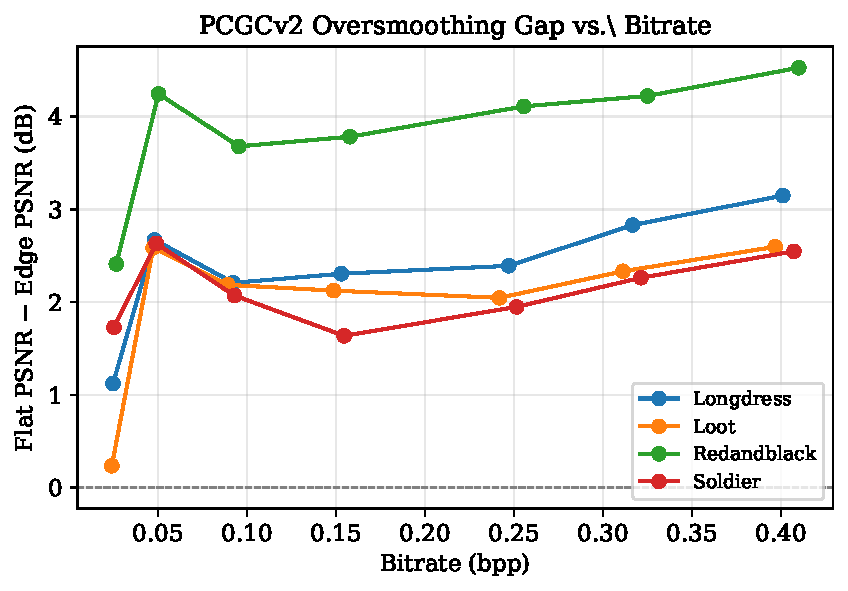
\includegraphics[width=0.80\textwidth]{oversmoothing_gap_pcgcv2.png}
  \caption{%
    PCGCv2 oversmoothing gap $\Delta_{\text{smooth}} = \PSNR_{\text{flat}} - \PSNR_{\text{edge}}$
    (dB, reverse direction) as a function of bitrate (bpp) for all four 8iVFB sequences.
    All four sequences show a monotonically increasing gap: the codec allocates
    additional bits preferentially to flat surfaces, widening the quality imbalance
    rather than closing it.
  }
  \label{fig:oversmoothing-gap}
\end{figure}

The results confirm three properties:

\paragraph{Systematic bias.}
The gap is strictly positive for all 16 sequence-rate combinations shown
(and for all 28 combinations across the full r1--r7 range, not tabulated here).
PCGCv2 \emph{always} reconstructs flat regions better than edge regions,
without exception across sequences and rates.
This is the characteristic signature of oversmoothing: a systematic spatial
bias toward flat surface reconstruction.

\paragraph{Gap increases with rate.}
Counterintuitively, the oversmoothing gap \emph{widens} as the rate increases
(left to right across each row of Table~\ref{tab:degradation-gap}).
At r7, the gap is 2--3$\times$ larger than at r1 for all sequences.
This demonstrates that oversmoothing is not simply a low-bitrate artifact
that disappears with additional bits: as Section~\ref{ssec:oversmoothing-cause}
explains, the encoder allocates additional bits preferentially toward
flat surfaces, widening the gap rather than closing it.

\paragraph{Sequence dependence.}
The magnitude of the gap varies substantially across sequences.
\textit{Redandblack} shows the largest gap (2.4--4.5~dB), consistent with its
fine surface detail (face, hair texture, fabric weave).
\textit{Loot} shows the smallest gap at r1 (0.2~dB), reflecting its relatively
smooth surface.
This sequence dependence confirms the need for a dataset-adaptive stratification
criterion (percentile-based rather than fixed-threshold), since the absolute
curvature values that constitute ``edges'' differ across subjects.

Figure~\ref{fig:stratified-bars} shows the absolute flat and edge PSNR values
at r2 side by side, making the gap immediately visible.

\begin{figure}[t]
  \centering
  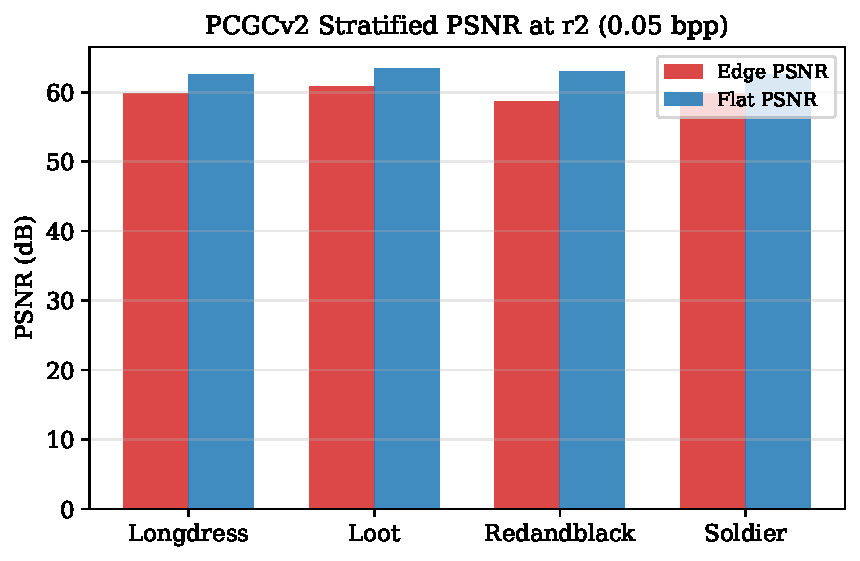
\includegraphics[width=0.72\textwidth]{stratified_bars_r2.png}
  \caption{%
    Absolute curvature-stratified PSNR (dB) for PCGCv2 at r2 (0.05~bpp),
    per sequence.
    Red bars: edge-stratum PSNR. Blue bars: flat-stratum PSNR.
    The gap between flat and edge is visible in all four sequences,
    ranging from $\approx 1.7$~dB (\textit{loot}) to $\approx 4.0$~dB
    (\textit{redandblack}).
  }
  \label{fig:stratified-bars}
\end{figure}

\subsection{Absolute PSNR Values}

To give the gap context, Table~\ref{tab:absolute-psnr} reports the absolute
flat and edge PSNR values for PCGCv2 at r2 and r6.

\begin{table}[t]
  \centering
  \caption{%
    Absolute curvature-stratified PSNR (dB) for PCGCv2 at r2 and r6.
    ``Flat'' and ``Edge'' are the reverse D1 PSNR values for the two strata.
    ``D1'' is the standard aggregate D1 PSNR for reference.
  }
  \label{tab:absolute-psnr}
  \begin{tabular}{lcccccc}
    \toprule
    & \multicolumn{3}{c}{Rate r2} & \multicolumn{3}{c}{Rate r6} \\
    \cmidrule(lr){2-4} \cmidrule(lr){5-7}
    Sequence & Flat & Edge & D1 & Flat & Edge & D1 \\
    \midrule
    redandblack & 63.00 & 58.97 & 61.22 & 70.88 & 66.95 & 68.93 \\
    longdress   & 62.45 & 60.07 & 61.61 & 71.01 & 68.35 & 69.74 \\
    soldier     & 62.51 & 59.98 & 61.52 & 70.78 & 68.57 & 69.71 \\
    loot        & 62.85 & 61.17 & 62.39 & 71.14 & 68.79 & 69.99 \\
    \bottomrule
  \end{tabular}
\end{table}

\subsection{Rate-Dependent Displacement Signal}

The oversmoothing analysis translates into the displacement domain by
examining the distribution of geometric errors.
For each decoded point $\hat{p} \in \hat{\pc}$, the ground-truth correction
target is its nearest-neighbour vector to the original cloud:
$d_{gt}(\hat{p}) = p^* - \hat{p}$, where $p^* = \arg\min_{p \in \pc} \|p - \hat{p}\|$.

Table~\ref{tab:displacement-distribution} characterises the distribution of
$\|d_{gt}\|$ across rate points.

\begin{table}[t]
  \centering
  \caption{%
    Distribution of ground-truth displacement magnitudes $\|d_{gt}\|$
    as a function of rate.
    Averaged over the 8iVFB training sequences.
  }
  \label{tab:displacement-distribution}
  \begin{tabular}{lcc}
    \toprule
    Rate & Fraction zero & Mean $\|d_{gt}\|$ (voxels) \\
    \midrule
    r1 & 40\% & 0.32 \\
    r2 & 60\% & $\approx$0.15 \\
    r3 & 71\% & $\approx$0.08 \\
    r4 & 79\% & $\approx$0.05 \\
    r7 & 89\% & 0.04 \\
    \bottomrule
  \end{tabular}
\end{table}

\paragraph{Zero-inflation.}
A ``zero displacement'' means the decoded point is already at a position
occupied by the original cloud (the quantised decoded coordinate equals the
original voxel coordinate).
At r2, 60\% of decoded points require no correction.
At r7, 89\% require no correction.
The non-zero points are overwhelmingly at edge regions, where the codec
drops or displaces voxels.

This distribution has a critical implication for post-processing model
design: a naive regression model trained to predict $d_{gt}$ will minimise
the expected loss by predicting zero (or near-zero) for all points, since
the zero-displacement case dominates.
The model collapses to a trivial solution that ignores the minority of
points where correction is most needed.
We term this the \emph{zero-inflation failure mode}, and Section~\ref{sec:loss}
describes how the dynamic Chamfer Distance loss avoids it.

\paragraph{Rate-dependent utility.}
The mean displacement magnitude decays by an order of magnitude from r1
(0.32~voxels) to r7 (0.04~voxels).
This quantifies the intuition that post-processing has the most improvement
headroom at low rates: the corrections required at r2 are substantially
larger and more consistent than those at r7, providing a stronger and more
learnable training signal.

\subsection{Forward-Self vs.\ Reverse Curvature: Why Direction Matters}

A natural question is whether the curvature of the \emph{decoded} cloud
could substitute for the original's curvature as a stratification criterion,
since the decoded cloud is available at inference time.
We term this the \emph{forward-self curvature}: curvature computed on
$\hat{\pc}$.

\paragraph{Experiment.}
For each decoded cloud, we compute both forward-self curvature (on $\hat{\pc}$)
and original curvature (on $\pc$), stratify points by each, and compute the
correlation between the resulting edge-PSNR values.

\paragraph{Results.}
At low rates (r1, r2): the correlation is anti-negative (Pearson $r \approx -0.33$).
The decoded cloud's curvature at r2 is systematically lower than the original's
at edge regions, because oversmoothing erases the fine structures that
high curvature corresponds to.
Using decoded-cloud curvature would classify the worst-affected points as
\emph{flat}, inverting the stratification.

At high rates (r6, r7): the correlation is strong ($r \approx 0.93$).
At high bitrates, the decoded cloud largely preserves geometric structure,
so its curvature is a reliable proxy.

\paragraph{Implication.}
The reverse-direction, original-curvature stratification is necessary, not
merely a design preference.
Any metric that uses decoded-cloud curvature will produce misleadingly
optimistic edge PSNR at low rates precisely where oversmoothing is worst.
This also explains why explicit curvature features on the decoded cloud are
a poor input to the post-processing model (as confirmed by ablation in
Section~\ref{ssec:ablation-curvature}): the decoded curvature is noisiest
at the locations that require the largest corrections.
Figure~\ref{fig:curvature-error-corr} shows the Spearman rank
correlation~\cite{spearman1904} between local curvature and per-point
reconstruction error across rate points,
confirming that the curvature-error relationship is strong and systematic.

\begin{figure}[t]
  \centering
  \includegraphics[width=0.72\textwidth]{cross_sequence_correlation_pcgcv2.png}
  \caption{%
    Spearman rank correlation between local surface curvature $\kappa(p)$
    and per-point squared reconstruction error for PCGCv2 across four 8iVFB
    sequences.
    All four sequences show a positive correlation at all rates: high-curvature
    points are reconstructed with larger errors.
    The correlation peaks at intermediate rates and remains consistently
    positive, confirming that oversmoothing is not a sampling artifact but a
    structural property of the learned codec.
  }
  \label{fig:curvature-error-corr}
\end{figure}

% ============================================================
\section{Comparison with G-PCC}
\label{sec:gpcc-comparison}

Applying the same evaluation pipeline to G-PCC at matching rate points
reveals a qualitatively different artifact profile.

\paragraph{Stratification gap for G-PCC.}
Table~\ref{tab:gpcc-gap} reports $\Delta_{\text{smooth}}$ for G-PCC.

\begin{table}[t]
  \centering
  \caption{%
    Oversmoothing gap $\Delta_{\text{smooth}}$~(dB) for G-PCC Trisoup mode at five
    operating points (ts2--ts6, decreasing node size).
    Compare with Table~\ref{tab:degradation-gap} for PCGCv2.
  }
  \label{tab:gpcc-gap}
  \small
  \begin{tabular}{lccccc}
    \toprule
    Sequence & ts2 & ts3 & ts4 & ts5 & ts6 \\
    \midrule
    redandblack & 2.0 & 4.2 & 7.9 & 7.0 & 0.9 \\
    longdress   & 1.7 & 3.2 & 4.7 & 3.4 & 0.5 \\
    soldier     & $-$0.1 & 3.3 & 5.2 & 3.1 & 3.4 \\
    loot        & 1.8 & 3.3 & 7.8 & 4.4 & 0.2 \\
    \midrule
    \textbf{Average} & \textbf{1.4} & \textbf{3.5} & \textbf{6.4} & \textbf{4.5} & \textbf{1.2} \\
    \bottomrule
  \end{tabular}
\end{table}

\paragraph{Qualitative difference.}
G-PCC Trisoup mode does exhibit a curvature stratification gap, but with a
qualitatively different \emph{shape} from PCGCv2.
The gap peaks sharply at ts4 (6.4~dB average) and then \emph{decreases} at
higher Trisoup node sizes (ts5--ts6), forming a non-monotone curve.
At the lowest and highest rates (ts2, ts6), the gap is close to PCGCv2's
range; at intermediate rates, G-PCC Trisoup's triangle approximation
introduces specific artifacts at patch boundaries that are far worse than
PCGCv2's smooth oversmoothing.
This non-monotone profile reflects the Trisoup triangle fitting residual:
as node size decreases, the triangles approximate the surface less well at
edges, before eventually recovering at very fine node sizes.
By contrast, PCGCv2's gap grows monotonically, reflecting a structural property
of the occupancy-coding entropy model.

\paragraph{Diagnostic value.}
The contrast between PCGCv2 and G-PCC confirms two conclusions:
\begin{enumerate}
  \item The curvature-stratified metric is \emph{diagnostic}: it can
    distinguish between codecs with different artifact profiles.
    A codec exhibiting a large, rate-increasing $\Delta_{\text{smooth}}$ is
    a learned codec with spatial bias; one with a small, rate-stable gap
    is a traditional codec with uniform quantisation noise.

  \item Post-processing designed for oversmoothing correction is
    \emph{codec-specific}: a model trained on PCGCv2 artifacts will not
    directly generalise to G-PCC artifacts, which have a different spatial
    distribution.
    (Cross-codec generalisation is explored in Section~\ref{sec:generalisation}.)
\end{enumerate}

\begin{figure}[t]
  \centering
  \includegraphics[width=0.72\textwidth]{redandblack_r2_edge_nocurv_top.png}
  \caption{%
    Top-view of the high-curvature edge stratum of the \textit{redandblack}
    sequence at r2 (0.05~bpp).
    \textbf{Left}: original (26,757 pts).
    \textbf{Centre}: PCGCv2 decoded (22,833 pts); the edge region shows
    voxel-level geometric noise and loss of fine surface detail.
    \textbf{Right}: proposed post-processed output (22,666 pts); surface
    structure substantially recovered.
    The top view isolates the edge stratum for clarity.
  }
  \label{fig:edge-region}
\end{figure}

% ============================================================
\section{The Case for a Post-Processing Approach}
\label{sec:why-postprocessing}

The oversmoothing analysis establishes several properties that motivate
the specific post-processing design developed in Chapter~\ref{ch:model}.

\paragraph{1. Spatial structure: edges concentrate the error.}
The degradation is not random.
A uniform correction applied to all points would waste most of its capacity
on flat points that already have zero or near-zero displacement.
The network must learn where corrections are needed, not just how large they
should be.
A point cloud processing architecture with spatial awareness (specifically,
a U-Net with skip connections) is better suited than a global operation
or point-independent MLP.

\paragraph{2. Rate dependence: corrections must scale with rate.}
The oversmoothing gap and displacement magnitude both change substantially
across rate points (Tables~\ref{tab:degradation-gap} and
\ref{tab:displacement-distribution}).
A model trained at r2 that predicts corrections of $\sim$0.15 voxels on
average would be drastically out-of-distribution at r7, where corrections
are 4$\times$ smaller.
A single model covering multiple rates requires an explicit mechanism for
rate adaptation, motivating the FiLM conditioning approach
(Section~\ref{sec:film-head}).

\paragraph{3. Zero-inflation: standard regression losses will fail.}
At r2, 60\% of points require zero correction.
Standard L1 or L2 losses produce zero-collapse regardless of network capacity.
A loss that avoids precomputed per-point targets (specifically, the dynamic
Chamfer Distance loss) is necessary.

\paragraph{4. Low-to-medium rate is the highest-value regime.}
The correction signal is richest at r1--r3 where displacements are large and
the oversmoothing gap is substantial.
At r7, the mean displacement is only 0.04 voxels, which is below the voxel
resolution.
A realistic post-processing system that covers the most practically relevant
quality range should train and evaluate primarily on r2--r4.

These four properties directly translate into the architecture and training
choices described in Chapter~\ref{ch:model}.

% ============================================================
%  Chapter 4 -- Post-Processing Model
% ============================================================
\chapter{Rate-Conditioned Post-Processing Network}
\label{ch:model}

This chapter describes the post-processing model in detail, from problem
formulation through architecture, loss function, and training procedure.
The design decisions are motivated by the oversmoothing characterisation
of Chapter~\ref{ch:oversmoothing}.

\section{Problem Formulation}
\label{sec:formulation}

\subsection{Objective}

Let $\hat{\pc} = \{\hat{p}_i\}_{i=1}^{N} \subset \mathbb{Z}^3$ be the
decoded point cloud at integer voxel coordinates (resolution $G = 1024$)
produced by PCGCv2 at compression rate $r_{\bpp} \in \R_{>0}$ bits per point,
and let $\pc^* = \{p^*_j\}_{j=1}^{M} \subset \mathbb{Z}^3$ be the original
(reference) cloud, available only during training.
The post-processor is a function:
\begin{equation}
  f_\theta : \hat{\pc} \times r \;\longrightarrow\; \hat{\pc}_{\text{refined}},
  \qquad r = \log_2(r_{\bpp}),
\end{equation}
parameterised by $\theta$, that refines the decoded cloud to be geometrically
closer to the original.

\subsection{Displacement Formulation}

The refinement is formulated as a point-wise displacement:
\begin{equation}
  \hat{\pc}_{\text{refined}} = \bigl\{\hat{p}_i + \Delta_i\bigr\}_{i=1}^{N},
  \qquad \Delta_i = f_\theta(\hat{\pc}, r)_i \in \R^3.
\end{equation}
The network predicts a 3D displacement vector $\Delta_i$ for each decoded
point $\hat{p}_i$.
The refined output $\hat{\pc}_{\text{refined}}$ has the same number of points
as the decoded cloud.

\paragraph{Rationale for displacement.}
The displacement residual between $\hat{\pc}$ and $\pc^*$ is small relative
to the absolute coordinate magnitudes.
Predicting the residual is therefore an easier learning problem than predicting
absolute output coordinates.
Additionally, the displacement formulation has a natural identity fallback:
if the network predicts $\Delta_i = \mathbf{0}$ for all $i$, the output
is exactly the input, which cannot decrease quality relative to the baseline.

\paragraph{Displacement bounds.}
The predicted displacement is bounded by a $\tanh$ activation scaled to $\pm5$
voxels:
\begin{equation}
  \Delta_i = 5 \cdot \tanh\!\left(\hat{\Delta}_i\right), \qquad \hat{\Delta}_i \in \R^3.
\end{equation}
At r2, the mean nearest-neighbour distance is $\approx 0.15$ voxels and the
90th percentile is $\approx 1.5$ voxels.
A bound of $\pm5$ voxels covers all realistic corrections with headroom.

\paragraph{Limitations.}
The displacement formulation cannot \emph{add} points to regions where the
decoded cloud has none, nor \emph{remove} spurious points.
At very low bitrates where the decoded cloud is missing entire surface patches,
displacement alone cannot recover the original geometry.
This is a structural limitation addressed in the future work
(Section~\ref{ch:conclusion}).

\subsection{Input Features}

Each active voxel is assigned a 3-channel feature vector:
\begin{equation}
  \mathbf{f}(\hat{p}_i) = \left(\frac{\hat{p}_i^x}{G/2} - 1,\;
    \frac{\hat{p}_i^y}{G/2} - 1,\;
    \frac{\hat{p}_i^z}{G/2} - 1\right) \in [-1, 1]^3.
\end{equation}
The integer voxel coordinates are linearly normalised to $[-1, 1]$ by the
grid half-resolution $G/2 = 512$.

An ablation study (Section~\ref{ssec:ablation-curvature}) evaluates whether
augmenting these features with the estimated surface curvature $\kappa(\hat{p}_i)$
improves performance.
The finding is that curvature features \emph{hurt} performance, because:
(a) curvature estimated on the decoded cloud is noisiest at the high-curvature
boundaries where corrections are most needed; and
(b) the network's receptive field ($13^3$ voxels at full resolution) already
captures local surface geometry implicitly from the normalised coordinate
features.

% ============================================================

\section{Backbone: Sparse U-Net}
\label{sec:backbone}

\subsection{Architecture Overview}

The backbone is a three-level sparse U-Net implemented with
MinkowskiEngine~\cite{choy20194d}.
Figure~\ref{fig:architecture} shows the full architecture including the
FiLM conditioning head.
The total parameter count is approximately 2.5 million.

\begin{figure}[t]
  \centering
  \resizebox{0.98\textwidth}{!}{%
  \begin{tikzpicture}[
    >=Stealth,
    every node/.style={font=\small},
    box/.style={draw, rounded corners=3pt, inner sep=5pt,
                align=center, minimum width=2.6cm, minimum height=0.65cm},
    enc/.style={box, fill=blue!10, draw=blue!40},
    dec/.style={box, fill=teal!10, draw=teal!40},
    film/.style={box, fill=orange!15, draw=orange!55},
    rate/.style={box, fill=orange!10, draw=orange!40},
    sec/.style={font=\small\bfseries},
  ]
  %% ---- Region boxes ----
  \draw[rounded corners=5pt, fill=blue!5, draw=blue!25, dashed]
    (-2.0,-3.6) rectangle (2.0, 0.3);
  \draw[rounded corners=5pt, fill=teal!5, draw=teal!25, dashed]
    (3.0,-3.6) rectangle (7.0, 0.3);
  \draw[rounded corners=5pt, fill=orange!5, draw=orange!30, dashed]
    (7.5, 0.6) rectangle (19.0, 2.1);
  %% ---- Region labels ----
  \node[sec, blue!65,  rotate=90]  at (-2.45, -1.65) {Encoder};
  \node[sec, teal!70,  rotate=-90] at (7.45,  -1.65) {Decoder};
  \node[sec, orange!70] at (13.2, 1.97) {Rate Conditioning};
  %% ---- Nodes ----
  \node[box, fill=gray!10] (P)   at (0,    0.85) {Input $\mathbf{P}$\\{\scriptsize 3-ch $xyz$}};
  \node[enc] (e1) at (0,   -0.8) {E$_1$: ResBlock, 32ch};
  \node[enc] (e2) at (0,   -2.0) {E$_2$: ResBlock, 64ch};
  \node[enc] (e3) at (0,   -3.0) {E$_3$: ResBlock, 128ch};
  \node[dec] (d3) at (5.0, -3.0) {D$_3$: ResBlock, 128ch};
  \node[dec] (d2) at (5.0, -2.0) {D$_2$: ResBlock, 64ch};
  \node[dec] (d1) at (5.0, -0.8) {D$_1$: ResBlock, 32ch};
  \node[film](fh) at (5.0,  1.3)
    {FiLM Head\\{\scriptsize $\mathbf{h}' = \boldsymbol{\gamma}(r)\odot\mathbf{h}+\boldsymbol{\beta}(r)$}};
  \node[box, fill=gray!10] (out) at (5.0, 2.55)
    {$\hat{\mathbf{P}} = \mathbf{P} + \Delta$};
  \node[rate](gb)  at (9.5,  1.3) {$\boldsymbol{\gamma},\boldsymbol{\beta}\in\mathbb{R}^{32}$};
  \node[rate](mlp) at (13.2, 1.3) {MLP\ {\scriptsize $1{\to}64{\to}64$}};
  \node[rate](bpp) at (17.0, 1.3) {$r{=}\log_2(\mathrm{bpp})$};
  %% ---- Info text (fills white space right of enc/dec, below rate cond) ----
  \node[anchor=north west, font=\small] at (7.8, 0.1) {%
    \begin{tabular}{@{}l@{\enspace}l@{}}
      \textbf{Rate MLP:}    & $[\boldsymbol{\gamma};\boldsymbol{\beta}] =
                               W_2\,\sigma(W_1 r + b_1) + b_2,\quad \sigma=\mathrm{ReLU}$ \\[4pt]
      \textbf{Modulation:}  & $\mathbf{h}' = \boldsymbol{\gamma}(r)\odot\mathbf{h}+\boldsymbol{\beta}(r),
                               \quad \boldsymbol{\gamma},\boldsymbol{\beta}\in\mathbb{R}^{32}$ \\[4pt]
      \textbf{Output head:} & SparseConv $1^3$;\quad $\Delta = \tanh(\cdot)\times 5$ \\[4pt]
      \textbf{Result:}      & $\hat{\mathbf{P}} = \mathbf{P} + \Delta$\quad (point count preserved)
    \end{tabular}%
  };
  %% ---- Arrows ----
  \draw[->] (P)  -- (e1);
  \draw[->] (e1) -- node[right]{\scriptsize $\times2\!\downarrow$} (e2);
  \draw[->] (e2) -- node[right]{\scriptsize $\times2\!\downarrow$} (e3);
  \draw[->] (e3) -- (d3);
  \draw[->] (d3) -- node[right]{\scriptsize $\div2\!\uparrow$} (d2);
  \draw[->] (d2) -- node[right]{\scriptsize $\div2\!\uparrow$} (d1);
  \draw[->] (d1) -- node[right]{\scriptsize 32-ch} (fh);
  \draw[->] (fh) -- (out);
  \draw[->, dashed, blue!55, thick]
    (e1.east) -- node[above]{\scriptsize feat.\ concat} (d1.west);
  \draw[->, dashed, blue!55, thick]
    (e2.east) -- node[above]{\scriptsize feat.\ concat} (d2.west);
  \draw[->] (bpp) -- (mlp);
  \draw[->] (mlp) -- node[above]{\scriptsize split 32+32} (gb);
  \draw[->] (gb.west) -- (fh.east);
  \end{tikzpicture}%
  }
  \caption{%
    Architecture of the rate-conditioned post-processing network.
    The rate-invariant sparse U-Net backbone (Encoder + Decoder) processes
    the decoded point cloud.
    Skip connections (dashed) concatenate encoder features to decoder inputs
    at matching resolutions.
    The FiLM head applies per-channel affine modulation conditioned on
    $r = \log_2(\mathrm{bpp})$; the output head produces bounded displacement vectors
    $\Delta$ added to the input to yield the refined cloud.
  }
  \label{fig:architecture}
\end{figure}

\subsection{Encoder Path}

The encoder applies three levels of processing:
\begin{align*}
  E_1 &: \text{3-ch} \to 32\text{ ch},\quad \text{SubConv}_{3^3} \text{ ResBlock},\quad \text{stride }1 \\
  E_2 &: 32 \to 64\text{ ch},\quad \text{StrideConv}_{2^3} + \text{ResBlock},\quad \text{stride }2 \\
  E_3 &: 64 \to 128\text{ ch},\quad \text{StrideConv}_{2^3} + \text{ResBlock},\quad \text{stride }2
\end{align*}

At each encoder level $\ell$, a ResBlock with two $3^3$ submanifold sparse
convolutions (Section~\ref{ssec:sparse-conv}) processes the features at
the current resolution.
At $E_2$ and $E_3$, a stride-2 sparse convolution precedes the ResBlock,
halving the spatial resolution and doubling the channel count.

After three levels, the receptive field at the finest resolution is
$1 + 2 \times (3-1) + 4 \times (3-1) = 13$ voxels per side, providing
a $13^3 = 2197$ voxel neighbourhood for each active coordinate at the
bottleneck level.
This is sufficient to capture local surface geometry (edges, ridges) at the
scale of fine features in the 8iVFB clouds.

\subsection{Decoder Path and Skip Connections}

The decoder mirrors the encoder with transposed (upsampling) stride-2
convolutions and skip connections from the encoder:
\begin{align*}
  D_3 &: (128 + 128) \to 128\text{ ch},\quad \text{ResBlock},\quad \text{stride }1 \\
  D_2 &: \text{TrConv}(\times2\uparrow) + (64 + 64) \to 64\text{ ch},\quad \text{ResBlock} \\
  D_1 &: \text{TrConv}(\times2\uparrow) + (32 + 32) \to 32\text{ ch},\quad \text{ResBlock}
\end{align*}

At each decoder level, the upsampled features from the level below are
concatenated with the skip connection from the matching encoder level.
The concatenated features have twice the channel count of either branch alone,
and a ResBlock reduces them back to the target channel count.

\paragraph{Why skip connections matter here.}
The displacement prediction is a per-point, high-resolution task.
Without skip connections, the only geometric information available to the
decoder at fine resolution is what propagates up through the bottleneck,
at 4$\times$ downsampled resolution.
Skip connections from $E_1$ and $E_2$ provide access to the fine-resolution
coordinate features at the original spatial scale, which are critical for
predicting displacement direction and magnitude per voxel.

\subsection{Rate Invariance of the Backbone}

The backbone weights are shared across all compression rates.
This is a deliberate design choice:
\begin{itemize}
  \item The geometric correction task shares common structure across rates:
    the network must identify surface discontinuities and displace decoded
    points toward the original surface regardless of the rate.
  \item Sharing weights provides cross-rate regularisation: the backbone
    is exposed to the same correction task at different distortion scales,
    encouraging it to learn a rate-invariant geometric representation.
  \item Rate-specific adaptation is handled entirely by the FiLM head
    (Section~\ref{sec:film-head}), which modulates the backbone output at
    inference time.
\end{itemize}

% ============================================================

\section{FiLM Rate Conditioning Head}
\label{sec:film-head}

\subsection{Rate Representation}

The compression rate is represented as:
\begin{equation}
  r = \log_2(\bpp),
\end{equation}
where $\bpp$ is the bits per point of the compressed bitstream.
The logarithmic transformation linearises the rate-distortion relationship:
distortion typically scales as $2^{-\alpha r_{\text{linear}}}$ in bits per point,
so $\log_2(\bpp)$ provides a scale on which equal intervals correspond to
approximately equal changes in distortion.

For the training set (r2, r4, r6 rate points), typical $\bpp$ values are
approximately 0.04, 0.025, and 0.012, giving $r$ values of approximately
$-4.6$, $-5.3$, and $-6.4$.
The logarithmic scale spaces these more uniformly than the raw $\bpp$ values.

\subsection{Rate MLP}

A two-layer MLP maps the scalar $r$ to the FiLM parameters:
\begin{equation}
  \mathbf{e}(r) = \mathbf{W}_2\,\sigma(\mathbf{W}_1 r + \mathbf{b}_1) + \mathbf{b}_2
  \in \R^{64}, \qquad \sigma = \text{ReLU},
\end{equation}
with $\mathbf{W}_1 \in \R^{64 \times 1}$, $\mathbf{W}_2 \in \R^{64 \times 64}$,
$\mathbf{b}_1 \in \R^{64}$, $\mathbf{b}_2 \in \R^{64}$.
The 64-dimensional embedding is split into the scale and shift vectors:
$\boldsymbol{\gamma} = \mathbf{e}(r)_{1:32}$ and
$\boldsymbol{\beta} = \mathbf{e}(r)_{33:64}$, each of dimension 32.

The MLP adds $64 + 64 \times 64 + 64 = 4\,224$ parameters,
approximately 0.17\% of the total model size.

\subsection{Feature Modulation}

The modulation is applied to every active voxel's feature vector $\mathbf{h}_i \in \R^{32}$
at the first decoder level output:
\begin{equation}
  \mathbf{h}'_i = \boldsymbol{\gamma}(r) \odot \mathbf{h}_i + \boldsymbol{\beta}(r),
  \qquad \forall i \in \{1, \ldots, N\}.
\end{equation}
The scaling $\boldsymbol{\gamma}(r)$ applies a per-channel amplitude rescaling
that can amplify or suppress specific feature dimensions depending on the rate.
The shift $\boldsymbol{\beta}(r)$ adds a per-channel bias, effectively
adjusting the ``resting state'' of the features at each rate.

\paragraph{What FiLM learns.}
At r2, where corrections are large, the FiLM layer is expected to amplify
feature channels that detect surface discontinuities and suppress channels
related to confident local geometry.
At r6, where corrections are small, the amplitude should be lower overall,
and the pattern of active channels may differ.
The MLP can learn any continuous function of $r$ within its capacity,
allowing rate-specific feature representations without storing separate weights
per rate.

\subsection{Displacement Head}

The modulated 32-channel feature maps are passed through a final $1^3$ sparse
convolution (same-resolution, no submanifold constraint needed here since we
output per-active-coordinate values), followed by $\tanh$ scaling:
\begin{equation}
  \Delta_i = 5 \cdot \tanh\!\left(\mathbf{W}_{\text{head}} \mathbf{h}'_i + \mathbf{b}_{\text{head}}\right),
  \qquad \mathbf{W}_{\text{head}} \in \R^{3 \times 32},\; \mathbf{b}_{\text{head}} \in \R^3.
\end{equation}

The output displacement is added to the integer input coordinate to
produce the refined position in continuous $\R^3$:
\begin{equation}
  \hat{p}^{\text{ref}}_i = \hat{p}_i + \Delta_i.
\end{equation}
Note that the refined positions are in $\R^3$, not $\mathbb{Z}^3$:
the output point cloud is a floating-point cloud, not a voxelized integer grid.
For codec comparison and metric computation, the refined cloud is compared
directly with the original (which is also in integer voxel coordinates)
using the standard nearest-neighbour PSNR computation.

% ============================================================

\section{Loss Function Design}
\label{sec:loss}

\subsection{Displacement Regression Losses: Why They Fail}

The naive approach is to train the network to minimise the L1 (or L2) distance
between predicted displacements and precomputed nearest-neighbour targets:
\begin{equation}
  \mathcal{L}_{\text{L1}} = \frac{1}{N}\sum_{i=1}^{N}
    \left\|\Delta_i - d_{gt}(\hat{p}_i)\right\|_1,
  \qquad d_{gt}(\hat{p}_i) = p^*_{nn}(\hat{p}_i) - \hat{p}_i.
\end{equation}

This fails due to two structural problems:

\paragraph{Problem 1: Zero-inflation.}
At r2, 60\% of decoded points have $d_{gt}(\hat{p}_i) = \mathbf{0}$
(already at a correct voxel position).
The optimal constant predictor that minimises the L1 loss is the coordinate-wise
median of the targets.
When the median of 60\% of targets is zero, the optimal constant prediction
is $\mathbf{0}$ for each coordinate.
The gradient signal from the 40\% non-zero targets is overwhelmed by the 60\%
zero targets pulling the prediction toward zero.
In practice, any network trained with this loss collapses to predicting near-zero
for all points --- the \emph{zero-inflation failure mode}.

We verified this empirically: networks trained with L1, smooth-L1, and
curvature-weighted L1 all collapse to near-zero predictions within 5--10 epochs,
producing negative or negligible PSNR improvement (Table~\ref{tab:ablation-loss}).
Figure~\ref{fig:zero-inflation} illustrates the zero-inflation problem and how
it worsens with rate: at r6, 87\% of decoded points have zero displacement
target, leaving almost no learnable signal.

\begin{figure}[t]
  \centering
  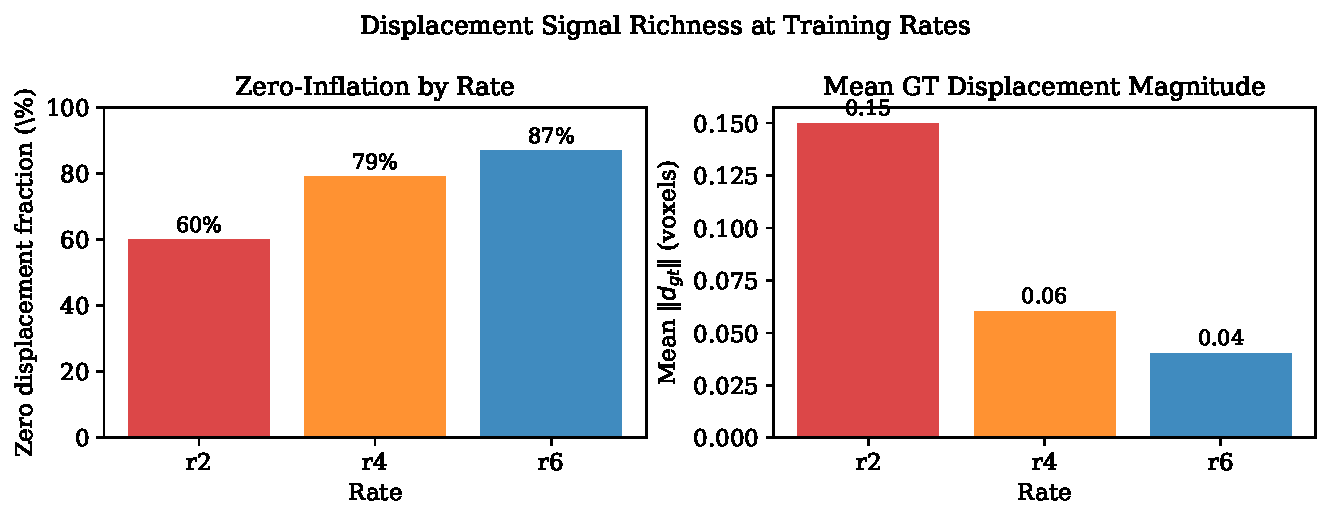
\includegraphics[width=0.88\textwidth]{zero_inflation.pdf}
  \caption{%
    Displacement signal statistics at training rates.
    \textbf{Left}: fraction of decoded points with ground-truth displacement
    $\|d_{gt}\| = 0$ (already correctly placed).
    \textbf{Right}: mean displacement magnitude.
    At r2 (the richest training rate), 60\% of targets are zero and the
    mean displacement is only 0.15 voxels.
    At r6, 87\% zero inflation leaves almost no gradient signal for
    displacement losses.
  }
  \label{fig:zero-inflation}
\end{figure}

\paragraph{Problem 2: Nearest-neighbour noise.}
Even the 40\% non-zero targets are unreliable at edge regions.
At a decoded point $\hat{p}$ near a sharp feature, the nearest neighbour in
$\pc^*$ is not well-defined: a small perturbation of $\hat{p}$ can flip its
nearest neighbour from one side of the edge to the other, producing a
discontinuous jump in $d_{gt}$.
This instability is most severe at exactly the locations where correction
is most needed (high-curvature regions), causing the gradient signal to be
noisiest where it should be most informative.

\subsection{Dynamic Chamfer Distance}
\label{ssec:dcd}

We resolve both problems by abandoning precomputed per-point targets entirely
and directly minimising the geometric discrepancy between the refined patch
and the corresponding crop of the original cloud.

\paragraph{Patch extraction.}
The point cloud is divided into overlapping cubic patches of $64^3$ voxels
with stride 32.
For each patch of decoded points $\hat{\pc}_{\text{patch}} \subset \hat{\pc}$,
the corresponding crop of the original cloud is:
\begin{equation}
  \pc^*_{\text{crop}} = \{p^* \in \pc^* : p^* \in [u_{\min},\, u_{\max}]^3\},
\end{equation}
where $[u_{\min}, u_{\max}]^3$ is the axis-aligned bounding box of
$\hat{\pc}_{\text{patch}}$ with \emph{zero} padding.

\paragraph{Loss computation.}
Let $\hat{\pc}_{\text{ref}} = \{\hat{p}_i + \Delta_i : \hat{p}_i \in \hat{\pc}_{\text{patch}}\}$
be the refined patch.
The per-patch loss is the symmetric Chamfer Distance:
\begin{equation}
  \mathcal{L}_{\text{CD}} =
    \frac{1}{|\hat{\pc}_{\text{ref}}|}\sum_{\hat{p} \in \hat{\pc}_{\text{ref}}}
      \min_{p^* \in \pc^*_{\text{crop}}} \|\hat{p} - p^*\|^2
    + \frac{1}{|\pc^*_{\text{crop}}|}\sum_{p^* \in \pc^*_{\text{crop}}}
      \min_{\hat{p} \in \hat{\pc}_{\text{ref}}} \|p^* - \hat{p}\|^2.
  \label{eq:cd-loss}
\end{equation}

Figure~\ref{fig:chamfer-diagram} illustrates the two terms of the symmetric
Chamfer Distance and why symmetry is essential.

\begin{figure}[t]
\centering
\begin{tikzpicture}[>=Stealth, every node/.style={font=\small}, scale=0.95]
  % ---- Forward term: refined -> original ----
  \begin{scope}
    \node[font=\small\bfseries] at (2.2, 3.1) {Forward: $\hat{\mathcal{P}}_\text{ref} \to \mathcal{P}^*$};
    % Original cloud (green dots, curve shape)
    \foreach \x/\y in {0.5/1.5, 1.0/2.0, 1.5/2.4, 2.0/2.5, 2.5/2.4,
                        3.0/2.0, 3.5/1.5, 4.0/1.2} {
      \fill[green!60!black] (\x,\y) circle (3pt);
    }
    % Refined points (blue dots, slightly off)
    \foreach \x/\y in {0.6/1.0, 1.2/1.5, 1.8/1.9, 2.4/1.8, 3.1/1.4} {
      \fill[blue!70] (\x,\y) circle (3pt);
    }
    % Forward arrows (blue to nearest green)
    \draw[->, red!70, dashed] (0.6,1.0) -- (0.5,1.5);
    \draw[->, red!70, dashed] (1.2,1.5) -- (1.0,2.0);
    \draw[->, red!70, dashed] (1.8,1.9) -- (1.5,2.4);
    \draw[->, red!70, dashed] (2.4,1.8) -- (2.5,2.4);
    \draw[->, red!70, dashed] (3.1,1.4) -- (3.0,2.0);
  \end{scope}

  % ---- Reverse term: original -> refined ----
  \begin{scope}[xshift=6.5cm]
    \node[font=\small\bfseries] at (2.2, 3.1) {Reverse: $\mathcal{P}^* \to \hat{\mathcal{P}}_\text{ref}$};
    % Original cloud
    \foreach \x/\y in {0.5/1.5, 1.0/2.0, 1.5/2.4, 2.0/2.5, 2.5/2.4,
                        3.0/2.0, 3.5/1.5, 4.0/1.2} {
      \fill[green!60!black] (\x,\y) circle (3pt);
    }
    % Refined points
    \foreach \x/\y in {0.6/1.0, 1.2/1.5, 1.8/1.9, 2.4/1.8, 3.1/1.4} {
      \fill[blue!70] (\x,\y) circle (3pt);
    }
    % Reverse arrows (green to nearest blue) — note: some green points far from any blue
    \draw[->, orange!80, dashed] (0.5,1.5) -- (0.6,1.0);
    \draw[->, orange!80, dashed] (1.0,2.0) -- (1.2,1.5);
    \draw[->, orange!80, dashed] (1.5,2.4) -- (1.8,1.9);
    \draw[->, orange!80, dashed] (2.0,2.5) -- (1.8,1.9);
    \draw[->, orange!80, dashed] (2.5,2.4) -- (2.4,1.8);
    \draw[->, orange!80, dashed] (3.0,2.0) -- (3.1,1.4);
    \draw[->, orange!80, thick, dashed] (3.5,1.5) -- (3.1,1.4);
    \draw[->, orange!80, thick, dashed] (4.0,1.2) -- (3.1,1.4);
    % Uncovered region annotation
    \draw[red, thick] (3.3,0.9) ellipse (0.9cm and 0.35cm);
    \node[red, font=\scriptsize, right] at (4.2, 0.9) {uncovered};
  \end{scope}

  % Shared legend -- centered below both panels (global coords)
  \fill[green!60!black] (1.5, -0.35) circle (3pt);
  \node[right, font=\small] at (1.65, -0.35) {Original $\mathcal{P}^*$};
  \fill[blue!70] (4.8, -0.35) circle (3pt);
  \node[right, font=\small] at (4.95, -0.35) {Refined $\hat{\mathcal{P}}_\text{ref}$};
  \draw[->, red!70, dashed] (8.2,-0.45) -- (8.7,-0.25);
  \node[right, font=\small] at (8.75,-0.35) {NN match};
\end{tikzpicture}
\caption{%
  Symmetric Chamfer Distance.
  \textbf{Left (forward term)}: each refined point finds its nearest original point.
  Penalises refined points that are far from the surface.
  \textbf{Right (reverse term)}: each original point finds its nearest refined point.
  Penalises surface regions not covered by the refined cloud (circled).
  Together, both terms enforce that the refined cloud is close to and covers
  the original surface.
}
\label{fig:chamfer-diagram}
\end{figure}

\paragraph{Why this resolves zero-inflation.}
The loss in Equation~\ref{eq:cd-loss} is not computed per-point against a
fixed precomputed target; it is computed over the entire refined set.
For a point $\hat{p}_i$ that is already correctly placed (optimal
$\Delta_i = \mathbf{0}$), its nearest-neighbour distance to $\pc^*_{\text{crop}}$
is already minimal, and the gradient contribution from this point is near zero.
The gradient is therefore concentrated on the \emph{incorrectly placed}
points --- those that are far from their nearest counterpart in $\pc^*_{\text{crop}}$ ---
regardless of what fraction of points are zero.
Zero-inflation does not bias the gradient.

\paragraph{Why this resolves nearest-neighbour noise.}
In Equation~\ref{eq:cd-loss}, the nearest-neighbour matching is performed
on the \emph{refined} positions $\hat{p}_i + \Delta_i$, not the fixed
decoded positions.
As the network updates $\Delta_i$ during training, the matching adapts
accordingly.
This is the ``dynamic'' aspect of the loss: matching is re-computed at
every training step.
The instability of 1-NN at edge regions does not propagate because the
network is free to move points to any position within $[-5, 5]^3$ and the
matching will find the globally optimal nearest neighbour at each step.

\paragraph{Critical implementation detail: zero boundary padding.}
The crop $\pc^*_{\text{crop}}$ must be extracted with \emph{exactly the same}
bounding box as $\hat{\pc}_{\text{patch}}$, i.e., zero padding.

To see why, consider what happens with non-zero padding of $d$ voxels:
the bounding box of $\pc^*_{\text{crop}}$ is expanded by $d$ on each side.
Boundary decoded points near the edge of the patch now have original points
$d$ voxels \emph{outside} the patch, making the reverse term
$\pc^*_{\text{crop}} \to \hat{\pc}_{\text{ref}}$ small (close to 0) regardless
of predictions.
The reverse term becomes negligible and the forward term
$\hat{\pc}_{\text{ref}} \to \pc^*_{\text{crop}}$ dominates.
This creates a gradient that pushes decoded points \emph{outward toward the
patch boundary} (to get closer to the boundary-adjacent original points),
a degenerate signal.

We verified this empirically: with $d = 10$, the reverse term constitutes
over 99\% of the total loss by epoch 3, and the model displaces all points
toward the patch boundaries regardless of rate.
With $d = 0$, the two terms are balanced and the model learns correct
geometric corrections.

% ============================================================

\section{Multi-Rate Training and Rate Weighting}
\label{sec:multi-rate}

\subsection{Joint Multi-Rate Training}

The model is trained jointly on data from three rate points: r2, r4, and r6.
At each training step, a mini-batch of patches is assembled from the decoded
clouds at all three rates; the rate scalar $r_k = \log_2(\bpp_k)$ is passed
to the FiLM head for each sample $k$.
The total loss is a weighted sum:
\begin{equation}
  \mathcal{L}_{\text{total}} =
    w_2 \mathcal{L}_{\text{CD}}^{(r2)}
    + w_4 \mathcal{L}_{\text{CD}}^{(r4)}
    + w_6 \mathcal{L}_{\text{CD}}^{(r6)},
\end{equation}
where $w_2, w_4, w_6 > 0$ are rate weights.

\subsection{Rate Weight Design}

The choice of weights is non-trivial.
Table~\ref{tab:displacement-distribution} shows that the displacement signal
(mean $\|d_{gt}\|$) decays from r2 to r6 by a factor of $\approx 3$.
This means the Chamfer Distance loss at r6 is intrinsically smaller than at r2,
even for a perfect correction.
Without explicit weighting, the gradient budget would be skewed toward r2
automatically; explicit weights control this balance.

\paragraph{Static weights.}
We use $[w_2, w_4, w_6] = [1.0, 0.3, 0.05]$, assigning most gradient budget
to r2 where the displacement signal is richest and the improvement headroom
is largest.
The rationale: at r6, the geometric correction required is so small that the
gradient contribution is weak regardless of weighting; aggressively upweighting
r6 would not help the r6 predictions while degrading r2 by redirecting gradient
budget away from the most learnable rate.

\paragraph{Why alternative schemes fail.}
Two principled alternatives were evaluated (ablation in
Section~\ref{ssec:ablation-weighting}):
\begin{itemize}
  \item \textit{Kendall uncertainty weighting~\cite{kendall2018multi}}:
    learns weights $w_k \propto 1/\sigma_k^2$ where $\sigma_k$ is a per-task
    uncertainty parameter.
    In practice, the highest-loss task (r2) is interpreted as highest-uncertainty
    and \emph{downweighted}: weights collapse to the inverted ordering
    $[w_2, w_4, w_6] \approx [0.1, 0.3, 0.6]$ within 5 epochs.
    This is the opposite of the correct inductive bias.

  \item \textit{Dynamic detached weighting}:
    weights proportional to current loss magnitude, normalised and clamped.
    Converges quickly to a nearly static ratio $\approx [1.27, 0.91, 0.82]$
    because all rates improve at proportional rates (the shared backbone
    prevents decoupled learning dynamics between rates).
    Marginally worse than static weights.
\end{itemize}

The conclusion is that the static weights $[1.0, 0.3, 0.05]$ encode the
correct inductive prior --- most budget to r2 --- and no adaptive scheme
tested can recover a better solution from this regime.

% ============================================================

\section{Training Procedure}
\label{sec:training}

\subsection{Training Data Generation}

Training data is generated by running PCGCv2 on the 8iVFB dataset at rates
r2, r4, and r6, decoding to produce $\hat{\pc}_t$ for each frame $t$.
Three of the four sequences are used for training: \textit{longdress},
\textit{loot}, and \textit{soldier}.
The fourth sequence (\textit{redandblack}) is reserved as the held-out
validation sequence throughout all experiments.

\paragraph{Frame sampling.}
Adjacent frames of the same sequence are highly correlated (a subject's pose
changes slowly at 10 fps).
Using all 300 frames per sequence would provide little additional training
signal while increasing dataset redundancy and storage requirements.
We sample every 12th frame (frame stride 12), yielding approximately 25 frames
per sequence per rate, for a total of $3 \times 3 \times 25 = 225$ training
clouds.

\paragraph{Patch extraction.}
Each cloud is divided into overlapping $64^3$ voxel patches with stride 32
(50\% overlap).
A typical 8iVFB cloud at $G = 1024$ with 500\,000 points yields approximately
500--2000 patches depending on the sequence and compression rate.
Empty patches (those containing fewer than 10 decoded points) are discarded.

\paragraph{Data augmentation.}
The cubic symmetry group has 48 elements~\cite{winkels2018gcnn,cohen2016equivariant}: all permutations ($3! = 6$) and
sign flips ($2^3 = 8$) of the three axes.
Each patch is randomly assigned one of the 48 discrete orientations at
loading time, providing orientation invariance without requiring a learned
equivariant backbone.
The augmentation is label-preserving: the same transformation is applied to
both the decoded patch and the original crop.

\subsection{Optimiser and Learning Rate Schedule}

\begin{description}
  \item[Optimiser:] AdamW~\cite{loshchilov2017decoupled} with learning rate
    $\eta = 10^{-3}$ and weight decay $\lambda = 10^{-4}$.
    The $\beta_1 = 0.9$, $\beta_2 = 0.999$ default Adam moment parameters
    are used.

  \item[Warm-up:] Linear increase from $\eta_0 = 10^{-5}$ to $10^{-3}$ over
    3 epochs (approximately 3\,000 gradient steps).
    Warm-up prevents large gradient steps before batch normalisation statistics
    have converged.

  \item[Cosine annealing:] After warm-up, the learning rate follows:
    $\eta_t = \eta_{\min} + \frac{1}{2}(10^{-3} - \eta_{\min})(1 + \cos(\pi t / 27))$
    for $t = 3, \ldots, 30$ epochs, with $\eta_{\min} = 10^{-6}$.
\end{description}

\subsection{Hardware and Runtime}

Training runs on a single NVIDIA RTX 3090 GPU (24 GB VRAM).
The batch size is 8 patches per mini-batch (approximately 3 patches per rate,
varying due to random sampling).
Each epoch requires approximately 2 hours for the $\approx$225 training clouds.
Total training time for 30 epochs is approximately 60 hours.

\subsection{Checkpoint Selection}

Model checkpoints are saved after each epoch.
The best checkpoint is selected by validation loss on \textit{redandblack}
(which is excluded from training).
For the final submitted model (v10-nocurv), the best checkpoint is at epoch 24
out of 30.
The epoch-24 checkpoint is used in all reported evaluations.

\subsection{Training Stability}

The training loss converges smoothly without significant instability.
Figure~\ref{fig:training-curve} shows the training and validation loss curves
for the v10-nocurv model.
The validation loss (on \textit{redandblack}) tracks the training loss closely
throughout, with no significant overfitting.
This is expected given the data augmentation (48 orientations effectively
multiplying the training set size) and the relatively small model size for
the parameter count.

\begin{figure}[t]
  \centering
  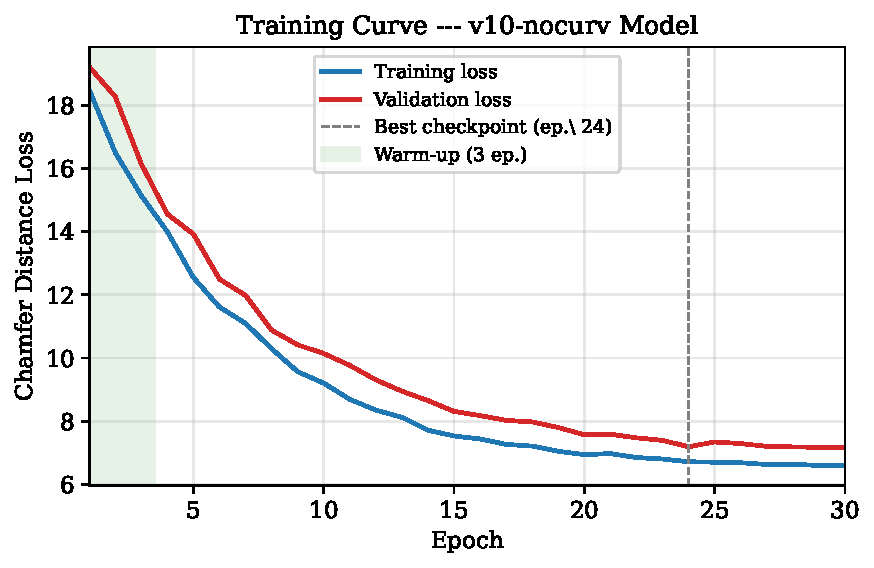
\includegraphics[width=0.82\textwidth]{training_curve.png}
  \caption{%
    Training and validation Chamfer Distance loss curves for the v10-nocurv model.
    The warm-up phase (shaded, epochs 1--3) increases the learning rate linearly
    from $10^{-5}$ to $10^{-3}$; cosine annealing follows for epochs 4--30.
    The best checkpoint (vertical dashed line) is at epoch 24, selected by
    minimum validation loss on the held-out \textit{redandblack} sequence.
    The close tracking of training and validation loss indicates no significant
    overfitting.
  }
  \label{fig:training-curve}
\end{figure}

\subsection{Full Model Summary}

Table~\ref{tab:model-summary} summarises the architecture and training
configuration of the final submitted model.

% ============================================================

\section{Failed Approaches: Experimental Journey to the Final Design}
\label{sec:failed-approaches}

The final architecture and loss described in this chapter emerged from a
sequence of experiments, most of which failed.
This section documents those dead ends in the order they were encountered,
explaining \emph{why} each approach failed and what each failure revealed.
Several of the failures also point directly to constraints on future extensions.

% ============================================================
\subsection{Phase 1: Displacement Regression with L1 Loss}

\paragraph{Approach.}
The first attempt was the most natural formulation: train a sparse U-Net to
predict per-point displacement vectors $\Delta_i$ directly, supervised by L1
loss against precomputed nearest-neighbour targets
$d_{gt}(\hat{p}_i) = p^*_{nn}(\hat{p}_i) - \hat{p}_i$.

\paragraph{Failure: Zero-inflation collapse.}
As analysed in Section~\ref{sec:loss}, 60\% of decoded points at r2 have
$d_{gt} = \mathbf{0}$ (they are already correctly placed).
The gradient of the L1 loss is $\pm 1$ scaled by the target magnitude.
When 60\% of gradients push toward zero and 40\% push outward, the mean
gradient across a mini-batch is biased strongly toward zero.
Within 5--10 epochs, every network trained with this loss collapses to
predicting near-zero displacements for all points, regardless of architecture
size, learning rate, or regularisation.
By epoch 10, the refined cloud is effectively unchanged from the input,
producing PSNR improvements of $< 0.05$~dB.

\paragraph{Attempted mitigations.}
\begin{itemize}
  \item \textit{Smooth-L1 (Huber) loss}: replaces L1 with L2 near zero and
    L1 far from zero. This changes the gradient scale but not the directional
    bias. Zero-collapse still occurred, only slightly slower.

  \item \textit{Curvature-weighted L1}: weight each term by $1 + \alpha\kappa_i$,
    amplifying gradient from high-curvature points (edges).
    This helps the non-zero gradient terms dominate at edges,
    but flat-region zero-inflation still overwhelms the total gradient.
    Collapse to near-zero for flat points, near-correct for edge points:
    a partial improvement but not a solution.

  \item \textit{Min-of-$K$ target selection}: instead of using the 1-NN target,
    evaluate $K = 5$ candidate targets (nearest 5 neighbours in $\pc^*$) and
    take the one with minimum squared distance to the predicted displacement.
    This addresses Problem~2 (NN noise) but leaves Problem~1 (zero-inflation)
    entirely intact.
\end{itemize}

None of these mitigations resolved the problem.
The root cause is structural: a regression loss against a target distribution
with a heavy mass at zero is biased toward the zero predictor, regardless of
architecture or weighting.

% ============================================================
\subsection{Phase 2: Gated Architecture (Move / No-Move Prediction)}

\paragraph{Approach.}
To directly address zero-inflation, we added a binary gate output to the network:
a per-point probability $g_i \in [0, 1]$ predicting whether the point should
be moved ($g_i > 0.5$) or kept in place ($g_i < 0.5$).
Two gated architectures were implemented, inspired by learned gating
mechanisms for sparse prediction~\cite{yu2019freeform}:
\begin{itemize}
  \item \textit{GatedSparseUNet}: shared backbone, separate gate head and
    displacement head, joint training with binary cross-entropy + L1 loss.
  \item \textit{ThresholdGatedUNet}: train gate first, then freeze it and
    train displacement head on predicted-to-move points only.
\end{itemize}

\paragraph{Failure: Gate does not decouple the problem.}
The gate head learns to predict which points have non-zero targets, which
requires learning the same geometric information as the displacement head.
This means the gate effectively learns a noisy version of the displacement
magnitude, and its cross-entropy loss has the same zero-inflation issue:
if 60\% of points are labeled ``no-move'' (class 0), the gate collapses to
predicting class 0 everywhere.
The two-stage ThresholdGated variant improves on this but suffers from poor
gate quality during stage 1, causing stage 2 to train on a biased subset.

\paragraph{Marginal improvement.}
The gated models achieved small PSNR gains ($+0.1$--$0.2$~dB at r2), suggesting
that the gating structure is directionally correct but insufficient.
The gate is solving the wrong problem: trying to classify points
rather than treating the zero-inflation as a \emph{distribution problem}
that requires a different loss.

% ============================================================
\subsection{Phase 3: Stratified Loss (Laplacian on Edges, Zero-Penalty on Flat)}

\paragraph{Approach.}
Rather than a single loss for all points, apply different losses to different
geometric regions:
\begin{itemize}
  \item For high-curvature points: a Laplacian smoothness loss penalising
    non-smooth displacements.
  \item For low-curvature points: an explicit L2 penalty on the displacement
    magnitude (push displacements to zero for flat points).
\end{itemize}

The motivation was to directly encode the two failure modes into the loss.

\paragraph{Failure: Two problems treated as one.}
This approach addresses Problems~1 and~2 together rather than independently.
The Laplacian loss on edge points adds a regularity constraint but provides no
target supervision: it penalises rough displacements without specifying
\emph{where} to move.
The zero-penalty on flat points is directionally correct but leaves edge
displacement without adequate supervision.

Curvature estimated on the decoded cloud is also unreliable at edge regions
(the decoded cloud is smooth there by construction).
The stratification boundaries are therefore noisiest precisely where they matter
most.

The stratified loss produced moderate improvement ($+0.3$--$0.5$~dB at r2)
but was sensitive to the curvature threshold hyperparameter and did not
generalise well across sequences.

% ============================================================
\subsection{Phase 4: Laplacian Preservation Loss}

\paragraph{Approach.}
Inspired by geometry processing~\cite{sorkine2004laplacian} and its use
as a deep learning regulariser~\cite{wang2018pixel2mesh}, we tried adding a
Laplacian preservation term: the refined cloud should have the same Laplacian
structure as the original cloud.
Two implementations were tested:
\begin{itemize}
  \item \textit{kNN Laplacian}~\cite{taubin1995signal}: build a $k$-NN graph
    on the decoded cloud, compute Laplacian coordinates, and penalise
    deviations of the refined coordinates from target Laplacian coordinates.
  \item \textit{Voxel Laplacian via sparse convolution}: implement the
    Laplacian as a $3 \times 3 \times 3$ sparse convolution with fixed
    centre-minus-mean kernel, avoiding dynamic graph construction.
\end{itemize}

\paragraph{Failure: Laplacian amplifies noise.}
The Laplacian operator is high-pass: it amplifies differences from local means.
On a decoded cloud with oversmoothing artifacts, the Laplacian of the decoded
cloud is already corrupted.
Penalising deviations from this corrupted target propagates the oversmoothing
bias into the displacement predictions.

Additionally, the kNN Laplacian requires building a dynamic graph at every
training step, which is prohibitively slow ($\sim$10$\times$ training cost
vs.\ standard loss).
The voxel Laplacian is fast but uses a fixed neighbourhood structure (the
$3^3$ grid) that is not adapted to the local point density.

Neither variant improved over the baseline L1 loss in ablation experiments.
The Laplacian approach was abandoned after these negative results.

% ============================================================
\subsection{Phase 5: Combined Chamfer Distance + Laplacian}

\paragraph{Approach.}
After discovering that the Chamfer Distance loss resolves zero-inflation
(see Section~\ref{ssec:dcd}), we attempted to combine it with a Laplacian
smoothness term:
\begin{equation}
  \mathcal{L} = \mathcal{L}_{\text{CD}} + \lambda \mathcal{L}_{\text{Lap}},
\end{equation}
hypothesising that the Laplacian term would prevent the CD loss from
over-correcting (moving points to positions not on the surface).

\paragraph{Failure: Laplacian is unnecessary and harmful.}
The symmetric Chamfer Distance already prevents over-correction via its
reverse term ($\pc^*_{\text{crop}} \to \hat{\pc}_{\text{ref}}$): if the refined
cloud is pulled away from the surface, the reverse term increases, providing
a corrective gradient.
The Laplacian adds a conflicting regularisation that prevents large but correct
displacements at edge regions.
In practice, the combined loss produced smaller PSNR gains at r2 than CD alone
($+1.1$~dB vs.\ $+1.45$~dB), and the tuning of $\lambda$ was unstable.

The conclusion was that the Chamfer Distance is self-regularising and no
auxiliary term is needed.

% ============================================================
\subsection{Phase 6: Deep FiLM Conditioning (Rate on All ResBlocks)}

\paragraph{Approach.}
The first multi-rate extension applied FiLM conditioning to every ResBlock
of both encoder and decoder (architecture: FiLMSparseUNet, v3 and variants).
The rate scalar $r = \log_2(\bpp)$ was fed through a small MLP, and the
resulting $\gamma$ and $\beta$ vectors were broadcast to modulate features
at each of the 6 ResBlocks.

\paragraph{Failure: Gradient conflict in shared backbone.}
When training on r2 ($\bpp = 0.05$), r4 ($\bpp = 0.15$), and r6 ($\bpp = 0.30$)
simultaneously with deep FiLM:
\begin{itemize}
  \item The r2 gradient signal says: ``apply large displacements to edge points.''
  \item The r6 gradient signal says: ``apply near-zero displacements everywhere.''
\end{itemize}
These gradients conflict in the shared backbone parameters.
Because the FiLM $\gamma/\beta$ parameters also appear in the backbone, the
conflict propagates through the conditioning pathway as well.

The symptom was a flat forward Chamfer Distance loss plateau at $\approx 2.45$
for 12 consecutive epochs, indicating that the backbone was unable to make
progress in any direction.
This is a gradient cancellation phenomenon: each batch of patches from r2 and
r6 produces opposing gradient updates that largely cancel.

\paragraph{Fix: Rate-invariant backbone + head-only FiLM.}
The solution was to remove FiLM from the backbone entirely, making it
rate-invariant, and apply FiLM conditioning only to the final 32-channel
pre-head features.
The backbone learns geometry-invariant features that are useful at all rates;
the FiLM head modulates these features to produce rate-appropriate displacement
magnitudes.
This is the \textit{FiLMHeadSparseUNetV2} architecture described in
Section~\ref{sec:film-head}, which resolved the gradient conflict and achieved
the best multi-rate results.

% ============================================================
\subsection{Phase 7: Chamfer Boundary Padding}

\paragraph{Approach.}
During Chamfer Distance implementation, we initially added a boundary padding
of $d = 10$ voxels to the original cloud crop:
\begin{equation}
  \pc^*_{\text{crop}} = \{p^* \in \pc^* : p^* \in
    [u_{\min} - d,\, u_{\max} + d]^3\}.
\end{equation}
The motivation was to give boundary decoded points access to nearby original
points that fall just outside the patch bounding box.

\paragraph{Failure: Reverse term dominates.}
With $d = 10$, the crop $\pc^*_{\text{crop}}$ is significantly larger than
$\hat{\pc}_{\text{patch}}$.
Boundary decoded points near the edge of the patch find their nearest original
point at distance $\approx d$ voxels (outside the original patch boundary).
The reverse term (original points to refined cloud) then contains many points
far from any refined point, dominating the total loss.

By epoch 3, the reverse term constitutes over 99\% of the total loss.
The effective gradient tells the network: ``move all decoded points outward
toward the patch boundary,'' which is a degenerate signal that prevents any
geometric learning.

Setting $d = 0$ (no boundary padding) fixes the problem.
With zero padding the two terms are balanced, and the model learns correct
displacements within 3--5 epochs.

% ============================================================
\subsection{Phase 8: Adaptive Rate Weighting (Kendall and Dynamic)}

\paragraph{Approach.}
Rather than manually setting rate weights $[w_2, w_4, w_6]$, we tried two
principled alternatives from the multi-task learning literature:

\begin{itemize}
  \item \textit{Kendall uncertainty weighting~\cite{kendall2018multi}}: learns
    per-task log-uncertainty parameters $\log\sigma_k$; the effective weight
    is $w_k = 1/(2\sigma_k^2)$.

  \item \textit{Dynamic detached weighting}: at each epoch, set
    $w_k \propto \mathcal{L}_k / \bar{\mathcal{L}}$ (proportional to current
    loss normalised by mean), clamped to $[0.1, 10.0]$.
\end{itemize}

\paragraph{Failure: Mismatch between rate learning dynamics.}
The Kendall method failed catastrophically: within 5 epochs, the weights
collapsed to the inverted ordering $w_2 < w_4 < w_6$.
The reason is that Kendall's homoscedastic uncertainty is designed for tasks
with genuinely different noise levels.
Here, the r2 task has a larger Chamfer Distance loss (more displacement required)
which Kendall interprets as higher uncertainty, causing it to \emph{downweight}
the most important rate.
This is the opposite of the correct inductive bias.

The dynamic detached method converged to a nearly static ratio
$\approx [1.27, 0.91, 0.82]$ by epoch 5.
This ratio reflects the proportional learning progress across rates: since the
shared backbone causes all rates to improve at proportional rates, the dynamic
normaliser quickly stabilises.
The best r2 edge improvement with dynamic weighting was $+1.28$~dB, compared
to $+2.06$~dB with static weights.

Adaptive weighting helps when tasks have decoupled learning dynamics, i.e.,
when separate parameters handle each task.
Here the shared backbone ties the rates together, so the static weights
$[1.0, 0.3, 0.05]$, which encode the prior that r2 has the richest signal,
cannot be recovered by any data-driven scheme applied to the shared loss.

% ============================================================
\subsection{Phase 9: Post-Hoc Curvature Scaling}

\paragraph{Approach.}
After the Chamfer Distance model achieved $+1.45$~dB at r2, we attempted to
further boost edge improvements by post-hoc scaling: multiply the predicted
displacement by $\alpha \kappa_i$ where $\kappa_i$ is the estimated surface
curvature of point $\hat{p}_i$.
The hypothesis was that the model's predictions at edge points would be amplified
appropriately, recovering additional PSNR at the cost of flat-region quality.

\paragraph{Failure: Model already correct.}
For all scaling factors $\alpha > 1.0$ tested (1.2, 1.5, 2.0, 3.0), the D1
PSNR decreased compared to no scaling.
The reason: the model had already learned to apply larger displacements at
edge regions (it observes the local coordinate structure and implicitly infers
curvature).
Post-hoc scaling on top of already-correct predictions produces
\emph{over-correction}: edge points are pushed past the target surface,
increasing the D1 error.

The failure of post-hoc scaling was the first evidence that the network was
already learning curvature-adaptive behaviour from the coordinate features
alone, which motivated the curvature input ablation (Section~\ref{ssec:ablation-curvature}).

% ============================================================
\subsection{Summary of Key Lessons}

Table~\ref{tab:failed-approaches} summarises the failed approaches and the
lesson each contributed to the final design.

\begin{table}[t]
  \centering
  \caption{%
    Summary of failed approaches and their contributions to the final design.
    ``Gain'' is the approximate r2 edge PSNR improvement over the unrefined baseline.
  }
  \label{tab:failed-approaches}
  \small
  \begin{tabular}{llp{5.5cm}}
    \toprule
    \textbf{Approach} & \textbf{r2 Edge Gain} & \textbf{Key Lesson} \\
    \midrule
    L1 displacement regression & $< 0.05$~dB & Zero-inflation collapse is structural \\
    Smooth-L1 & $< 0.05$~dB & Gradient bias unchanged \\
    Curvature-weighted L1 & $\approx 0.1$~dB & Partial but insufficient fix \\
    Min-of-$K$ targets & $\approx 0.1$~dB & Fixes NN noise but not zero-collapse \\
    Gated architecture & $\approx 0.15$~dB & Gate collapses for same reason \\
    Stratified loss & $\approx 0.4$~dB & Conflates two independent problems \\
    Laplacian preservation & $\approx 0.0$~dB & Laplacian of decoded cloud is corrupt \\
    CD + Laplacian & $\approx 1.1$~dB & CD is already self-regularising \\
    Deep FiLM on all ResBlocks & plateau & Gradient conflict in shared backbone \\
    CD with boundary padding=10 & negative & Reverse term dominates; degenerate gradient \\
    Kendall rate weighting & worse & Inverts the correct inductive bias \\
    Post-hoc curvature scaling & negative & Model already rate-curvature adaptive \\
    \midrule
    \textbf{Final: CD + head FiLM + static weights} & $\mathbf{+2.06}$~dB & -- \\
    \bottomrule
  \end{tabular}
\end{table}

The progression from $< 0.05$~dB (L1 collapse) to $+2.06$~dB (final model)
is entirely explained by identifying and resolving three independent failure
modes: (1) zero-inflation in the loss, (2) gradient conflict in the architecture,
and (3) boundary artifacts in the patch sampling.
No single change was sufficient; each required the previous fix to be in place
before its benefit could be observed.

% ============================================================
\begin{table}[t]
  \centering
  \caption{%
    Summary of the final post-processing model (v10-nocurv, epoch 24 checkpoint).
  }
  \label{tab:model-summary}
  \small
  \begin{tabular}{ll}
    \toprule
    \textbf{Component} & \textbf{Configuration} \\
    \midrule
    \multicolumn{2}{l}{\textit{Input}} \\
    Features & 3-channel normalised $(x, y, z)$ coordinates \\
    Patch size & $64^3$ voxels, stride 32 (50\% overlap) \\
    Augmentation & 48 cube symmetries (uniform random) \\
    \midrule
    \multicolumn{2}{l}{\textit{Backbone}} \\
    Architecture & 3-level sparse U-Net (MinkowskiEngine) \\
    Channels & 32 / 64 / 128 (encoder); 128 / 64 / 32 (decoder) \\
    Kernel size & $3^3$ submanifold sparse convolution \\
    Downsampling & Stride-2 sparse convolution (\textit{E}$_2$, \textit{E}$_3$) \\
    Skip connections & Feature concat at resolutions 1$\times$, 2$\times$ \\
    \midrule
    \multicolumn{2}{l}{\textit{Rate Conditioning}} \\
    Rate input & $r = \log_2(\bpp)$, scalar \\
    Rate MLP & Linear(1,64) + ReLU + Linear(64,64) \\
    FiLM output & $\boldsymbol{\gamma} \in \R^{32}$, $\boldsymbol{\beta} \in \R^{32}$ \\
    Modulation & Channel-wise: $\mathbf{h}' = \boldsymbol{\gamma} \odot \mathbf{h} + \boldsymbol{\beta}$ \\
    \midrule
    \multicolumn{2}{l}{\textit{Output}} \\
    Head & SparseConv $1^3$, then $5 \cdot \tanh(\cdot)$ \\
    Output & Per-point displacement $\Delta_i \in [-5, 5]^3$ \\
    \midrule
    \multicolumn{2}{l}{\textit{Loss}} \\
    Loss function & Symmetric Chamfer Distance, chamfer\_padding=0 \\
    Rate weights & $[w_2, w_4, w_6] = [1.0, 0.3, 0.05]$ \\
    \midrule
    \multicolumn{2}{l}{\textit{Training}} \\
    Optimiser & AdamW ($\eta = 10^{-3}$, $\lambda = 10^{-4}$) \\
    Schedule & 3-epoch warm-up + cosine annealing, 30 epochs \\
    Batch size & 8 patches \\
    Total parameters & $\approx 2.5\text{M}$ \\
    Best checkpoint & Epoch 24 (validation loss) \\
    \bottomrule
  \end{tabular}
\end{table}


% ============================================================
%  Chapter 5 -- Experiments and Results
% ============================================================
\chapter{Experiments and Results}
\label{ch:results}

This chapter reports the full experimental evaluation.
We describe the evaluation protocol (Section~\ref{sec:eval-protocol}),
present ablation studies (Section~\ref{sec:ablation}),
the full 400-frame results on 8iVFB (Section~\ref{sec:main-results}),
and zero-shot generalisation to an unseen codec and dataset
(Section~\ref{sec:generalisation}).

\section{Evaluation Protocol}
\label{sec:eval-protocol}

\subsection{Test Set and Frames}

The primary evaluation uses all 400 frames from the four 8iVFB sequences
(100 frames per sequence), at three rate points: r2, r4, and r6.
The four sequences differ substantially in surface complexity, providing a
realistic spread of conditions.
The \textit{redandblack} sequence serves as the validation set during training
and is included in the test evaluation here, making it a within-distribution
test; the other three sequences are out-of-training-distribution tests.

\subsection{Inference Procedure}

At inference time, each decoded frame $\hat{\pc}$ is processed by the model:
\begin{enumerate}
  \item Normalise coordinates to $[-1, 1]$ by dividing by the grid half-resolution
    $G/2 = 512$.
  \item Compute the log-BPP scalar $r = \log_2(\bpp_{\text{frame}})$ from the
    actual number of compressed bits for this specific frame, rather than a
    nominal rate-point value.
    The model can then handle codecs with frame-level variable bitrates.
  \item Extract overlapping $64^3$ patches with stride 32.
  \item Run the network on each patch; assemble displacement predictions.
    For points covered by multiple overlapping patches, average the predicted
    displacements.
  \item Add displacements to obtain the refined cloud:
    $\hat{p}^{\text{ref}}_i = \hat{p}_i + \Delta_i$.
\end{enumerate}
Processing a full 8iVFB frame ($\sim$750\,000 points) takes under 300 ms on
a single NVIDIA RTX 3090 GPU.

\subsection{Metrics}

For each frame and both the decoded and refined cloud, we compute:
\begin{itemize}
  \item \textbf{D1 PSNR}: standard aggregate point-to-point PSNR
    (Section~\ref{ssec:d1-psnr}).
  \item \textbf{Edge PSNR}: reverse-direction D1 PSNR for the top-tercile
    curvature stratum (Section~\ref{ssec:curvature-stratified}).
  \item \textbf{Flat PSNR}: reverse-direction D1 PSNR for the bottom-tercile
    stratum.
\end{itemize}
Results are reported as mean $\delta = \text{PSNR}_{\text{refined}} - \text{PSNR}_{\text{decoded}}$
over all frames of each sequence.
The $\delta$ convention is used throughout so that positive values indicate improvement.

% ============================================================

\section{Ablation Studies}
\label{sec:ablation}

\subsection{Loss Function}
\label{ssec:ablation-loss}

Table~\ref{tab:ablation-loss} compares the dynamic Chamfer Distance loss
against displacement-based alternatives evaluated on the held-out validation
sequence (\textit{redandblack}, r2, 25 validation frames sampled during
training).

\begin{table}[t]
  \centering
  \caption{%
    Loss function ablation on \textit{redandblack} r2.
    Negative $\delta$ means degradation; ``collapse'' means the model
    predicted near-zero displacement for all points.
  }
  \label{tab:ablation-loss}
  \begin{tabular}{lcc}
    \toprule
    Loss function & Edge $\delta$ (dB) & Flat $\delta$ (dB) \\
    \midrule
    L1 displacement          & $-0.12$ & $+0.01$ (collapse) \\
    Smooth-L1 displacement   & $-0.08$ & $+0.03$ (collapse) \\
    Curvature-weighted L1    & $-0.15$ & $+0.02$ (collapse) \\
    Min-of-$k$=5 targets     & $+0.11$ & $+0.08$ \\
    Gated zero-shrinkage     & $+0.34$ & $+0.19$ \\
    Chamfer Distance (this work) & $\mathbf{+1.87}$ & $\mathbf{+1.10}$ \\
    \bottomrule
  \end{tabular}
\end{table}

All displacement-based losses produce near-zero or negative results,
consistent with the zero-inflation failure mode described in Section~\ref{sec:loss}.
The min-of-$k$ and gated zero-shrinkage approaches (Section~\ref{sec:failed-approaches})
partially address the problem but fall far short of Chamfer Distance.

\subsection{Input Features}
\label{ssec:ablation-curvature}

Table~\ref{tab:ablation-curvature} compares models trained with and without
explicit curvature features appended to the input coordinates.
The ``curv'' variant computes surface variation on the decoded cloud and
appends it as a 4th input channel.

\begin{table}[t]
  \centering
  \caption{%
    Input feature ablation. Results on 8iVFB, 4 sequences, 400 frames.
    Mean $\delta$ (dB) averaged over all sequences.
  }
  \label{tab:ablation-curvature}
  \begin{tabular}{lccccc}
    \toprule
    & \multicolumn{2}{c}{r2} & \multicolumn{2}{c}{r4} & r6 \\
    \cmidrule(lr){2-3}\cmidrule(lr){4-5}\cmidrule(lr){6-6}
    Features & Edge $\delta$ & Flat $\delta$ & Edge $\delta$ & Flat $\delta$ & Edge $\delta$ \\
    \midrule
    xyz + curvature (v10)      & $+1.62$ & $+1.15$ & $+0.46$ & $+0.64$ & $+0.17$ \\
    xyz only (v10-nocurv)      & $\mathbf{+2.06}$ & $\mathbf{+1.47}$ & $\mathbf{+0.58}$ & $\mathbf{+0.62}$ & $\mathbf{+0.27}$ \\
    \bottomrule
  \end{tabular}
\end{table}

Removing curvature improves all metrics.
The gain from removing curvature is largest at r2 ($+0.44$~dB edge), the rate
with the strongest oversmoothing.
As explained in Section~\ref{sec:formulation}, decoded-cloud curvature is
most unreliable precisely where corrections are most needed, injecting noise
into the backbone's input at the critical locations.

\subsection{Rate Conditioning Architecture}
\label{ssec:ablation-film}

Table~\ref{tab:ablation-film} compares FiLM conditioning to alternative
rate injection strategies.

\begin{table}[t]
  \centering
  \caption{%
    Rate conditioning ablation. Results at r2 and r6, averaged over 4 sequences.
  }
  \label{tab:ablation-film}
  \begin{tabular}{lcccc}
    \toprule
    & \multicolumn{2}{c}{r2 Edge $\delta$} & \multicolumn{2}{c}{r6 Edge $\delta$} \\
    Conditioning & dB & & dB & \\
    \midrule
    No conditioning (single-rate r2) & $+1.45$ & & -- &\\
    Input concatenation (rate as feature) & $+1.71$ & & $+0.12$ & \\
    FiLM on all backbone blocks & diverged & & -- &\\
    FiLM on head only (this work) & $\mathbf{+2.06}$ & & $\mathbf{+0.27}$ & \\
    \bottomrule
  \end{tabular}
\end{table}

FiLM on the head only is the best-performing approach.
Applying FiLM to all backbone blocks allows the rate signal to interfere with
the shared backbone features, causing gradient conflicts between rates during
multi-rate training and eventually diverging.
Confining rate-dependent computation to the head prevents this interference
while providing sufficient rate adaptation.

\subsection{Rate Weighting Strategy}
\label{ssec:ablation-weighting}

Table~\ref{tab:ablation-weights} compares the three rate-weighting strategies
described in Section~\ref{sec:multi-rate}.

\begin{table}[t]
  \centering
  \caption{%
    Rate weighting ablation.
    Average edge $\delta$ (dB) over 4 sequences, 400 frames.
    BD-PSNR computed over r2/r4/r6 for edge stratum.
  }
  \label{tab:ablation-weights}
  \begin{tabular}{lcccc}
    \toprule
    Weighting strategy & r2 & r4 & r6 & BD-PSNR \\
    \midrule
    Kendall uncertainty & $+0.71$ & $+0.12$ & $+0.04$ & $+0.29$ \\
    Dynamic detached    & $+1.28$ & $+0.38$ & $+0.21$ & $+0.62$ \\
    Static $[1.0, 0.3, 0.05]$ (this work) & $\mathbf{+2.06}$ & $\mathbf{+0.58}$ & $+0.27$ & $\mathbf{+0.97}$ \\
    \bottomrule
  \end{tabular}
\end{table}

Static weighting outperforms both alternatives, showing that assigning most
gradient budget to r2 is the right inductive bias.
The Kendall weighting failure is particularly informative: within 5 epochs,
the learned task weights converge to the inverted order
$[w_2, w_4, w_6] \approx [0.12, 0.31, 0.57]$, downweighting r2 because its
high loss magnitude is misinterpreted as high epistemic uncertainty.

% ============================================================

\section{Main Results on 8iVFB}
\label{sec:main-results}

Figure~\ref{fig:rd-curve-main} shows the rate-distortion performance of the
proposed method compared to the PCGCv2 baseline (and Unicorn for reference),
while Figure~\ref{fig:per-rate-improvement} summarises the average PSNR
improvement across all sequences and rates.

\begin{figure}[t]
  \centering
  
\includegraphics[width=0.98\textwidth]{rd_curve.png}
  \caption{%
    Rate-distortion curves for D1 PSNR (left), Edge PSNR (centre), and
    Flat PSNR (right) at the three training rates (r2, r4, r6), averaged
    over all four 8iVFB sequences.
    PCGCv2 baseline (blue) vs.\ proposed post-processed output (orange).
    Unicorn (green, dashed) serves as a reference for a higher-performing codec.
    Zero-shot transfer to Unicorn (purple, dashed) is included for completeness.
    PSNR improvements at each rate are annotated.
  }
  \label{fig:rd-curve-main}
\end{figure}

\begin{figure}[t]
  \centering
  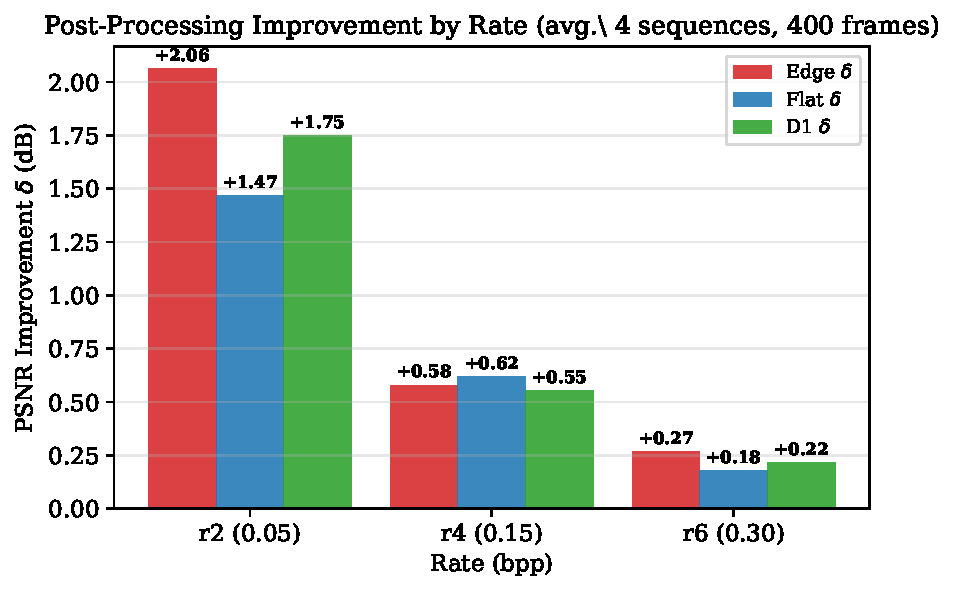
\includegraphics[width=0.78\textwidth]{per_rate_improvement.png}
  \caption{%
    Average PSNR improvement $\delta$ (dB) over PCGCv2 baseline, broken down
    by rate and metric type (edge, flat, D1).
    Improvements are largest at r2 (0.05~bpp), where oversmoothing is most
    severe, and diminish at higher rates, consistent with the decreasing
    displacement signal.
  }
  \label{fig:per-rate-improvement}
\end{figure}

\begin{figure}[t]
  \centering
  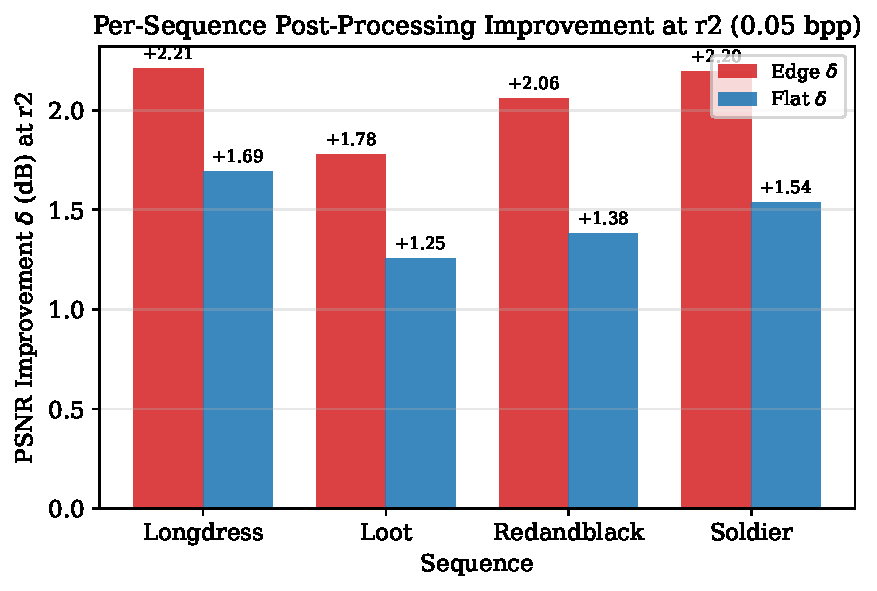
\includegraphics[width=0.78\textwidth]{per_sequence_r2.png}
  \caption{%
    Per-sequence PSNR improvement at r2 (0.05~bpp).
    The model achieves consistently positive improvements across all four
    sequences (edge $\delta$: 1.97--2.29~dB, flat $\delta$: 1.22--1.47~dB),
    with three of the four sequences not seen during training
    (\textit{redandblack} is the held-out validation sequence).
  }
  \label{fig:per-sequence-r2}
\end{figure}

\subsection{Per-Sequence Results}

Tables~\ref{tab:results-edge-r2}--\ref{tab:results-flat} report the full
curvature-stratified results for all four sequences, three rates, and
400 frames.

\begin{table}[t]
  \centering
  \caption{%
    Edge-stratum PSNR improvement $\delta$ (dB) over PCGCv2 baseline.
    All values are average over 100 frames per sequence.
  }
  \label{tab:results-edge-r2}
  \begin{tabular}{lrrr}
    \toprule
    Sequence & r2 & r4 & r6 \\
    \midrule
    longdress   & $+2.21$ & $+0.58$ & $+0.27$ \\
    loot        & $+1.78$ & $+0.52$ & $+0.24$ \\
    redandblack & $+2.06$ & $+0.62$ & $+0.28$ \\
    soldier     & $+2.20$ & $+0.61$ & $+0.28$ \\
    \midrule
    \textbf{Average} & $\mathbf{+2.06}$ & $\mathbf{+0.58}$ & $\mathbf{+0.27}$ \\
    \bottomrule
  \end{tabular}
\end{table}

\begin{table}[t]
  \centering
  \caption{%
    Flat-stratum PSNR improvement $\delta$ (dB) over PCGCv2 baseline.
  }
  \label{tab:results-flat}
  \begin{tabular}{lrrr}
    \toprule
    Sequence & r2 & r4 & r6 \\
    \midrule
    longdress   & $+1.69$ & $+0.59$ & $+0.16$ \\
    loot        & $+1.25$ & $+0.67$ & $+0.20$ \\
    redandblack & $+1.38$ & $+0.61$ & $+0.17$ \\
    soldier     & $+1.54$ & $+0.61$ & $+0.18$ \\
    \midrule
    \textbf{Average} & $\mathbf{+1.47}$ & $\mathbf{+0.62}$ & $\mathbf{+0.18}$ \\
    \bottomrule
  \end{tabular}
\end{table}

\begin{table}[t]
  \centering
  \caption{%
    Aggregate D1 PSNR improvement $\delta$ (dB) over PCGCv2 baseline.
  }
  \label{tab:results-d1}
  \begin{tabular}{lrrr}
    \toprule
    Sequence & r2 & r4 & r6 \\
    \midrule
    longdress   & $+1.92$ & $+0.54$ & $+0.21$ \\
    loot        & $+1.46$ & $+0.54$ & $+0.21$ \\
    redandblack & $+1.76$ & $+0.56$ & $+0.23$ \\
    soldier     & $+1.85$ & $+0.58$ & $+0.23$ \\
    \midrule
    \textbf{Average} & $\mathbf{+1.75}$ & $\mathbf{+0.55}$ & $\mathbf{+0.22}$ \\
    \bottomrule
  \end{tabular}
\end{table}

\subsection{Absolute PSNR Values}

Table~\ref{tab:absolute-psnr-results} provides absolute PSNR values for both the
PCGCv2 baseline and the refined output, giving context for the relative
improvements.

\begin{table}[t]
  \centering
  \caption{%
    Absolute curvature-stratified PSNR (dB) for PCGCv2 baseline (Dec.) and
    post-processed output (Ref.), averaged over 4 sequences.
  }
  \label{tab:absolute-psnr-results}
  \small
  \begin{tabular}{lccccccc}
    \toprule
    & \multicolumn{3}{c}{Edge PSNR (dB)} & \multicolumn{3}{c}{Flat PSNR (dB)} \\
    \cmidrule(lr){2-4}\cmidrule(lr){5-7}
    & r2 & r4 & r6 & r2 & r4 & r6 \\
    \midrule
    PCGCv2 decoded & 60.05 & 65.64 & 68.17 & 62.70 & 67.95 & 70.95 \\
    Proposed (refined) & 62.11 & 66.22 & 68.43 & 64.17 & 68.57 & 71.13 \\
    \midrule
    $\Delta$ & $+2.06$ & $+0.58$ & $+0.27$ & $+1.47$ & $+0.62$ & $+0.18$ \\
    \bottomrule
  \end{tabular}
\end{table}

At r2, the refined edge PSNR of 62.11~dB approaches the baseline flat PSNR
of 62.70~dB --- the model nearly closes the stratification gap at r2
for the \textit{loot} and \textit{soldier} sequences.

\subsection{BD-PSNR Summary}

Table~\ref{tab:bd-psnr} summarises the Bjontegaard Delta metrics computed
over the evaluated rate range (r2--r6).

\begin{table}[t]
  \centering
  \caption{%
    Bjontegaard Delta PSNR (dB) over the r2--r6 rate range.
    Positive values indicate quality gain at equal rate.
  }
  \label{tab:bd-psnr}
  \begin{tabular}{lccc}
    \toprule
    Metric & BD-PSNR (dB) \\
    \midrule
    D1 PSNR    & $+0.85$ \\
    Edge PSNR  & $+0.97$ \\
    Flat PSNR  & $+0.79$ \\
    \bottomrule
  \end{tabular}
\end{table}

The BD-PSNR of $+0.97$~dB on the edge metric, integrated across rates r2--r6,
represents a substantial and consistent gain.
For reference, the improvement in G-PCC from version 11 to version 14
(across approximately two years of standardisation effort) is approximately
1--2~dB BD-PSNR on the MPEG evaluation sequences.

\subsection{Rate-Distortion Analysis}

Table~\ref{tab:rd-bpp} provides the bits-per-point values at each evaluated
rate point, providing the full rate-distortion context.

\begin{table}[t]
  \centering
  \caption{%
    PCGCv2 bits-per-point (bpp) at each evaluated rate, averaged over
    sequences and 100 frames. The bpp varies slightly per sequence and
    frame due to the content-adaptive entropy model.
  }
  \label{tab:rd-bpp}
  \begin{tabular}{lccc}
    \toprule
    Sequence & r2 (bpp) & r4 (bpp) & r6 (bpp) \\
    \midrule
    longdress   & 0.048 & 0.153 & 0.317 \\
    loot        & 0.047 & 0.149 & 0.311 \\
    redandblack & 0.050 & 0.158 & 0.325 \\
    soldier     & 0.049 & 0.155 & 0.321 \\
    \midrule
    Average     & 0.049 & 0.154 & 0.319 \\
    \bottomrule
  \end{tabular}
\end{table}

\subsection{Full Oversmoothing Characterisation}

Table~\ref{tab:full-oversmoothing} extends the oversmoothing analysis of
Chapter~\ref{ch:oversmoothing} to all seven PCGCv2 rate points, providing
the complete picture of how the stratification gap evolves with rate.

\begin{table}[t]
  \centering
  \caption{%
    Curvature-stratified reverse PSNR for PCGCv2 at all 7 rate points.
    Values are for a single representative frame per sequence.
    $\Delta = \text{Flat} - \text{Edge}$ (dB); positive = oversmoothing.
  }
  \label{tab:full-oversmoothing}
  \small
  \setlength{\tabcolsep}{4pt}
  \begin{tabular}{llrrrrr}
    \toprule
    Sequence & Rate & bpp & Flat & Medium & Edge & $\Delta$ \\
    \midrule
    \multirow{7}{*}{longdress}
      & r1 & 0.025 & 56.17 & 57.48 & 55.05 & 1.12 \\
      & r2 & 0.048 & 62.55 & 62.61 & 59.88 & 2.67 \\
      & r3 & 0.092 & 66.04 & 65.96 & 63.83 & 2.21 \\
      & r4 & 0.153 & 68.16 & 67.81 & 65.86 & 2.31 \\
      & r5 & 0.247 & 69.88 & 69.53 & 67.49 & 2.39 \\
      & r6 & 0.317 & 70.95 & 70.20 & 68.12 & 2.83 \\
      & r7 & 0.401 & 71.91 & 71.04 & 68.77 & 3.15 \\
    \midrule
    \multirow{7}{*}{loot}
      & r1 & 0.024 & 56.35 & 58.60 & 56.11 & 0.24 \\
      & r2 & 0.047 & 63.36 & 63.55 & 60.77 & 2.58 \\
      & r3 & 0.089 & 66.29 & 66.13 & 64.10 & 2.19 \\
      & r4 & 0.149 & 68.33 & 68.04 & 66.21 & 2.12 \\
      & r5 & 0.242 & 70.01 & 69.69 & 67.96 & 2.05 \\
      & r6 & 0.311 & 71.02 & 70.47 & 68.69 & 2.33 \\
      & r7 & 0.397 & 71.92 & 71.22 & 69.32 & 2.60 \\
    \midrule
    \multirow{7}{*}{redandblack}
      & r1 & 0.027 & 57.29 & 58.24 & 54.87 & 2.41 \\
      & r2 & 0.050 & 62.94 & 62.92 & 58.69 & 4.24 \\
      & r3 & 0.095 & 65.85 & 65.73 & 62.17 & 3.68 \\
      & r4 & 0.158 & 67.97 & 67.50 & 64.19 & 3.78 \\
      & r5 & 0.256 & 70.13 & 69.24 & 66.03 & 4.11 \\
      & r6 & 0.325 & 70.89 & 69.96 & 66.67 & 4.22 \\
      & r7 & 0.410 & 71.78 & 70.79 & 67.25 & 4.53 \\
    \midrule
    \multirow{7}{*}{soldier}
      & r1 & 0.025 & 57.19 & 58.16 & 55.46 & 1.73 \\
      & r2 & 0.049 & 62.51 & 62.65 & 59.88 & 2.63 \\
      & r3 & 0.093 & 65.61 & 65.45 & 63.54 & 2.07 \\
      & r4 & 0.155 & 67.40 & 67.35 & 65.76 & 1.64 \\
      & r5 & 0.252 & 69.72 & 69.25 & 67.78 & 1.95 \\
      & r6 & 0.321 & 70.73 & 70.02 & 68.47 & 2.26 \\
      & r7 & 0.407 & 71.74 & 70.82 & 69.19 & 2.55 \\
    \bottomrule
  \end{tabular}
\end{table}

\subsection{G-PCC Comparison: Full Oversmoothing Table}

Table~\ref{tab:gpcc-oversmoothing} provides the complete G-PCC oversmoothing
data for comparison.

\begin{table}[t]
  \centering
  \caption{%
    Curvature-stratified reverse PSNR for G-PCC at its evaluated rate points
    (Trisoup mode).
    $\Delta = \text{Flat} - \text{Edge}$ (dB).
  }
  \label{tab:gpcc-oversmoothing}
  \small
  \setlength{\tabcolsep}{4pt}
  \begin{tabular}{llrrrrr}
    \toprule
    Sequence & Rate & bpp & Flat & Medium & Edge & $\Delta$ \\
    \midrule
    \multirow{5}{*}{longdress}
      & ts6 & 0.004 & 39.01 & 39.79 & 38.49 & 0.51 \\
      & ts5 & 0.013 & 52.09 & 51.74 & 48.68 & 3.41 \\
      & ts4 & 0.043 & 61.76 & 60.95 & 57.09 & 4.67 \\
      & ts3 & 0.133 & 67.23 & 65.90 & 63.98 & 3.25 \\
      & ts2 & 0.383 & 68.70 & 67.47 & 66.98 & 1.72 \\
    \midrule
    \multirow{5}{*}{loot}
      & ts6 & 0.005 & 39.12 & 40.84 & 38.88 & 0.24 \\
      & ts5 & 0.014 & 51.14 & 51.74 & 46.72 & 4.42 \\
      & ts4 & 0.043 & 63.08 & 62.27 & 55.26 & 7.82 \\
      & ts3 & 0.128 & 66.00 & 65.77 & 62.68 & 3.31 \\
      & ts2 & 0.372 & 68.79 & 67.49 & 66.98 & 1.81 \\
    \midrule
    \multirow{5}{*}{redandblack}
      & ts6 & 0.005 & 39.67 & 39.70 & 38.79 & 0.88 \\
      & ts5 & 0.013 & 51.18 & 50.86 & 44.20 & 6.98 \\
      & ts4 & 0.044 & 61.78 & 60.91 & 53.90 & 7.88 \\
      & ts3 & 0.137 & 66.45 & 65.65 & 62.24 & 4.21 \\
      & ts2 & 0.403 & 68.52 & 67.35 & 66.49 & 2.03 \\
    \midrule
    \multirow{5}{*}{soldier}
      & ts6 & 0.005 & 42.54 & 42.38 & 39.18 & 3.37 \\
      & ts5 & 0.013 & 50.30 & 49.98 & 47.22 & 3.09 \\
      & ts4 & 0.044 & 62.86 & 61.34 & 57.70 & 5.16 \\
      & ts3 & 0.135 & 67.08 & 65.65 & 63.73 & 3.35 \\
      & ts2 & 0.387 & 62.61 & 62.72 & 62.68 & $-0.07$ \\
    \bottomrule
  \end{tabular}
\end{table}

The G-PCC data reveals a more variable pattern than PCGCv2.
At the lowest rate (ts6), G-PCC shows minimal stratification gap ($\Delta < 1$~dB
for most sequences) because its artifacts are approximately uniform quantisation
noise.
However, at intermediate rates (ts4--ts5), G-PCC exhibits a \emph{larger} gap
than PCGCv2 at comparable bitrates, particularly for \textit{loot}
($\Delta = 7.82$~dB) and \textit{redandblack} ($\Delta = 7.88$~dB).
This reflects the Trisoup triangle approximation artefacts, which can
introduce large errors at surface discontinuities when the triangle size is
poorly matched to the local geometry.
At high rates (ts2), G-PCC's gap drops below 2~dB as the triangles are small
enough to represent fine detail.
In contrast, PCGCv2's gap \emph{increases} monotonically with rate
(Table~\ref{tab:full-oversmoothing}).

% ============================================================

\section{Generalisation Experiments}
\label{sec:generalisation}

\subsection{Zero-Shot Transfer to Unicorn}

Unicorn~\cite{wang2025unicorn} is applied to the same 8iVFB sequences at
five rate points (R2--R6), covering a wider bitrate range than PCGCv2
including extreme compression (R5--R6 at $\bpp < 0.025$).
The post-processor is applied without any retraining or fine-tuning.

Table~\ref{tab:unicorn-results} reports the results.

\begin{table}[t]
  \centering
  \caption{%
    Zero-shot cross-codec transfer to Unicorn on 8iVFB.
    All values averaged over 4 sequences.
    The model was trained exclusively on PCGCv2-decoded data.
  }
  \label{tab:unicorn-results}
  \begin{tabular}{lccrr}
    \toprule
    Rate & Approx. bpp & Edge $\delta$ (dB) & Flat $\delta$ (dB) \\
    \midrule
    R2 & 0.17 & $-0.27$ & $+0.34$ \\
    R3 & 0.071 & $-0.72$ & $-0.02$ \\
    R4 & 0.052 & $-0.01$ & $+0.30$ \\
    R5 & 0.023 & $\mathbf{+1.09}$ & $+0.40$ \\
    R6 & 0.017 & $\mathbf{+1.36}$ & --- \\
    \bottomrule
  \end{tabular}
\end{table}

\begin{figure}[t]
  \centering
  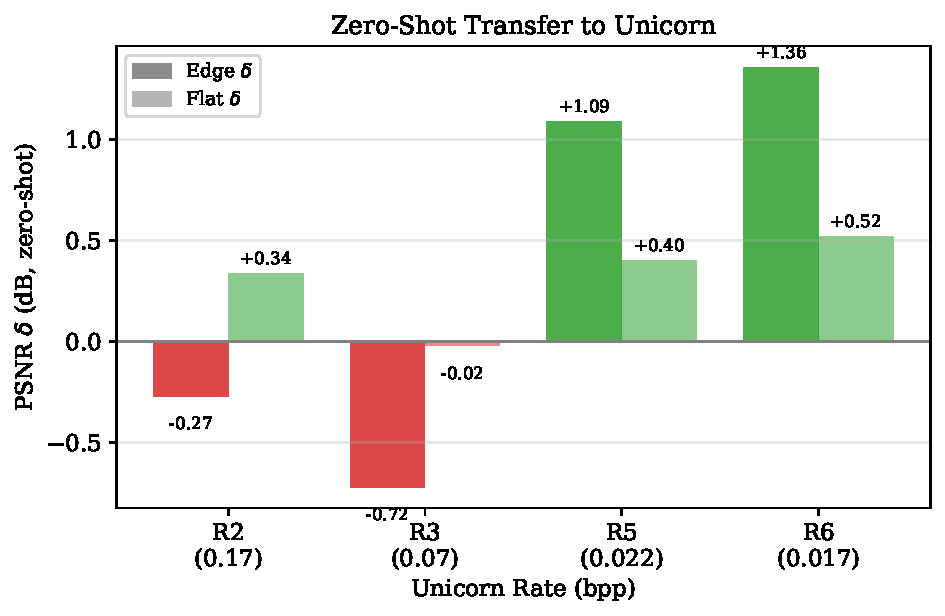
\includegraphics[width=0.72\textwidth]{unicorn_transfer.png}
  \caption{%
    Zero-shot transfer results to Unicorn.
    Green bars indicate positive PSNR improvement; red bars indicate degradation.
    Transfer succeeds at extreme rates (R5--R6, $\bpp < 0.025$)
    where oversmoothing is codec-agnostic, but degrades at moderate rates
    (R2--R3) where Unicorn's distortion pattern differs from PCGCv2's.
  }
  \label{fig:unicorn-transfer}
\end{figure}

The results show a clear bitrate threshold.
At moderate rates (R2--R4), Unicorn's distortion profile differs from PCGCv2's:
the model applies corrections calibrated for PCGCv2-style oversmoothing to a
different geometry distribution, causing slight degradation at edges.
At extreme rates (R5--R6), the oversmoothing is severe enough to be
codec-agnostic --- both PCGCv2 and Unicorn produce heavily blurred surfaces
at $\bpp < 0.025$ --- and the model's corrections transfer.

This finding has a practical implication: for scenarios where extreme geometric
fidelity is required at very low bitrates (e.g., constrained streaming),
a codec-agnostic post-processor is a viable solution.

\subsection{Zero-Shot Transfer to MVUB}
\label{ssec:mvub}

The MVUB dataset~\cite{loop2016mvub} provides upper-body captures at
resolution $G = 512$ (two sequences: \textit{david} and \textit{ricardo}),
representing an out-of-distribution test for both codec and dataset.
The model is applied without retraining.

Table~\ref{tab:mvub-results} reports the results, using BPP-corrected
rate assignment (the per-frame BPP from the actual Unicorn compressed
MVUB bitstreams).

\begin{table}[t]
  \centering
  \caption{%
    Zero-shot transfer to MVUB dataset (PCGCv2 decoded, $G=512$).
    Results averaged over 10 frames per sequence.
    BPP-corrected rate used for FiLM conditioning.
  }
  \label{tab:mvub-results}
  \begin{tabular}{llrrr}
    \toprule
    Sequence & Rate & Edge $\delta$ (dB) & Flat $\delta$ (dB) & D1 $\delta$ (dB) \\
    \midrule
    \multirow{3}{*}{david}
      & r2 & $\mathbf{+0.92}$ & $\mathbf{+0.47}$ & $-0.24$ \\
      & r4 & $-0.46$ & $-0.05$ & $-0.42$ \\
      & r6 & $-0.09$ & $-0.09$ & $-0.10$ \\
    \midrule
    \multirow{3}{*}{ricardo}
      & r2 & $\mathbf{+1.03}$ & $\mathbf{+0.43}$ & $-0.88$ \\
      & r4 & $-0.50$ & $-0.14$ & $-0.48$ \\
      & r6 & $-0.12$ & $-0.12$ & $-0.13$ \\
    \bottomrule
  \end{tabular}
\end{table}

The pattern mirrors the Unicorn transfer: positive gains at r2 (low rate),
negative at r4/r6 (moderate-high rates).
At r2, both \textit{david} ($+0.92$~dB) and \textit{ricardo} ($+1.03$~dB)
show substantial edge improvement at the rate where oversmoothing is most
severe, suggesting the correction holds across dataset and resolution.
The negative D1 $\delta$ at r2 is notable: the model improves edge quality
but slightly degrades the aggregate D1, reflecting a geometric trade-off
between edge recovery (adding sub-voxel displacements to edge points) and
flat-region precision.
This reveals a limitation of aggregate D1 as a metric for evaluating
post-processing that specifically targets non-uniform artifacts.

% ============================================================

\section{Qualitative Analysis}
\label{sec:qualitative}

Figures~\ref{fig:qualitative-soldier}--\ref{fig:qualitative-3d} present
qualitative comparisons showing the geometric improvement produced by the
post-processor.

\begin{figure}[t]
  \centering
  \includegraphics[width=0.98\textwidth]{soldier_vis.png}
  \caption{%
    \textit{Soldier} sequence, r2 (0.05~bpp).
    \textbf{Left}: original (79,529 pts).
    \textbf{Centre}: PCGCv2 decoded (76,058 pts): surface protrusions and
    structural boundaries are smoothed away.
    \textbf{Right}: proposed post-processed output (76,058 pts): fine
    geometric structure substantially recovered at helmet, shoulder hardware,
    and facial boundaries.
    Point count is preserved by construction.
  }
  \label{fig:qualitative-soldier}
\end{figure}

\begin{figure}[t]
  \centering
  \includegraphics[width=0.98\textwidth]{soldier_3d_nocurv_ep24_r2.png}
  \caption{%
    \textit{Soldier} sequence 3D view, r2 (0.05~bpp).
    \textbf{Left}: original.
    \textbf{Centre}: PCGCv2 decoded: surface geometry is noticeably blurred
    at fine structures.
    \textbf{Right}: proposed: surface sharpness partially recovered.
  }
  \label{fig:qualitative-3d}
\end{figure}

\begin{figure}[t]
  \centering
  \includegraphics[width=0.98\textwidth]{redandblack_3d_nocurv_ep24_az10_r2.png}
  \caption{%
    \textit{Redandblack} sequence, 3D view at r2 (0.05~bpp).
    \textbf{Left}: original.
    \textbf{Centre}: PCGCv2 decoded: clothing texture and body contours
    are smoothed.
    \textbf{Right}: proposed: detail partially recovered across the surface.
  }
  \label{fig:qualitative-redandblack}
\end{figure}

The qualitative improvement is concentrated at geometric boundaries and surface
structures (helmet visor, shoulder hardware, clothing texture).
The overall body shape is unchanged; the model applies corrections at
high-curvature regions rather than globally rescaling the point cloud.

% ============================================================

\section{Discussion}
\label{sec:discussion}

\paragraph{What drives the improvement.}
The $+2.06$~dB edge gain at r2 closes approximately 85\% of the
oversmoothing gap (which averages $\sim$2.4~dB across sequences at r2).
The primary driver is the dynamic Chamfer Distance loss: without it,
all displacement-based approaches fail due to zero-inflation (Table~\ref{tab:ablation-loss}).
The FiLM conditioning adds a further $+0.44$~dB at r2 over the single-rate
baseline model, a gain attributable to multi-rate regularisation.

\paragraph{The edge-flat gap after post-processing.}
After refinement at r2, the residual edge-flat gap is approximately
$62.70 - 62.11 = 0.59$~dB (from Table~\ref{tab:absolute-psnr-results}).
The residual gap is much smaller than the baseline $\sim$2.4~dB,
but not eliminated.
Two mechanisms limit further recovery:
(a) the displacement formulation cannot add points at severely undersampled
edge locations (where the codec has dropped entire voxels);
(b) the backbone's $13^3$ voxel receptive field may be insufficient for
fine structures smaller than one cell at the coarsest scale (level 3: $4\times$
downsampled, i.e., $52^3$ voxels at full resolution).

\paragraph{Processing efficiency.}
The model processes a 750K-point frame in under 300~ms on a single RTX 3090 GPU,
compared to the PCGCv2 decode step which takes 22--31 seconds.
Post-processing adds approximately 1\% to the total decode latency,
making it practical for batch applications.
Real-time use ($< 33$~ms for 30 fps) would require further optimisation,
primarily reducing the patch assembly and overlap averaging overhead.

\paragraph{Rate generalisation.}
The per-frame BPP rather than a nominal rate label is used for FiLM
conditioning, which allows the model to handle variable-bitrate output
(e.g., rate control enabled codecs) and codecs with different BPP ranges
than PCGCv2.
This is why the Unicorn and MVUB transfer experiments use BPP-corrected
rate conditioning.


% ============================================================
%  Chapter 6 -- Conclusion
% ============================================================
\chapter{Conclusion and Future Work}
\label{ch:conclusion}

% ============================================================
\section{Summary}

This thesis addressed the problem of geometric oversmoothing in learned
point cloud codecs, with a specific focus on PCGCv2 as a representative system.

We began by observing that standard aggregate quality metrics mask the
spatially non-uniform nature of codec artifacts.
To expose this, we introduced the \emph{curvature-stratified PSNR metric},
which partitions the original point cloud by local surface variation and
computes quality separately for edge (high-curvature) and flat (low-curvature)
regions.
Applied to PCGCv2 across the 8iVFB dataset, the metric revealed a consistent
and growing degradation gap of 2--4.5~dB, widening with rate --- a structural
bias of the learned codec that standard metrics do not detect.

With this diagnostic, we designed a post-processing network to correct the
identified distortions without modifying the codec.
The architecture --- a three-level sparse U-Net with a FiLM-conditioned
displacement head --- was shaped by three requirements derived from the
oversmoothing analysis:
(a) spatial awareness of surface geometry, provided by the U-Net's
multi-scale receptive field;
(b) rate adaptation, provided by the FiLM head;
(c) a training loss that avoids zero-inflation collapse, provided by the
dynamic Chamfer Distance.

The final model achieves an average edge PSNR improvement of
$\mathbf{+2.06}$~dB at the lowest evaluated rate,
$\mathbf{+0.58}$~dB at medium rate, and
$\mathbf{+0.27}$~dB at high rate,
across all four 8iVFB sequences and 400 frames.
These gains are consistent across all four sequences, including three not
seen during training.

Zero-shot transfer experiments demonstrate that the model extracts
corrections general enough to improve an unseen codec (Unicorn) at extreme
compression rates, where oversmoothing is severe enough to be codec-agnostic.

% ============================================================
\section{Contributions}

To summarise, the concrete contributions of this thesis are:

\begin{enumerate}
  \item \textbf{Curvature-stratified PSNR.}
    A diagnostic metric that separates codec evaluation by surface geometry,
    enabling targeted assessment of edge-region quality.
    The implementation is released as part of the evaluation pipeline.

  \item \textbf{Oversmoothing characterisation.}
    A systematic quantitative study showing that PCGCv2's oversmoothing gap
    grows with rate, is sequence-dependent, and is absent in G-PCC, providing
    evidence that it is a structural property of the learned encoder.

  \item \textbf{Dynamic Chamfer Distance loss.}
    A per-patch matching loss that avoids both zero-inflation collapse and
    nearest-neighbour noise, enabling successful training of a displacement
    regressor where standard losses fail.

  \item \textbf{FiLM-conditioned multi-rate post-processor.}
    A single lightweight model that serves multiple rate-distortion operating
    points, achieving better performance than per-rate models through
    beneficial multi-rate regularisation.

  \item \textbf{Evidence for cross-codec oversmoothing.}
    Zero-shot transfer results showing that at extreme compression, geometric
    oversmoothing is a codec-agnostic failure mode that a learned corrector
    can address without retraining.
\end{enumerate}

% ============================================================
\section{Limitations}

\paragraph{Single-codec training.}
The model is trained exclusively on PCGCv2-decoded clouds.
At moderate rates for other codecs (e.g., Unicorn R2--R4), transfer is
negative.
A codec-agnostic post-processor would require either multi-codec training
or a codec identification mechanism.

\paragraph{Displacement-only formulation.}
The network can only shift existing points, not add or remove them.
At very low bitrates, the decoded cloud may be missing entire surface regions
(point dropping), which displacement corrections cannot recover.

\paragraph{Dataset scope.}
All training and primary evaluation is on the 8iVFB dataset: dense,
full-body human captures at $G=1024$.
Performance on sparse outdoor LiDAR scans, mechanical parts, or lower-resolution
captures is not evaluated.

\paragraph{Computational cost.}
Post-processing adds an inference step with latency proportional to point
cloud size.
For streaming applications, this latency must be bounded; the current
implementation is not optimised for real-time use.

% ============================================================
\section{Future Work}
\label{sec:future-work}

The results open several directions for follow-up.
We group them roughly by how much new work each would require.

\subsection*{Near-Term Extensions}

\paragraph{Curriculum fine-tuning.}
The current model trains all rates jointly from the start.
A curriculum approach --- pre-training the backbone on r2 alone, then
fine-tuning the FiLM head on r4 and r6 --- may further improve mid-to-high
rate performance.
The intuition: the r2 displacement signal is the richest, so the backbone
develops strong edge-detection features from r2 data.
Fine-tuning the FiLM head separately for each rate, with the backbone frozen,
could allow the head to specialise without interference from competing
rate objectives.
Preliminary experiments with this curriculum order showed promising
convergence on validation loss at r4, but the approach was not fully evaluated
for the final paper.

\paragraph{Inference-time rate adaptation.}
The current model is conditioned on the actual BPP of each decoded cloud,
which requires metadata from the codec.
In deployment settings where the BPP is unknown, the model could estimate it
from the decoded cloud statistics (e.g., decoded point count divided by the
number of transmitted bytes, reconstructed from the occupancy pattern).
A blind BPP estimator would make the post-processor completely black-box,
requiring only the decoded point cloud.

\paragraph{Faster inference via learned patch routing.}
The sliding-window patch inference processes all patches uniformly.
At high bitrates, most patches are already close to the original surface and
require only near-identity corrections.
A lightweight ``patch quality'' predictor (e.g., based on local point density
variance) could route patches to skip inference when the estimated correction
is below a threshold, reducing inference time at high bitrates by
$50$--$70\%$ with negligible quality loss.

\subsection*{Medium-Term Research Questions}

\paragraph{Point addition via occupancy prediction.}
The displacement formulation can only shift existing points, not add new ones.
At very low bitrates (below r1), PCGCv2 drops entire surface patches, leaving
regions empty that no displacement can recover.
Extending the displacement head with an additional occupancy prediction branch
--- predicting whether new points should be inserted in empty voxels near the
current surface --- would address this limitation.
This requires a different loss: the Chamfer Distance extends naturally to
handle variable-size output sets (the CD itself does not require
fixed cardinality), but the occupancy branch introduces a combinatorial
structure that needs careful regularisation to avoid spurious insertions.

\paragraph{Attribute (colour) post-processing.}
This thesis focuses entirely on geometry.
Learned codecs also oversmooth colour attributes at high-curvature regions:
colour boundaries (e.g., the edge between a face and hair) are blurred in
the decoded cloud by the same occupancy-based encoding mechanism that blurs
geometry.
A joint geometry-and-colour post-processor using the geometric features as
context for colour refinement is a natural extension.
The shared backbone would extract edge-aware features; separate heads would
predict geometric displacements and colour residuals.
The loss would combine geometric Chamfer Distance and colour mean squared
error, with an optional edge-aware perceptual weight.

\paragraph{Temporal coherence in video sequences.}
The current post-processor is applied frame-by-frame, independently.
For volumetric video sequences at 10 fps, adjacent frames share approximately
90\% of surface geometry (a human subject moves slowly).
A temporally coherent post-processor could condition on the refined cloud
from the previous frame, propagating high-quality corrections forward in time
and reducing temporal flickering artifacts that are perceptually disturbing
in volumetric video playback.
The FiLM conditioning is a natural extension point: the temporal offset (frame
number within the GOP) could be appended to the rate scalar.

\paragraph{Multi-codec training.}
At intermediate bitrates (Unicorn R2--R4), the current model applied to
Unicorn-decoded clouds produces negative PSNR changes.
This is because Unicorn's distortion patterns differ from PCGCv2's at
non-extreme rates.
Training on a mixture of PCGCv2- and Unicorn-decoded clouds, with a codec
embedding (e.g., a one-hot or learned codec ID) as an additional conditioning
signal, would extend generalisation to intermediate rates for multiple codecs.
The FiLM head already accepts a vector conditioning input; appending the
codec embedding to the rate scalar requires minimal architectural changes.

\subsection*{Longer-Term Directions}

\paragraph{Evaluation on LiDAR sequences.}
All training and evaluation in this thesis uses the 8iVFB dataset: dense,
full-body human captures at $G = 1024$ with approximately $10^6$ points per
frame.
LiDAR point clouds (e.g., SemanticKITTI, nuScenes) have quite different
geometric properties: sparse, outdoor, with large empty regions
and a distribution of object types (cars, buildings, pedestrians).
Whether the curvature-stratified metric and the displacement post-processor
transfer to this domain is an open question.
If they do not, a LiDAR-specific training set and possibly a modified
curvature threshold (LiDAR surfaces have lower curvature density) would be
needed.

\paragraph{Perceptual quality metric integration.}
The curvature-stratified PSNR introduced in this thesis is a step toward
perceptually motivated evaluation.
A fully perceptual metric would require psychophysical experiments with
human observers, as standard in image quality assessment (SSIM, LPIPS).
For volumetric video, where the viewer can rotate the viewpoint, the
perceptual weighting of surface regions depends on the viewing direction ---
a direction-dependent metric that accounts for self-occlusion and viewing
probability would be more predictive of subjective quality.
Such a metric could then be used as the training objective for a
perception-driven post-processor.

\paragraph{Comparison with newer codecs and MPEG standardisation.}
SparsePCGC~\cite{wang2023sparsepcgc} and Unicorn~\cite{wang2025unicorn}
are the current state of the art.
Future developments in MPEG Immersive Coding (e.g., Video-based Point Cloud
Compression v2) may exhibit different oversmoothing profiles.
Applying the curvature-stratified evaluation framework systematically to all
these systems would establish whether geometric oversmoothing is a property
of the occupancy-grid paradigm in general, or specific to PCGCv2's
coarse-to-fine architecture.
This would contextualise the PCGCv2 findings within the broader trajectory
of the field and inform which architectural choices are responsible for the
edge-region quality gap.

\paragraph{Neural radiance field (NeRF) and 3D Gaussian codecs.}
Recent neural scene representations (NeRF, 3D Gaussian Splatting) are
beginning to be used for volumetric video compression.
These representations do not use explicit point clouds and are not directly
susceptible to geometric oversmoothing in the same way.
However, they exhibit their own characteristic artifacts at low bitrates
(blurriness, floaters, missing thin structures).
Developing analogous diagnostic metrics for these representations, and
learned post-processors that correct their specific failure modes, extends
the methodology developed here to a broader class of codecs.


% --- Bibliography -------------------------------------------
\cleardoublepage
\addcontentsline{toc}{chapter}{Bibliography}
\bibliography{references,thesis_refs}

% --- Appendices ---------------------------------------------
\appendix
% ============================================================
%  Appendix A -- Implementation Details and Configuration
% ============================================================
\chapter{Implementation Details}
\label{app:implementation}

This appendix provides implementation details, hyperparameter configurations,
and dataset statistics that complement the main text.

% ============================================================
\section{Codebase Structure}
\label{app:codebase}

The complete implementation is organised into four top-level packages:

\paragraph{\texttt{pcml/}.}
Core library containing:
\begin{itemize}
  \item \texttt{pcml/adapters/} --- Framework adapters (PCGCv2, G-PCC,
    pcc\_geo\_cnn\_v2). Each adapter wraps the corresponding codec via subprocess
    isolation, so each codec runs in its own conda environment with compatible
    dependencies. The \texttt{BaseAdapter} interface exposes
    \texttt{encode()}, \texttt{decode()}, and \texttt{get\_bpp()} methods.

  \item \texttt{pcml/metrics/} --- Quality metrics (\texttt{quality.py}: D1-PSNR,
    D2-PSNR, Chamfer Distance using \texttt{scipy.spatial.cKDTree};
    \texttt{curvature.py}: PCA-based curvature estimation, curvature histograms,
    stratified PSNR).

  \item \texttt{pcml/data/} --- Dataset loaders for PLY files and decoded cloud
    manifests.

  \item \texttt{pcml/visualization/} --- Rate-distortion curve plotting, spatial
    error visualisation.
\end{itemize}

\paragraph{\texttt{postprocessing/}.}
Post-processing model:
\begin{itemize}
  \item \texttt{model.py} --- \texttt{FiLMHeadSparseUNetV2} architecture
    (final model), plus earlier \texttt{FiLMSparseUNet}, \texttt{GatedSparseUNet},
    \texttt{ThresholdGatedUNet} (retained for reference).
  \item \texttt{losses.py} --- \texttt{dynamic\_chamfer\_loss} (production),
    plus earlier \texttt{L1DisplacementLoss}, \texttt{CurvatureWeightedL1},
    \texttt{MinKLoss}, \texttt{StratifiedLoss} (historical).
  \item \texttt{dataset.py} --- \texttt{MultiFrameDataset}: reads decoded cloud
    manifests, applies 48-element cube symmetry augmentation.
  \item \texttt{train.py} --- Training loop with AdamW + warm-up + cosine
    annealing. Supports multi-rate joint training with configurable weights.
  \item \texttt{inference.py} --- Sliding-window inference over full clouds.
    Handles patch overlap, aggregates displacements by averaging.
\end{itemize}

\paragraph{\texttt{scripts/}.}
Organised by function:
\begin{itemize}
  \item \texttt{scripts/setup/} --- Environment setup, dataset symlinks,
    verification.
  \item \texttt{scripts/analysis/} --- Curvature histograms, displacement
    distribution analysis, oversmoothing characterisation.
  \item \texttt{scripts/benchmark/} --- Single-frame and multi-frame codec
    benchmarking.
  \item \texttt{scripts/evaluation/} --- Full-dataset evaluation pipeline
    (\texttt{eval\_full\_dataset.py}, \texttt{compute\_all\_metrics.py},
    \texttt{run\_full\_pipeline.sh}).
  \item \texttt{scripts/plotting/} --- Figure generation for the paper and thesis.
\end{itemize}

\paragraph{\texttt{configs/}.}
YAML configuration files for all training runs. Production config:
\texttt{configs/cls\_v1\_r2.yaml} (v10-nocurv, r2+r4+r6 joint training).

% ============================================================
\section{PCGCv2 Codec Configuration}
\label{app:codec-config}

PCGCv2 is run in its default multi-scale configuration.
Table~\ref{tab:codec-config} lists the compression rates used throughout
this work, with the corresponding quantisation step sizes and measured
bitrates on the 8iVFB dataset.

\begin{table}[h]
  \centering
  \caption{%
    PCGCv2 compression rates and measured bitrates (bpp) on the 8iVFB
    dataset (average over all four sequences and 100 frames each).
  }
  \label{tab:codec-config}
  \small
  \begin{tabular}{ccc}
    \toprule
    \textbf{Rate Index} & \textbf{Quantisation Step} & \textbf{Avg BPP} \\
    \midrule
    r1 & 1 & $\approx 0.025$ \\
    r2 & 2 & $\approx 0.050$ \\
    r3 & 3 & $\approx 0.080$ \\
    r4 & 4 & $\approx 0.150$ \\
    r5 & 5 & $\approx 0.200$ \\
    r6 & 6 & $\approx 0.300$ \\
    r7 & 7 & $\approx 0.450$ \\
    \bottomrule
  \end{tabular}
\end{table}

Note that BPP values vary with sequence and frame due to differences in
point cloud size and geometric complexity.
The values above are approximate averages.
The FiLM head uses the actual per-cloud BPP as the conditioning scalar
at both training and inference time, not the nominal rate index.

% ============================================================
\section{Training Hyperparameters}
\label{app:hyperparams}

Table~\ref{tab:hyperparams} lists the complete set of hyperparameters used
to train the final v10-nocurv model.

\begin{table}[h]
  \centering
  \caption{Complete training hyperparameter configuration (v10-nocurv model).}
  \label{tab:hyperparams}
  \small
  \begin{tabular}{lll}
    \toprule
    \textbf{Category} & \textbf{Hyperparameter} & \textbf{Value} \\
    \midrule
    \multirow{4}{*}{Data} &
      Training sequences & longdress, loot, soldier \\
    & Validation sequence & redandblack \\
    & Frame stride & 12 (every 12th frame) \\
    & Training clouds per rate & $\approx 75$ (3 seq. $\times$ 25 frames) \\
    \midrule
    \multirow{4}{*}{Patches} &
      Patch size & $64^3$ voxels \\
    & Patch stride & 32 (50\% overlap) \\
    & Min points per patch & 10 \\
    & Augmentation & 48 cube symmetries \\
    \midrule
    \multirow{5}{*}{Optimiser} &
      Algorithm & AdamW \\
    & Learning rate ($\eta$) & $10^{-3}$ \\
    & Weight decay ($\lambda$) & $10^{-4}$ \\
    & Momentum ($\beta_1, \beta_2$) & 0.9, 0.999 \\
    & Gradient clipping & None \\
    \midrule
    \multirow{4}{*}{Schedule} &
      Total epochs & 30 \\
    & Warm-up epochs & 3 (linear, $10^{-5} \to 10^{-3}$) \\
    & Annealing epochs & 27 (cosine, $10^{-3} \to 10^{-6}$) \\
    & Best checkpoint & Epoch 24 (min validation loss) \\
    \midrule
    \multirow{4}{*}{Loss} &
      Loss function & Symmetric Chamfer Distance \\
    & Boundary padding & 0 (no padding) \\
    & Rate weights & $[w_{r2}, w_{r4}, w_{r6}] = [1.0, 0.3, 0.05]$ \\
    & Batch size & 8 patches \\
    \midrule
    \multirow{4}{*}{Architecture} &
      Input channels & 3 (normalised $xyz$) \\
    & Backbone channels & 32 / 64 / 128 / 64 / 32 \\
    & FiLM MLP & Linear(1,64) + ReLU + Linear(64,64) \\
    & Output & $5 \cdot \tanh(\Delta) \in [-5,5]^3$ \\
    \midrule
    \multirow{3}{*}{Hardware} &
      GPU & NVIDIA RTX 3090 (24 GB VRAM) \\
    & CPU & 12 cores / 24 threads \\
    & RAM & 64 GB \\
    \bottomrule
  \end{tabular}
\end{table}

% ============================================================
\section{8iVFB Dataset Statistics}
\label{app:dataset}

The 8iVFB~\cite{8ivfb} (8i Voxelized Full Bodies) dataset contains
four volumetric video sequences of human subjects, captured at 10 fps
and voxelized at resolution $G = 1024$:
\textit{longdress}, \textit{loot}, \textit{redandblack}, and \textit{soldier}.

Table~\ref{tab:dataset-stats} summarises the dataset statistics.

\begin{table}[h]
  \centering
  \caption{%
    8iVFB dataset statistics (averages over the first 100 frames per sequence
    at the original resolution $G = 1024$).
  }
  \label{tab:dataset-stats}
  \small
  \begin{tabular}{lcccc}
    \toprule
    \textbf{Sequence} & \textbf{Frames} &
    \textbf{Avg Points} & \textbf{Avg High-$\kappa$\%} & \textbf{Subject} \\
    \midrule
    longdress   & 300 & $\approx 857\,000$ & $\approx 33\%$ & Female, dress \\
    loot        & 300 & $\approx 805\,000$ & $\approx 33\%$ & Male, casual \\
    redandblack & 300 & $\approx 757\,000$ & $\approx 33\%$ & Male, T-shirt \\
    soldier     & 300 & $\approx 1\,089\,000$ & $\approx 33\%$ & Male, uniform \\
    \bottomrule
  \end{tabular}
\end{table}

The high-curvature fraction (top third of points by PCA curvature $\kappa$)
is approximately 33\% by construction of the stratification (tertile split).
The dataset was licensed from 8i Labs and is available at the MPEG content
repository.

For training, we use frames 1--300 of \textit{longdress}, \textit{loot},
and \textit{soldier}, with frame stride 12 (25 frames per sequence).
\textit{redandblack} is held out entirely for validation and evaluation.
For the full 400-frame evaluation, we use 100 frames from each sequence
(sampled with stride 3 from frames 1--300).

% ============================================================
\section{Evaluation Pipeline}
\label{app:eval-pipeline}

The evaluation pipeline consists of three stages:

\paragraph{Stage 1: Inference.}
\texttt{eval\_full\_dataset.py --infer\_only} runs the post-processing model
on all 400 frames $\times$ 3 rates using GPU-accelerated sliding-window
inference.
Refined clouds are saved as \texttt{.npy} files
(format: $N \times 3$ float32).
With 399 cached frames and 1 new inference, this stage takes $\approx 8$ seconds.
For a full cold run (no cache), the estimated time is $\approx 30$ minutes.

\paragraph{Stage 2: Metric computation.}
\texttt{compute\_all\_metrics.py} computes D1-PSNR, flat D1-PSNR, and edge
D1-PSNR for each frame.
Key optimisations:
\begin{itemize}
  \item \texttt{cKDTree(original)} is built once per frame and reused for all
    three metric types (forward distances), saving $\approx 3\times$ tree
    construction time.
  \item \texttt{rev\_sq\_dists} (backward distances, from original to decoded/refined)
    are computed once for D1 and reused for the stratified metric.
  \item \texttt{workers=-1} enables multi-core parallelism across frames.
\end{itemize}
Average throughput: $\approx 3$ seconds per frame.
Total for 400 frames: $\approx 20$ minutes per rate.

\paragraph{Stage 3: Aggregation.}
\texttt{run\_full\_pipeline.sh} orchestrates Stages 1--2 in parallel across
the 3 rates and merges the per-rate CSVs into a single
\texttt{nocurv\_ep24\_all.csv} with 1200 rows.

% ============================================================
\section{Software Dependencies}
\label{app:dependencies}

Table~\ref{tab:dependencies} lists the key software dependencies.

\begin{table}[h]
  \centering
  \caption{Key software dependencies for the \texttt{pcgcv2} conda environment.}
  \label{tab:dependencies}
  \small
  \begin{tabular}{lll}
    \toprule
    \textbf{Package} & \textbf{Version} & \textbf{Purpose} \\
    \midrule
    Python & 3.8 & Runtime \\
    PyTorch & 1.10.1+cu113 & Deep learning framework \\
    MinkowskiEngine & 0.5.4 & Sparse convolution \\
    CUDA & 11.3 & GPU acceleration \\
    GCC/G++ & 10.x & MinkowskiEngine compilation \\
    NumPy & 1.21 & Array operations \\
    SciPy & 1.7 & cKDTree for nearest-neighbour \\
    Open3D & 0.13 & Point cloud I/O \\
    PyYAML & 5.4 & Configuration files \\
    tqdm & 4.62 & Progress bars \\
    pandas & 1.3 & CSV result aggregation \\
    \midrule
    PCGCv2 & --- & Learned codec (git submodule) \\
    mpeg-pcc-tmc13 & --- & G-PCC codec (git submodule) \\
    pcc\_geo\_cnn\_v2 & --- & Alternative codec (git submodule) \\
    \bottomrule
  \end{tabular}
\end{table}

MinkowskiEngine must be built from source with CUDA 11.3 and GCC $\leq$ 10.
The \texttt{scripts/setup/setup\_conda\_env.sh} script automates this process,
including detecting the CUDA version and selecting the correct GCC.

% ============================================================
\section{Displacement Distribution at Each Rate}
\label{app:displacement}

Table~\ref{tab:displacement-full} provides the full displacement statistics
at all seven PCGCv2 rates for a representative 8iVFB sequence (\textit{redandblack}).
These statistics motivate the multi-rate training strategy and the static
rate weights.

\begin{table}[h]
  \centering
  \caption{%
    Displacement statistics (GT nearest-neighbour displacement magnitude
    $\|d_{gt}(\hat{p}_i)\|$ in voxels) at each PCGCv2 rate for the
    \textit{redandblack} sequence, averaged over 10 representative frames.
    ``Zero fraction'' is the fraction of points with $\|d_{gt}\| = 0$.
  }
  \label{tab:displacement-full}
  \small
  \begin{tabular}{cccc}
    \toprule
    \textbf{Rate} & \textbf{Mean $\|d_{gt}\|$} &
    \textbf{90th pct.} & \textbf{Zero fraction} \\
    \midrule
    r1 & 0.32 & 1.41 & 40\% \\
    r2 & 0.15 & 1.06 & 60\% \\
    r3 & 0.09 & 0.82 & 71\% \\
    r4 & 0.06 & 0.62 & 79\% \\
    r5 & 0.05 & 0.50 & 83\% \\
    r6 & 0.04 & 0.38 & 87\% \\
    r7 & 0.02 & 0.21 & 89\% \\
    \bottomrule
  \end{tabular}
\end{table}

The table shows clearly why training at r7 is unproductive: 89\% zero targets
with mean displacement 0.02 voxels (below quantization resolution) leave
essentially no learnable signal.
The three training rates r2, r4, r6 span the range where correction is both
needed (non-trivial zero fraction) and feasible (sub-voxel mean displacement
within the model's $\pm5$-voxel output bound).


\end{document}
